\bookpart{数学与机器学习}{Mathematics and Machine Learning}
\label{part:mathematics-and-machine-learning}

\BookPartGuide{%
前五个部分建立了函数、空间、随机变量、状态与策略的数学语言。
本部分用这些语言界定学习问题中的训练样本、评价样本、候选模型类、目标与约束、学习规则。
环境与观测机制规定记录的分布，采样机制规定整批样本的联合规律；
学习规则构造训练目标并选择训练模型，预测与评价再分别检验它的输出和表现。
行动影响后继状态时，还需用转移核、策略核和轨迹律描述反馈。

本部分只有第17章“数学基础与后续研究”。该章从温度预测与散热任务出发，
先定义共同组成，再比较固定条件、条件变化和行动反馈下的学习问题。
同一组数学对象上的问题按表示与逼近、优化与收敛、观测与统计、扰动与响应、
跨分布学习、约束与动态展开，分别说明所求量、误差和成立条件。
章节保留两层对应：从机器学习任务查到数学问题，再从数学问题查到前文知识与适用工具。
训练模型、最优解、更新序列和执行轨迹使用各自的比较标准；有限样本的估计与总体规律的识别也分别处理。
具体模型中的算法、证明与专门结论由后续各卷继续展开。}

\chapter{数学基础与后续研究}
\label{chap:mathematics-and-future-research}

用设备的温度记录训练预测器，平均训练损失已经下降，仍有哪些问题没有回答？
传感器可能漏掉决定后继温度的工况，候选模型类可能只能表达过于简单的关系，
优化程序也可能尚未求得训练目标的最优解。即使训练问题求解准确，
有限训练样本得到的模型能否用于新设备，还需要统计证据；
将预测用于散热决策以后，测量误差会不会经反馈积累，又成为轨迹上的问题。
这些困难发生在同一个学习过程中，所比较的对象和要求却各不相同。

前面各章已经建立函数、空间、概率、优化和演化的数学语言。
本章用这些语言把学习问题拆成可以判断的命题：给定什么对象，允许什么变化，
用什么量衡量结果，以及希望证明什么。
机器学习问题到数学问题的对应在第~\ref{sec:future-learning-question-inventory}节建立，
数学问题到知识与工具的对应在第~\ref{sec:future-mathematical-question-map}、\ref{sec:future-mathematical-tool-roles}节展开。
两步之间保留同一组对象与问题编号，便于查找，也便于检查某个工具的条件是否满足。
本章提供分析入口；各类模型的具体算法和专门结论由后续各卷展开。

\section{学习问题的共同构成}
\label{sec:future-unified-learning-framework}
\label{sec:future-learning-data-and-use}

训练需要一批可用记录、一组允许选择的模型，以及比较和选择模型的规则。
评价还要另行说明用哪些记录、代表哪个总体、采用什么指标。
因此，学习问题的共同组成包括训练样本与评价样本的生成规律、候选模型类、目标与约束，
以及把训练样本转成训练模型的学习规则。
下面沿用温度预测的例子逐项明确这些对象，再补充行动参与记录生成时的反馈关系。

\subsection{训练样本与评价样本的生成规律}
\label{sec:future-learning-data-objects}

温度记录来自设备运行中的具体情形。令$s\in S$包含当前真实温度、工况和指定时距后的真实温度，
其中某些量可能无法测量。要描述反复运行会遇到哪些情形，选定可测空间$(S,\Sigma_S)$
及其上的概率测度$\mu$，并将
\begin{equation}
  \mathcal E=(S,\Sigma_S,\mu)
  \label{eq:future-static-environment}
\end{equation}
称为静态环境模型。$S$是情形的集合，$\Sigma_S$规定哪些情形事件可以讨论概率，
$\mu$规定这些事件的发生概率。$\mathcal E$描述整类运行情形及其概率规律，$s$只表示其中一次情形。
行动影响后继状态时，还要加入转移规律；其定义见本节末的交互学习过程。

真实情形与实际记录未必相同：传感器可能带噪声，部分字段可能缺失，标签也可能延迟取得。为描述这些差别，需要规定观测机制。
令$(\mathsf Z,\Sigma_Z)$为记录空间，观测机制为从$S$到$\mathsf Z$的
概率核（probability kernel）$K$。它是二元函数
$K:S\times\Sigma_Z\to[0,1]$：固定$s$后，$K(s,\cdot)$是记录空间上的概率测度；
固定可测记录事件$B$后，$s\mapsto K(s,B)$是可测函数。
也就是说，$K(s,B)$回答的是：真实情形固定为$s$后，测量与标注会以多大概率产生属于$B$的记录。
它可以同时包含传感器噪声、特征提取、缺失和标注过程。
将记录空间与核合记为$\mathcal O=(\mathsf Z,\Sigma_Z,K)$。

令$V$为取值于$S$的随机变量，$Z$为取值于$\mathsf Z$的记录随机变量。
指定$V\sim\mu$以及给定$V=s$时的记录律$K(s,\cdot)$，便得到
\begin{equation}
  P(B)=\mathbb P\{Z\in B\}
      =\int_S K(s,B)\,\mu(\mathrm ds),
  \qquad B\in\Sigma_Z.
  \label{eq:future-observation-law}
\end{equation}
记$P=\mu K$。式中$P$是记录的分布，$Z$是随机变量，$z$是它的一次实现。
随机变量本身仍是从底层概率空间到取值空间的可测映射；
$V\sim\mu$与$Z\mid V=s\sim K(s,\cdot)$规定其联合分布，描述两阶段抽样。
从$(\mu,K)$计算$P$是确定的分布运算，从$P$取得一次$z$则是随机试验。

确定性观测是这个定义的特例。若记录由可测函数$g:S\to\mathsf Z$给出，
就有$Z=g(V)$、$K(s,\cdot)=\delta_{g(s)}$，其中$\delta_{g(s)}$是在$g(s)$处的点质量；
此时$P=g_{\#}\mu$是推前测度。
例如真实情形$s=(v,y)$包含当前与后继温度，记录为$(v+\xi,y)$，
其中$\xi$是独立测量噪声。给定$s$后仍需抽取$\xi$，所以通常不存在仅以$s$为自变量的确定性记录函数；
把噪声也列为自变量以后，$(s,\xi)\mapsto(v+\xi,y)$才是确定性映射。
因此，观测核描述给定真实情形后的随机测量；把测量噪声也作为自变量时，才得到描述同一测量过程的确定性函数。

一条记录的分布还没有规定多条记录的关系。
采样机制$\Gamma_n$指定预算为$n$时整批记录的联合律，记为
$Q_n=\Gamma_n(\mathcal E,\mathcal O)$，它是$\mathsf Z^n$上的概率测度。
机制本身包含独立抽取、连续采集或按历史选择等规则；单次边缘分布$P$不能决定这些规则。
有限训练样本写为有序记录组$D=(Z_1,\ldots,Z_n)$，其中每条记录可以包含训练特征和标签；有序写法保留采集顺序与重复记录。
独立同分布（independent and identically distributed, i.i.d.）采样的特例为
\begin{equation}
  D\sim Q_n=P^{\otimes n},\qquad P^{\otimes n}\text{也简记为 }P^n.
  \label{eq:future-sampling-law}
\end{equation}
上述分布用于定义问题，可以是学习者未知的真实规律；写出它们不表示算法能够读取它们。
抽样前$D$是随机对象；抽样后固定的记录组是它的一次实现，后文为简洁仍记为$D$。
评价样本也需要自己的环境、观测和采样机制。分别用下标$\mathrm{tr}$与$\mathrm{ev}$
表示训练样本和评价样本的生成规律；两者相同或独立都是附加假设。
用于候选选择的评价样本称为验证样本，用于选择完成后独立检验的评价样本称为测试样本。
修改已经取得的训练样本$D$、改变训练分布$P_{\mathrm{tr}}$、改变训练采样机制$\Gamma_{\mathrm{tr},n}$，
影响的是不同对象。后文比较结果时会分别写明这些变化。

\subsection{候选模型类的界定}
\label{sec:future-candidate-model-class}

同一组温度特征可以交给仿射函数，也可以交给非线性函数；两种方法允许选择的预测规则不同。
令$\mathsf H$为当前任务中可讨论的模型空间。在监督预测中，其元素是从预测输入空间$\mathsf X$
到预测输出空间$\mathsf Y$的可测函数。学习规则允许选择的子集$\mathcal H\subseteq\mathsf H$
称为候选模型类，单个$h\in\mathcal H$称为候选模型。候选模型类确定表达范围，尚未指定训练最终选出哪一个模型。

若用参数描述候选，定义映射$\Phi:\Theta\to\mathcal H$，令
$h_{\bm\theta}=\Phi(\bm\theta)$，其中$\Theta\subseteq\mathbb R^p$、$p$为参数维度。
下文取$\mathcal H=\Phi(\Theta)$；参数化不能覆盖事先给出的候选集合时，应以其实际的像为训练范围。
不同参数可以描述同一函数，因此增加参数数量不必然扩大候选模型类。
概率建模或策略学习可以分别以概率模型或策略核为候选，但同样需要明确候选的取值空间与允许范围。

\subsection{训练目标、评价目标与约束的界定}
\label{sec:future-learning-goal-objects}

候选模型类告诉我们能够选什么，却没有给出选择依据。
为比较预测错误，需要定义损失：用$\ell:\mathsf H\times\mathsf Z\to\mathbb R$给每个候选$h$及记录$z$计分，
并假定所讨论的损失可测、相关期望有限。
例如$z=(x,y)$时，可取$\ell(h,z)=(h(x)-y)^2$。
在无监督任务中$z$可以只有$x$，但仍需明确重构、分组或密度拟合的计分规则。

评价分布规定这些错误按什么频率计入目标。
静态任务中给定评价记录律$P$，总体风险为
\begin{equation}
  R_P(h)=\int_{\mathsf Z}\ell(h,z)\,P(\mathrm dz).
  \label{eq:future-unified-population-risk}
\end{equation}
$\ell$是以候选和记录为自变量的函数，$R_P$是以候选模型为自变量、输出一个实数的泛函。
训练分布$P_{\mathrm{tr}}$、验证分布$P_{\mathrm{va}}$与测试分布
$P_{\mathrm{te}}$需要分别指定；只有明确作出同分布假设时才统一记为$P$。
训练样本参与模型拟合，验证样本用于选择候选模型类、目标权重或学习规则，测试样本用于选择完成后的评价。
这些职责不自动保证各组样本独立或同分布；测试分布代表哪个总体，是风险定义的一部分。

约束$\mathcal C\subseteq\mathsf H$是满足任务要求的决策集合。
它可以由一组条件定义，例如$\mathcal C=\{h:c_j(h)\leq0,\ j=1,\ldots,m\}$，
其中$c_j$是约束泛函，$m$是约束数目。
对温度预测器，条件可以限制指定工况下的大误差概率；对加热策略，则可以限制越过安全温度的概率。
这些总体条件依赖未知分布时，训练中采用的经验约束只是一种估计，必须另行检查总体可行性。
最小化平均损失与满足约束是两项要求；把违规代价加入损失也会形成新的目标，
不能未经分析就认定它等价于硬约束。
候选约束与候选模型类共同确定可行范围
$\mathcal H_{\mathcal C}=\mathcal H\cap\mathcal C$。
由模型结构造成的范围限制与任务要求的行为约束有不同来源，应分别说明。
本章将损失与候选约束合记为目标设定$\mathcal T=(\ell,\mathcal C)$，评价分布由评价样本生成规律给定。
限制隐私泄露或计算资源时，约束对象还包括学习规则或计算过程；
这类约束不能只写成一个固定预测函数的性质。

\subsection{学习规则与训练、预测、评价过程}
\label{sec:future-learning-common-objects}
\label{sec:future-sampling-and-empirical-objective}
\label{sec:future-population-empirical-computation}

训练样本、候选模型类和任务目标确定以后，还需规定怎样构造训练目标、怎样更新变量，以及何时停止。
本章把包含候选范围、目标构造、初始化、更新、停止与模型读出的完整选择过程称为学习规则。
一次变量更新只是学习规则的一部分。

训练目标构造规则将有限训练样本$D$转成可计算的目标泛函$F_D$。
用$B$表示目标构造规则。固定损失、约束和候选模型类后，它是从$\mathsf Z^n$
到“实值泛函与候选子集”的映射，写为
$B(D)=(F_D,\widehat{\mathcal H}_{\mathcal C,D})$，其中
$F_D:\mathcal H\to\mathbb R$，$\widehat{\mathcal H}_{\mathcal C,D}\subseteq\mathcal H$
是实际训练中使用的可行集，亦记为$\mathcal K_D$。已知约束直接使用$\mathcal H_{\mathcal C}$；未知总体约束则需估计。
在同分布且可直接观察损失的基准设定中，\term{经验风险}（empirical risk）是样本平均损失。
以它为$F_D$，并在给定可行类中选择极小值，得到\term{经验风险最小化}
（empirical risk minimization, ERM）：
\begin{equation}
  \widehat R_D(h)=\frac1n\sum_{i=1}^n\ell(h,Z_i),\qquad
  \widehat h_D\in\argmin_{h\in\mathcal H_{\mathcal C}}\widehat R_D(h).
  \label{eq:future-unified-empirical-problem}
\end{equation}
这里假定极小值能达到。加入正则项时可取
$F_D(h)=\widehat R_D(h)+\lambda\Omega(h)$，其中$\Omega$为惩罚泛函、$\lambda\geq0$为权重。
跨分布学习可能需要加权，缺失标签可能需要代理损失；这些构造都须解释怎样联系评价目标。
训练中引入的计算便利条件也应与原任务要求区分。

参数更新规则利用$F_D$生成训练状态；停止与读出规则再把有限步状态转成训练模型。
将初始化、小批量索引等算法随机性汇集为随机变量$U$，取值空间为$\mathsf U$、分布为$\nu$。
固定学习规则后，第$k$步的训练模型由学习映射给出：
\begin{equation}
  A^{(k)}:\mathsf Z^n\times\mathsf U\to\mathcal H,
  \qquad h_D^{(k)}=A^{(k)}(D,U).
  \label{eq:future-learning-algorithm-output}
\end{equation}
对不同样本数，实际使用映射族$\{A_n^{(k)}\}$；上式省略下标$n$。
比较删除或增加记录前后的输出时，分别调用对应样本数的成员。
这里$A^{(k)}$是目标构造与求解的复合映射；$F_D$是其中的中间对象。
若算法允许中间迭代违反约束，$A^{(k)}$的值仍属于$\mathcal H$，却未必属于可行类；
后面的风险最优化保证在使用可行性时会显式要求输出可行。
为讨论输出概率，在候选空间上给定适当的可测结构，并要求$A^{(k)}$可测。
基准设定令$U$独立于$D$。有限预算固定后将训练模型简记为$h_D$。
参数、动量等构成训练状态$v_D^{(k)}$，优化器可以写成
$v_D^{(k+1)}=T_{D,k}(v_D^{(k)},U_k)$，再从状态读出$\bm\theta^{(k)}$和$h_D^{(k)}$。
计算步$k$、样本数$n$和环境时间$t$是三个不同的索引。

将优化程序（含初始化、更新、停止与输出规则）记为$\mathscr A$，
学习规则记为结构$\mathcal L=(\mathcal H,\Phi,B,\mathscr A)$。
对阶段$r\in\{\mathrm{tr},\mathrm{va},\mathrm{te}\}$，用
$\mathcal G_r=(\mathcal E_r,\mathcal O_r,\Gamma_r)$记录该阶段的环境、观测与采样规则族；
样本生成设定为$\mathcal D=(\mathcal G_{\mathrm{tr}},\mathcal G_{\mathrm{va}},\mathcal G_{\mathrm{te}})$。
因此$\mathcal D$记录三类样本的生成规律，与一批实现样本$D$不同。完整学习设定记为
\begin{equation}
  \mathcal M=(\mathcal D,\mathcal T,\mathcal L).
  \label{eq:future-unified-learning-problem}
\end{equation}
写$R_{\mathcal M}$时，表示使用该设定中的评价分布和损失；静态情形仍简记为$R_P$。
总体解集合$\mathcal H^\star_{\mathcal M}=\argmin_{h\in\mathcal H_{\mathcal C}}R_{\mathcal M}(h)$、
理想训练解$\widehat h_D$与有限步训练模型$h_D^{(k)}$因此各有不同含义。
样本随机性改变训练问题，算法随机性改变同一训练问题中的求解过程。

\paragraph{固定训练模型的预测与评价}
\label{sec:future-static-learning-process}

训练将有限训练样本映成训练模型$D\mapsto h_D$；预测则固定$h_D$，将预测输入映成预测输出$x\mapsto h_D(x)$。
监督任务中的记录$z=(x,y)$用于计算损失，部署预测时通常只给模型$x$。
标签$y$若需延迟获取，评价也须遵守这一信息条件。
图~\ref{fig:future-unified-learning-framework}中的箭头分别表示确定的分布构造、随机采样、
目标构造、求解与评价，不能都理解成同一种函数运算。

\begin{figure*}[htbp]
  \centering
  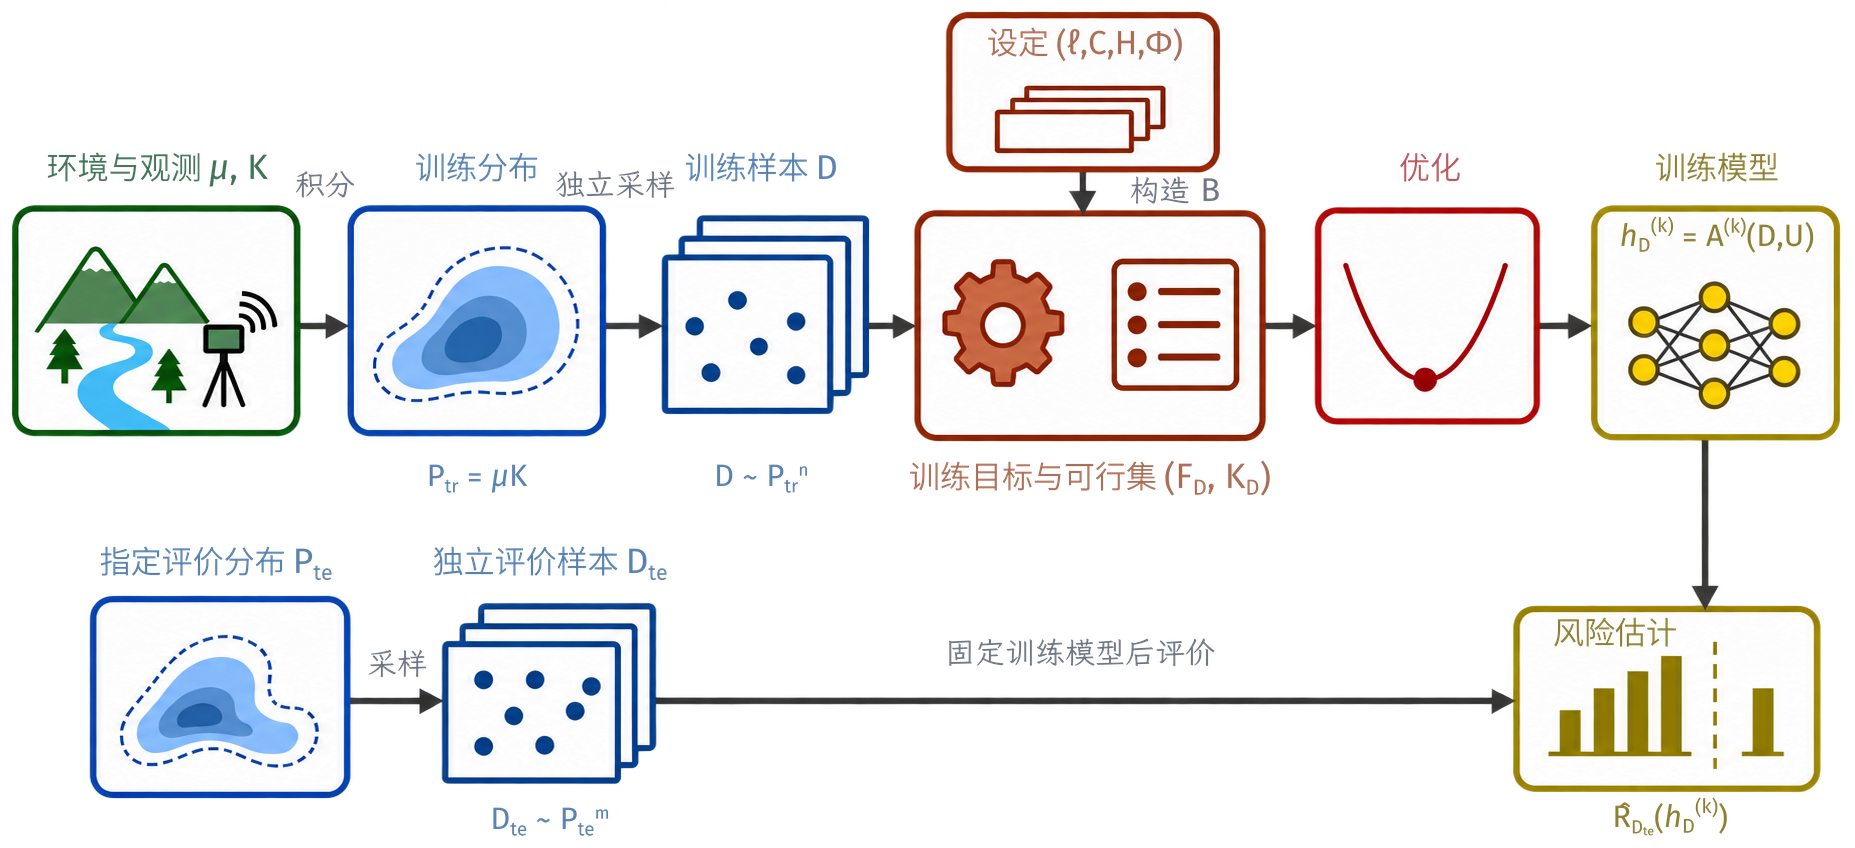
\includegraphics[width=\linewidth]{figures/01-mathematical-preliminaries/06-mathematics-and-machine-learning/generated/static-learning-framework/figure.png}
  \caption{静态学习中的样本生成、目标与学习规则。图中取独立采样$Q_n=P_{\mathrm{tr}}^n$；
  $P_{\mathrm{tr}}=\mu K$是分布运算，$D\sim Q_n$是采样。
  目标构造$B$与优化规则共同组成学习映射$A$。
  固定训练模型后，独立测试记录用于估计指定测试分布下的评价风险。}
  \label{fig:future-unified-learning-framework}
\end{figure*}

固定$h_D$以后，若另取独立测试集$D_{\mathrm{te}}\sim P_{\mathrm{te}}^m$，
样本平均$\widehat R_{D_{\mathrm{te}}}(h_D)$估计的是$R_{P_{\mathrm{te}}}(h_D)$。
这里的测试分布是当前任务规定的评价总体。
若测试集实际来自另一分布，还须说明两者的联系，不能仅凭样本平均代表指定的测试风险。
同一分布下两批有限样本不同，可以只是抽样波动；
训练分布与测试分布不同，则需要增加分布之间的假设与分析。

\paragraph{行动反馈下的轨迹生成}
\label{sec:future-interactive-learning-process}

加热行动会改变后继温度，这时单次情形分布不足以描述环境。
在有限时域、受控Markov模型的简化设定中，取状态空间$(S,\Sigma_S)$、
行动空间$(\mathsf A,\Sigma_A)$、初始状态分布$\mu_0$，以及转移概率核
$T:S\times\mathsf A\times\Sigma_S\to[0,1]$。
对每个$(s,a)$，$T(s,a,\cdot)$是下一状态的概率测度；对每个状态事件，核关于$(s,a)$可测。
动态环境模型是结构
\[
  \mathcal E=(S,\Sigma_S,\mathsf A,\Sigma_A,\mu_0,T).
\]
它增加了行动影响状态的规律。此处同一个符号$\mathcal E$按明确声明的静态或动态设定使用，
不会把静态三元组直接当作转移函数。

观测核$K_o:S\times\Sigma_O\to[0,1]$在状态给定后生成观测$o_t$，
$(\mathsf O,\Sigma_O)$为观测空间。可见反馈也可以包含在$o_t$中。
令$I_t=(o_0,a_0,\ldots,a_{t-1},o_t)$为可得历史；
策略$\pi_t$是从历史空间到行动空间的概率核，给出$\pi_t(\mathrm da\mid I_t)$。
确定性策略是点质量核，完全可观测情形才可直接以当前状态为决策依据。

固定环境、观测机制和策略。长度为$H$的理论轨迹记为
\[
  \tau=(s_0,o_0,a_0,\ldots,a_{H-1},s_H,o_H).
\]
它的联合律为
\begin{equation}
  \begin{aligned}
    P_{\mathcal E}^{\pi}(\mathrm d\tau)
    ={}&\mu_0(\mathrm ds_0)K_o(s_0,\mathrm do_0)\\
      &\cdot\prod_{t=0}^{H-1}
      \pi_t(\mathrm da_t\mid I_t)
      T(s_t,a_t,\mathrm ds_{t+1})K_o(s_{t+1},\mathrm do_{t+1}).
  \end{aligned}
  \label{eq:future-interactive-trajectory-law}
\end{equation}
$P_{\mathcal E}^{\pi}$的简记还隐含固定的$K_o$与时域$H$；比较观测机制时必须把其依赖恢复。
每个因子对应一次条件采样，乘积规定整条轨迹的联合分布。
理论轨迹可包含隐状态，实际记录只能包含采集到的字段；实际记录律是上述轨迹律经记录映射的推前。
累计成本写为可积轨迹损失$\ell(\pi,\tau)$，则
$R_{\mathcal M}(\pi)=\mathbb E_{P_{\mathcal E}^{\pi}}[\ell(\pi,\tau)]$。
若损失依赖未观测状态，还需另行论证能否从记录识别它。

行为策略$\beta$采集训练轨迹样本，目标策略$\pi$是所要学习或评价的策略。
为与静态学习的记录分布对应，以$\mathsf T_H$表示长度为$H$的理论轨迹空间，
$\mathsf Z_{\mathrm{rec}}$为可见记录空间，固定可测记录映射
$b:\mathsf T_H\to\mathsf Z_{\mathrm{rec}}$。轨迹律与记录分布分别是
\[
  P_{\mathcal E}^{\sigma},\qquad
  P_{\mathrm{rec}}^{\sigma}=b_{\#}P_{\mathcal E}^{\sigma},
  \qquad \sigma\in\{\beta,\pi\}.
\]
记录映射可以去掉隐状态等不可采集字段；它将轨迹律推前为实际记录分布。
在独立重复完整运行的基准设定中，训练样本满足
$D\sim(P_{\mathrm{rec}}^{\beta})^n$。
固定训练得到的策略$\pi$后，给定训练样本及算法随机性，
用新的环境随机性独立重复运行取得$D_{\mathrm{te}}\sim(P_{\mathrm{rec}}^{\pi})^m$。
每个样本是一条完整轨迹的可见记录，同一条轨迹内的时刻并不因此独立。

即使两者使用同一环境，$P_{\mathcal E}^{\beta}$与$P_{\mathcal E}^{\pi}$也可能不同。
离线学习须说明旧策略的记录怎样支持新策略的评价；在线学习还会让后续采样依赖已有学习结果。
图~\ref{fig:future-interactive-learning-framework}中，两个策略连接同一个环境节点。
采集阶段由$\beta$选择行动，执行阶段改用固定的$\pi$；每个阶段中，
行动都反馈到环境，新的观测进入历史，再决定后续行动。
两种策略与环境分别诱导轨迹律，经$b$得到可见记录分布，再采样得到有限轨迹样本。
这与图~\ref{fig:future-unified-learning-framework}中由记录分布采样得到训练或测试样本的读法相同，
但交互任务的分布还依赖参与训练记录与评价记录生成的策略。

若存在可积的记录损失$\ell_{\mathrm{rec}}$，使
$\ell_{\mathrm{rec}}(\pi,b(\tau))=\ell(\pi,\tau)$，
则对测试记录$D_{\mathrm{te}}=(Z_1,\ldots,Z_m)$，总体风险与样本估计可以写为
\[
  \begin{aligned}
    R_{\mathcal M}(\pi)
      &=\mathbb E_{P_{\mathrm{rec}}^{\pi}}[\ell_{\mathrm{rec}}(\pi,Z)],\\
    \widehat R_{D_{\mathrm{te}}}(\pi)
      &=\frac1m\sum_{j=1}^m\ell_{\mathrm{rec}}(\pi,Z_j).
  \end{aligned}
\]
样本估计与总体轨迹风险的关系需要统计分析，不能从一次测试直接读取总体期望。

\begin{figure*}[htbp]
  \centering
  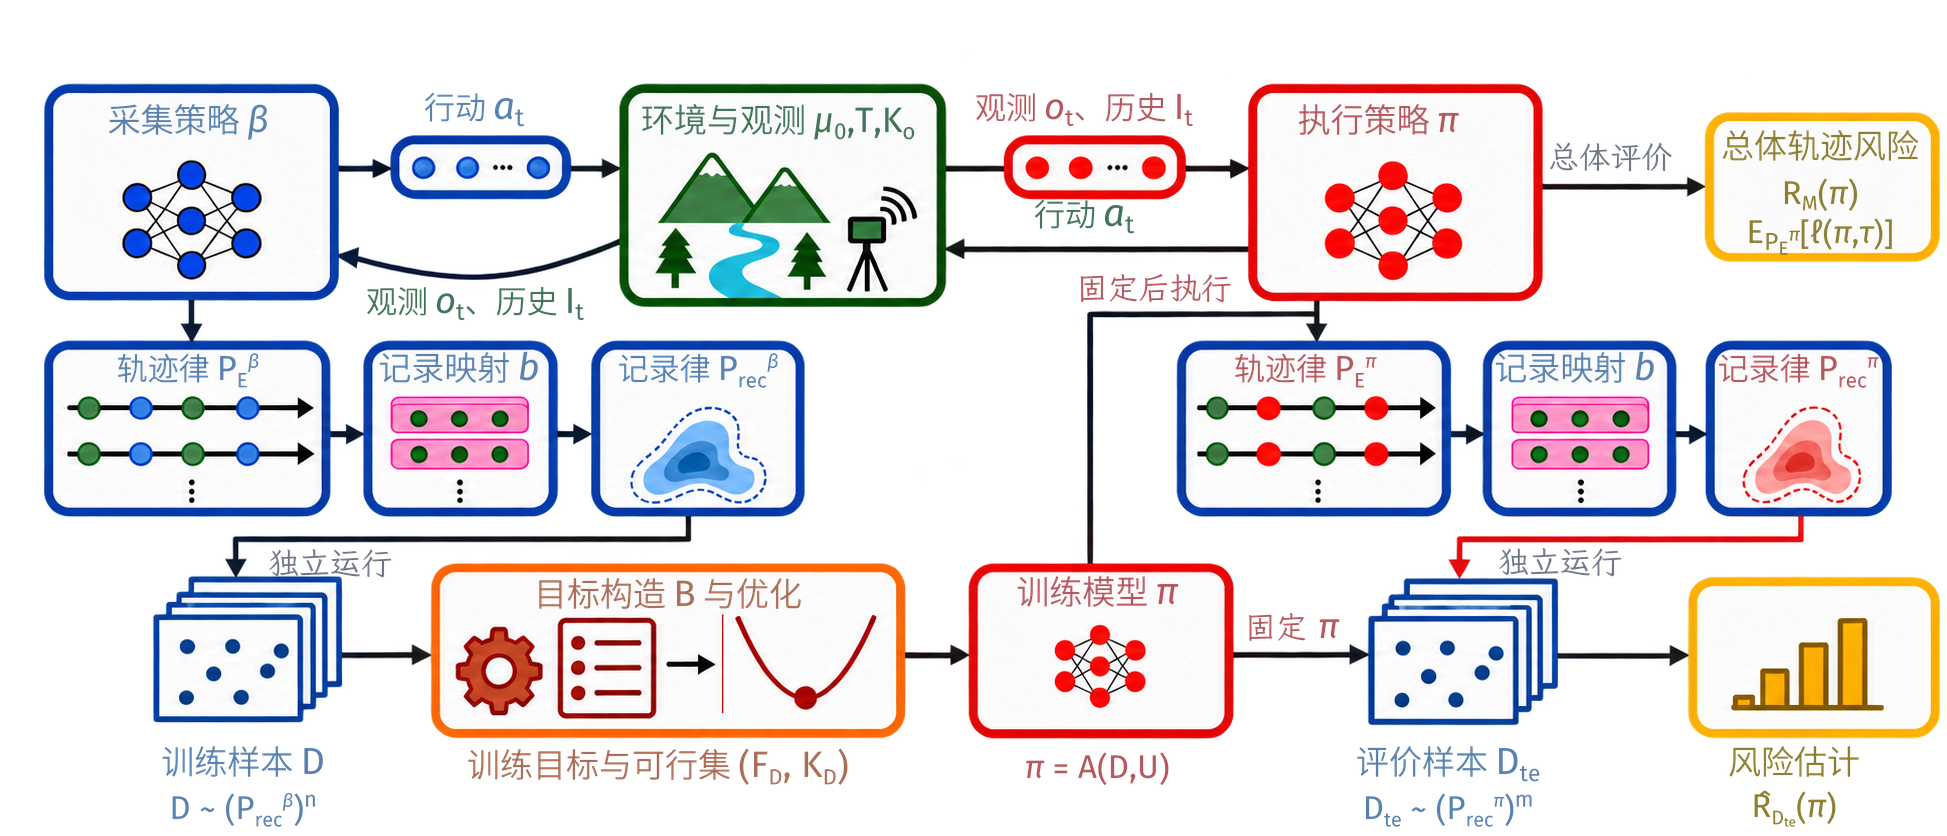
\includegraphics[width=\linewidth]{figures/01-mathematical-preliminaries/06-mathematics-and-machine-learning/generated/interactive-learning-framework/figure.png}
  \caption{同一环境中的交互学习及其分布、记录与评价。
  采集策略$\beta$与执行策略$\pi$分阶段接入同一个环境，行动返回环境，观测$o_t$进入历史$I_t$。
  记录分布由轨迹律经记录映射$b$推前得到。图示取完整运行之间独立，
  固定训练得到的策略后重新采集测试轨迹，且轨迹损失可由可见记录计算。
  总体轨迹风险由期望定义，独立测试记录给出相应的样本风险估计。}
  \label{fig:future-interactive-learning-framework}
\end{figure*}

\begin{table*}[htbp]
  \centering
  \begin{tabularx}{\linewidth}{lXXX}
    \toprule
    学习形式 & 训练样本与评价样本 & 目标 & 候选模型或策略\\
    \midrule
    有监督学习 & 预测输入与标签的联合记录$(x,y)$ & 预测损失与行为约束 & 预测函数$h:\mathsf X\to\mathsf Y$\\
    无监督学习 & 无标签的预测输入记录$x$ & 重构、分组或密度目标 & 表示、簇中心或概率模型$q_h$\\
    强化学习 & 策略参与生成的轨迹记录 & 累计成本、负回报与轨迹约束 & 从可得历史选择行动的策略$\pi$\\
    \bottomrule
  \end{tabularx}
  \caption{三类学习任务使用相同的组成对象，但记录、候选和目标的具体类型不同。
  概率模型$q_h$给出的模型分布须与真实观测分布$P$区分。}
  \label{tab:future-learning-paradigm-interfaces}
\end{table*}

\FloatBarrier
\section{不同学习设定下的问题表述}
\label{sec:future-learning-question-inventory}

前一节定义了学习设定中的组成。本节从具体任务出发，明确哪一个数学对象接受分析。
一项完整表述要给出对象的类型、定义域和值域，说明哪些量固定、哪些量改变，
再指定误差、距离、事件或极限。例如，固定样本$D$后的预测函数
$h_D:\mathsf X\to\mathsf Y$，与把样本映成预测函数的
$A^{(k)}:\mathsf Z^n\times\mathsf U\to\mathcal H$，是两个不同的映射。
前者接受预测输入$x$的扰动，后者接受训练样本$D$的扰动，不能只用“模型鲁棒性”代替这一差别。

以下沿用温度预测、越限预警与自动散热的教学场景。
对可测空间$\mathsf B$，以$\mathcal P(\mathsf B)$表示其上的概率测度集合，
以$2^{\mathsf B}$表示其所有子集组成的集合。
涉及随机映射与上确界事件时要求可测，涉及积分时要求可积；条件分布在其存在的空间中讨论。
函数距离、集合距离与概率测度距离分别指定，不能把这些对象都当成可直接相减的实数。
本节在实际任务中写出对象与分析量；下一节合并相同数学结构的问题，给出正式问题和数学工具的入口。

以下把固定条件下的学习、条件改变后的学习与行动反馈下的策略学习分开。
固定条件是指训练样本生成规律、评价样本生成规律、候选模型类、训练目标、约束和学习规则已经指定，
并不要求训练分布与评价分布相同。对其中某项进行对照变更时，需明确变更对象与共同评价标准；
行动改变后继观测时，则必须把策略反馈纳入样本的联合规律。

\subsection{固定训练与评价条件下的学习问题}
\label{sec:future-fixed-learning-conditions}

\paragraph{统计目标的识别与候选模型的表达}
\label{sec:future-ml-information-expression}

设设备需要提前一段时间预测温度，预测输入$x$包含温度读数、负载或控制记录，
标签$y$是指定时距后的温度。回归预测器$h:\mathsf X\to\mathbb R$输出温度值，
平方损失为$\ell(h,(x,y))=(h(x)-y)^2$。
若改为越限预警，则由阈值$c$构造二元标签$\mathbb I\{y>c\}$，
候选的输出空间和漏报、误报的损失也随之改变。同一批原始记录可以服务于不同的数学任务。

如果加热动作影响后继温度，却没有进入记录，不同的作用机制可能产生相同的温度记录分布。
为表述这种信息歧义，固定状态空间、记录空间和观测核$K$，令$\mathfrak E$为允许的静态环境模型集合，
$\mathsf J$为目标量的取值空间。先考虑独立重复采样$Q_n^{\mathcal E}=(\mu K)^{\otimes n}$，
此时单条记录的分布决定全部样本律。需要分析的是两个映射
\begin{equation}
  \begin{aligned}
    \Xi&:\mathfrak E\to\mathcal P(\mathsf Z),
      &\Xi(\mathcal E)&=\mu K,\\
    J&:\mathfrak E\to\mathsf J,
      &\mathcal E&\mapsto J(\mathcal E).
  \end{aligned}
  \label{eq:future-task-observation-target-maps}
\end{equation}
$\Xi$输出可观测记录的分布，$J$输出希望确定的温度规律或参数。
\textbf{可识别性分析}检查：对任意$\mathcal E,\mathcal E'\in\mathfrak E$，
$\Xi(\mathcal E)=\Xi(\mathcal E')$是否蕴含$J(\mathcal E)=J(\mathcal E')$。
这里比较的是环境在两个映射下的像；如果观测相同而目标不同，增加同类记录不能自行消除歧义。
若实际采用相关或自适应采样，应将$\Xi$改为完整可观测联合律或观测实验族$(Q_n^{\mathcal E})_n$。
单条记录的边缘律相同，并不意味着多条记录之间的关系也相同，后者可能提供额外信息。
若所求量是干预效果，应先将因果结构加入环境模型，再定义$J$与相应的观测映射；
仅给出静态观测分布还没有定义一个干预模型。

信息充分以后，还要检查方法允许的候选能否表示所需规律。
例如，仿射函数不能在非退化区间上处处表示二次温度规律。
固定参考函数$g\in\mathsf H$、函数距离$d_{\mathsf H}$和表示映射
$\Phi:\Theta\to\mathcal H\subseteq\mathsf H$，令
$\Theta_{\mathcal C}=\{\bm\theta\in\Theta:\Phi(\bm\theta)\in\mathcal C\}$。
\textbf{表示与逼近分析}的对象及比较量为
\[
  \mathcal H_{\mathcal C}=\Phi(\Theta_{\mathcal C}),\qquad
  e_{\mathrm{app}}(g)=
  \inf_{\bm\theta\in\Theta_{\mathcal C}}
       d_{\mathsf H}(\Phi(\bm\theta),g).
\]
精确表示问$g$是否属于这个像；逼近问误差下确界多大、能否达到。
相等和距离应按任务规定为逐点意义或几乎处处意义。
这还没有分析训练是否找到相应候选；模型压缩和行为解释可以沿用此对象，只需更换参考函数$g$。

有限记录能否恢复设备参数或连接结构，是在识别之后提出的统计问题。
给目标空间$\mathsf J$选定距离$d_{\mathsf J}$，估计器是映射
\[
  \widehat J_n:\mathsf Z^n\times\mathsf U\to\mathsf J,
  \qquad
  e_n(D,U;\mathcal E)=
  d_{\mathsf J}\bigl(\widehat J_n(D,U),J(\mathcal E)\bigr).
\]
固定环境$\mathcal E$后，$D\sim Q_n^{\mathcal E}$、$U\sim\nu$使$e_n$成为非负随机变量；
$Q_n^{\mathcal E}$表示该环境及既定观测、采样机制所诱导的样本律。
\textbf{恢复误差与一致性分析}控制$\mathbb P\{e_n>\epsilon\}$，并研究其在$n\to\infty$时的极限。
若目标只确定到坐标变换或类别置换，应先把$\mathsf J$取为相应等价类空间。
预测风险小与这个恢复误差小，是不同的要求。

传感器重新编号时，模型的输出也应遵守任务语义。
令群$G$在预测输入、预测输出空间上的作用分别为
$\rho_X:G\times\mathsf X\to\mathsf X$和$\rho_Y:G\times\mathsf Y\to\mathsf Y$。
\textbf{对称结构分析}检查固定候选$h$是否满足
\[
  h(\rho_X(\gamma,x))=\rho_Y(\gamma,h(x)),
  \qquad \gamma\in G,\ x\in\mathsf X.
\]
这给出等变性；输出作用为恒等时得到不变性。
\textbf{预测输入压缩的逼近分析}则固定压缩映射$r:\mathsf X\to\mathsf Z_r$，
在允许的预测头集合$\mathcal G$中比较$g\circ r$与任务函数$f$，误差为
$e_r(f)=\inf_{g\in\mathcal G}d_{\mathsf H}(g\circ r,f)$。
对称关系检查预测输入变换后输出是否作对应变化；压缩误差检查合并不同预测输入以后，
预测头是否还能给出任务需要的答案。即使两者都涉及表示映射，比较标准仍不同。

若要补全缺失读数或推断隐藏故障，固定的对象可以是模型概率测度
$Q_h\in\mathcal P(\mathsf X\times\mathsf V_{\mathrm{lat}})$，其中$\mathsf V_{\mathrm{lat}}$是隐变量空间。
\textbf{概率推断}所求的是边缘测度$Q_{h,X}$、条件概率核
$Q_h(\mathrm dv\mid x)$，或条件积分$\int a(v)Q_h(\mathrm dv\mid x)$；$a$是指定的可积查询函数。
条件核由联合律在$Q_{h,X}$几乎处处意义下确定。
固定观测$x$后，若预算$m$的采样算法最终输出一个隐变量，其律为
$\widetilde Q_m\in\mathcal P(\mathsf V_{\mathrm{lat}})$，
还要在该测度空间上比较它与所求条件律的距离。
图模型另给图$\mathcal G=(V_G,E_G)$，以$z$表示图中变量的联合取值。
在有向无环图及相应密度存在的设定中，用$q_h$表示密度，
分解分析检查$q_h(z)=\prod_{i\in V_G}q_h(z_i\mid z_{\operatorname{pa}(i)})$及其条件独立含义，
$\operatorname{pa}(i)$是结点$i$的父结点集合。
这些分析固定模型分布；它在可观测字段上的边缘律是否符合现实记录律$P$，还需另外做统计验证。

\paragraph{训练目标的最优解与变量更新序列}
\label{sec:future-ml-training-solving}

固定记录$D$以后，温度回归可使用平均平方误差加正则项。
目标构造规则给出实值泛函$F_D:\mathcal H\to\mathbb R$和训练可行集合
$\mathcal K_D=\widehat{\mathcal H}_{\mathcal C,D}\subseteq\mathcal H$。
\textbf{极值与最优性分析}接受的对象是二元组$(F_D,\mathcal K_D)$，所求对象为
\[
  F_D^\star=\inf_{h\in\mathcal K_D}F_D(h),\qquad
  S_D=\{h\in\mathcal K_D:F_D(h)=F_D^\star\}.
\]
应先检查$\mathcal K_D$是否非空、$F_D^\star$是否有限，再判断$S_D$是否非空及是否只有一个元素。
$F_D^\star$是值，$S_D$是集合，都不是某次算法运行的输出。
参数化以后得到$f_D=F_D\circ\Phi:\Theta\to\mathbb R$，在可行参数集合
$\Theta_D=\Phi^{-1}(\mathcal K_D)$上求极小值；参数解与函数解也须通过$\Phi$联系。

选择优化规则以后，才出现训练序列。
令$\mathsf V$为训练状态空间，状态包含参数及动量等辅助量，
$\operatorname{out}:\mathsf V\to\mathcal H$为候选读出映射。
更新算子与它生成的状态写为
\begin{equation}
  \begin{aligned}
    T_{D,k}&:\mathsf V\times\mathsf U_k\to\mathsf V,\\
    v_D^{(k+1)}&=T_{D,k}(v_D^{(k)},U_k),\\
    h_D^{(k)}&=\operatorname{out}(v_D^{(k)})=A^{(k)}(D,U).
  \end{aligned}
  \label{eq:future-task-update-and-readout}
\end{equation}
这里$U$包含初值及各步所用的随机数；固定$U$后得到一条确定序列
$(v_D^{(k)})_{k\geq0}\in\mathsf V^{\mathbb N_0}$。
\textbf{收敛与计算误差分析}必须选定极限对象和误差。
例如，令$\mathcal V_D^\star=\{v:\operatorname{out}(v)\in S_D\}$，
在此集合非空时，可以比较
\[
  \operatorname{dist}(v_D^{(k)},\mathcal V_D^\star),
  \qquad F_D(h_D^{(k)})-F_D^\star.
\]
第一项使用状态空间的指定距离，$\operatorname{dist}(v,B)=\inf_{b\in B}d_{\mathsf V}(v,b)$；
第二项作为优化差距时要求当前输出可行且$F_D^\star$有限。
对可微无约束参数问题，还可以用$\lVert\nabla f_D(\bm\theta^{(k)})\rVert$作为驻点残差。
三种误差对应不同保证，状态到最优集合的距离趋于零也不等于状态收敛到唯一一点。

随机更新还须声明是期望、依概率还是几乎处处收敛。
同一训练样本可能对应多个最优解；当候选极限存在时，
$(D,U)\mapsto h_D^{(\infty)}=\lim_k A^{(k)}(D,U)$是定义在训练样本与算法随机数上的极限选解映射。
\textbf{隐式选解分析}先验证该极限是否属于$S_D$，再研究它位于哪些解上，以及初始化和更新规则怎样改变选择。
没有候选极限时，不能凭参数范数或归一化方向存在极限，就默认该选解映射也存在。

梯度估计、消息传播或隐藏状态求解还包含数值计算。
令$C:\mathsf B\to\mathsf C$表示要实现的计算映射，$\widetilde C_b$为预算$b$下的实现，
则\textbf{正确性、近似误差与资源分析}研究
$d_{\mathsf C}(\widetilde C_b(x),C(x))$及所需运算、存储、查询、通信成本。
应规定允许的计算自变量$x\in\mathsf B$及误差标准；实现含有随机性时，计算误差也是随机变量。
计算步数只是资源的一项。
若$C$输出概率测度，误差距离也应定义在测度空间上。

生成、检索和结构化解码常由多个计算阶段组成。
将每个阶段写为$C_j:\mathsf B_{j-1}\to\mathsf B_j$后，整体计算是复合映射$C_r\circ\cdots\circ C_1$。
除了分别检查表示、查询、评分与选择的误差，还要检查前一阶段的误差会被后一阶段放大多少。

同时减少漏报和能耗时，目标变成向量值映射
$\bm F_D:\mathcal K_D\to\mathbb R^q$，$q$为目标数。
\textbf{多目标分析}比较候选$h,g$是否满足每个分量$F_{D,j}(g)\leq F_{D,j}(h)$，
且至少一项严格变小，从而定义支配与不可改进的候选集合。
关心极端高温时，可以另给风险泛函$\rho:\mathsf L\to\mathbb R$，
其中$\mathsf L$是指定的一族损失随机变量，研究$h\mapsto\rho(\ell(h,Z))$。
它的对象是随机损失的分布特征，须明确选择哪一种尾部准则。
若采用便于训练的代理目标，则给出同一候选类上的两个泛函
$\widetilde R,R:\mathcal H\to\mathbb R$，比较
$\widetilde R(h)-\inf_g\widetilde R(g)$与$R(h)-\inf_gR(g)$，分析前者能否控制后者。

用验证结果选择正则权重，或学习便于新任务适应的初始化，会产生内外两层优化。
令$\eta\in\Lambda$表示可调整的正则权重或初始化，固定训练样本、验证样本和算法随机数，则有限步内层输出与外层目标为
\[
  a_k:\Lambda\to\mathsf H,\quad a_k(\eta)=A_\eta^{(k)}(D,U),
  \qquad L_{\mathrm{out}}(\eta)=\widehat R_{D_{\mathrm{va}}}(a_k(\eta)).
\]
\textbf{复合优化与敏感性分析}研究$L_{\mathrm{out}}:\Lambda\to\mathbb R$及其对内层误差的响应。
若用理想内层解替代$a_k$，就应改写为集合值映射$\eta\mapsto S(\eta)$；
只有给定唯一性或明确的选解规则，才能继续把外层目标当作单值函数。

\paragraph{训练模型的总体风险与样本评价}
\label{sec:future-ml-generalization-evaluation}

模型可能记住温度记录中的噪声，使训练损失很小而未来误差仍然很大。
固定计算预算，简记$A=A^{(k)}:\mathsf Z^n\times\mathsf U\to\mathcal H$。
当$D\sim Q_n$、$U\sim\nu$独立时，训练模型是$\mathcal H$值随机变量，
其概率律为$A_{\#}(Q_n\otimes\nu)\in\mathcal P(\mathcal H)$。
\textbf{给定规则的泛化分析}研究这个训练样本依赖的训练模型，而非预先固定的一个候选。
在同分布基准中，两个主要随机量为
\[
  \begin{aligned}
    \Delta_{\mathrm{gen}}(D,U)
      &=R_P(A(D,U))-\widehat R_D(A(D,U)),\\
    \Delta_{\mathrm{exc}}(D,U)
      &=R_P(A(D,U))-\inf_{h\in\mathcal H_{\mathcal C}}R_P(h).
  \end{aligned}
\]
它们是定义在$\mathsf Z^n\times\mathsf U$上的实值函数，分别表示泛化差与类内超额风险；
后者作为与可行最优的比较时须注明输出可行、风险下确界有限。
要求可以是对$Q_n\otimes\nu$控制误差期望，或控制超过$\epsilon$的概率，不能省略随机性来源。

与之相关的\textbf{一致估计分析}使用经验测度映射及损失函数集合
\[
  D\mapsto\widehat P_D=\frac1n\sum_{i=1}^n\delta_{Z_i}
     \in\mathcal P(\mathsf Z),\qquad
  \mathcal F_\ell=\{z\mapsto\ell(h,z):h\in\mathcal H_{\mathcal C}\}.
\]
比较量是随机变量
$\sup_{f\in\mathcal F_\ell}|\int f\,\mathrm d\widehat P_D-\int f\,\mathrm dP|$。
它同时控制一个函数类上的积分，因而可以支持类内依据训练样本的选择。
独立、连续相关和按历史选择记录的机制对应不同$Q_n$；仅对固定$f$的估计保证不能直接代替这个共同界。

独立测试则在训练及模型选择完成后固定$h$，
另取与全部训练和验证信息独立的$D_{\mathrm{te}}\sim P_{\mathrm{te}}^{\otimes m}$。
此时接受统计分析的对象是估计映射
\[
  \widehat r_{h,m}:\mathsf Z^m\to\mathbb R,
  \qquad \widehat r_{h,m}(D_{\mathrm{te}})
       =\frac1m\sum_{i=1}^m\ell(h,Z_i^{\mathrm{te}}),
\]
其目标实数为$R_{P_{\mathrm{te}}}(h)$。
置信区间是另一个映射$I_{h,m}:\mathsf Z^m\to2^{\mathbb R}$，输出一个区间，
所求覆盖要求为$\mathbb P\{R_{P_{\mathrm{te}}}(h)\in I_{h,m}(D_{\mathrm{te}})\}\geq1-\delta$。
这里的概率只对新测试样本取得；若$h$由训练与验证信息选出，可以先条件于这些信息。

若要求在一族任务上都能学习，则分析对象变成规则族。
令$\mathcal P_0\subseteq\mathcal P(\mathsf Z)$为允许分布集合，
$\mathfrak A$为允许的可行输出规则序列$(A_n)_{n\geq1}$组成的集合。
\textbf{可学习性与样本复杂度分析}问能否选取一个$(A_n)\in\mathfrak A$，
使对每个$\epsilon>0$、$\delta\in(0,1)$，从某个$n_0(\epsilon,\delta)$起都有
\[
  \sup_{P\in\mathcal P_0}
  \mathbb P_{P^{\otimes n}\otimes\nu}
       \{\Delta_{\mathrm{exc}}(D,U)>\epsilon\}\leq\delta.
\]
此处$\Delta_{\mathrm{exc}}$用相应的$A_n$计算，并要求各$P$下的风险下确界有限。
同一个规则族必须服务于全部允许的$P$，而不是知道真实$P$后才另选规则。
可计算性与计算复杂度还要求说明$A_n$的实现与资源；一次测试成绩不能回答这些存在性问题。

分布形式的输出也须明确随机单位。条件预测是概率核
$q_D:\mathsf X\times\Sigma_Y\to[0,1]$；随机预测器是完整函数上的测度
$\rho_D\in\mathcal P(\mathcal H)$，其平均风险为$\int R_P(h)\rho_D(\mathrm dh)$。
用神经元分布表示网络时，则给定特征$\varphi:\mathsf X\times\Omega\to\mathbb R$、
$\lambda_D\in\mathcal P(\Omega)$，先构造确定函数
$h_D(x)=\int\varphi(x,\omega)\lambda_D(\mathrm d\omega)$，再计算$R_P(h_D)$。
这三种对象分别是条件核、函数空间上的测度、表示单位空间上的测度，风险不能互换。

反复调参或满意即停的验证集评估，还包含选择与停止规则。
令$\mathcal F_m^{\mathrm{va}}$为训练信息、已用算法随机数及截至第$m$步可见验证信息生成的$\sigma$代数，
候选$\widetilde h_m$必须对它可测，停止轮次$\tau$满足
$\{\tau\leq m\}\in\mathcal F_m^{\mathrm{va}}$。
\textbf{统计有效性分析}针对整个随机序列$(\widetilde h_m,I_m)_{m\geq1}$及停止规则，
例如研究事件$\{R_{P_{\mathrm{va}}}(\widetilde h_m)\in I_m\text{ 对所有 }m\}$的概率。
若又根据测试结果选择模型或决定停止时点，须在测试信息上作同样的联合选择与停止分析，
已不能按固定候选的独立测试处理。
分层审计、成组评价样本、成对方法比较和多次检验均应保留实际联合律，不能直接套用固定候选的独立测试区间。

\paragraph{训练模型的预测保证与发布要求}
\label{sec:future-ml-deployment-requirements}

温度预测区间应说明覆盖了多少真实结果，越限概率应说明数值与实际频率是否相符。
固定训练结果后，预测集合是集合值映射$C_D:\mathsf X\to2^{\mathsf Y}$，
二元越限概率预测器是函数$p_D:\mathsf X\to[0,1]$。
给定测试分布$(X,Y)\sim P_{\mathrm{te}}$，\textbf{可靠性分析}研究
\[
  P_{\mathrm{te}}\{(x,y):y\in C_D(x)\},\qquad
  \mathbb E_{P_{\mathrm{te}}}[Y\mid p_D(X)]-p_D(X).
\]
第一项是覆盖事件的概率，要求该事件可测；第二项是校准残差随机变量，此处$Y\in\{0,1\}$。
其为零是几乎处处意义的等式。若还对训练样本取平均，就应改用训练记录、算法随机数和新记录的联合律。
按群体限制错误率时，进一步给出$(X,Y,G_{\mathrm{grp}})$的联合律。
对二元报警函数$h$，群体$g$的漏报率是泛函
$\operatorname{FNR}_g(h)=\mathbb P\{h(X)=0\mid Y=1,G_{\mathrm{grp}}=g\}$。
条件事件须有正概率。给定上限$b_g$后，可行集为
$\{h:\operatorname{FNR}_g(h)\leq b_g\text{ 对所有规定群体 }g\}$，还需分析它是否非空。

传感器噪声可能改变固定模型的报警决定。
给定$h_D:\mathsf X\to\mathsf Y$、允许扰动的集合值映射
$\mathcal U:\mathsf X\to2^{\mathsf X}$及输出距离$d_{\mathsf Y}$，
\textbf{预测输入扰动分析}比较
\[
  \omega_{h_D}(x)=\sup_{x'\in\mathcal U(x)}
                  d_{\mathsf Y}(h_D(x'),h_D(x)).
\]
若标签$y$在允许范围内仍有效，还可以研究
$\sup_{x'\in\mathcal U(x)}\ell(h_D,(x',y))$。
这里变化的是$x$，模型保持固定；对抗攻击还须把攻击者可见的信息、可改字段与预算写入允许集合或策略。

改变整个工况频率时，则给定测度集合$\mathcal Q\subseteq\mathcal P(\mathsf Z)$，
研究固定候选上的泛函$Q\mapsto R_Q(h_D)$及$\sup_{Q\in\mathcal Q}R_Q(h_D)$。
一般分布变化不一定等于小预测输入扰动，还可能改变标签规律。
若训练时就选择候选以减小这一最坏风险，数学对象进一步变为
\[
  F_{\mathrm{rob}}:\mathcal H_{\mathcal C}\to\mathbb R,
  \qquad F_{\mathrm{rob}}(h)=\sup_{Q\in\mathcal Q}R_Q(h),
\]
此处假定上确界有限。\textbf{极小极大优化分析}研究$\inf_hF_{\mathrm{rob}}(h)$，
内层寻找最不利分布，外层选择候选；它与固定模型的扰动分析有不同变量。

发布模型的隐私要求研究随机机制，而非一个固定预测函数。
给定发布空间$\mathsf W$、机制$M:\mathsf Z^n\times\mathsf U\to\mathsf W$以及训练样本相邻关系$D\sim D'$，
固定训练样本后诱导的输出律为
\[
  \Lambda_D=M(D,\cdot)_{\#}\nu\in\mathcal P(\mathsf W).
\]
\textbf{隐私分析}对每对相邻$D,D'$以及每个可测发布事件$B\subseteq\mathsf W$，
比较$\Lambda_D(B)$与$\Lambda_{D'}(B)$，并规定允许的概率差或似然比界。
训练样本在这里固定，概率来自机制随机性。
遗忘机制是从原发布结果、允许保留的训练样本、删除索引和新随机数到发布空间$\mathsf W$的映射。
例如，允许访问原训练样本时可写为
$\mathscr U:\mathsf W\times\mathsf Z^n\times\{1,\ldots,n\}\times\mathsf U'\to\mathsf W$，
其输出为$\widetilde M_{D,-i}=\mathscr U(M(D,U),D,i,U')$；限制原训练样本访问时须相应修改遗忘机制的自变量。
\textbf{遗忘分析}比较
$d_{\mathcal P}(\operatorname{Law}(\widetilde M_{D,-i}),\Lambda_{D_{-i}})$，
其中$D_{-i}$是删除第$i$条记录后的训练样本，$\Lambda_{D_{-i}}$由对应样本数的重训机制生成，
$d_{\mathcal P}$是预先选定的输出测度距离。

解释模型行为也须先指定输出对象。以简单函数$g$解释$h_D$时，行为忠实性比较$d_{\mathsf H}(g,h_D)$；
预测输入归因则另给规则$\alpha_{h_D}:\mathsf X\to\mathbb R^d$，输出$d$个特征的贡献数值，
并分析该规则对预测输入、基线或补全约定的响应。
若这些数值被解释为现实干预的后果，还须给出环境目标映射$J$并回到可识别性分析。
函数响应本身不能替代干预目标的识别条件。

\paragraph{来源训练样本与目标评价分布的联系}
\label{sec:future-ml-adaptation-feedback}

用普通负载记录训练，却要求在高负载工况中准确，训练和评价从一开始就面向不同总体。
在共同记录空间中，令$P_{\mathrm s},P_{\mathrm t}\in\mathcal P(\mathsf Z)$分别为来源、目标律，
以$\mathfrak R\subseteq\mathcal P(\mathsf Z)\times\mathcal P(\mathsf Z)$规定允许的来源与目标关系。
先考虑只有独立来源样本$D\sim P_{\mathrm s}^{\otimes n}$的设定。此时需要分析的两个映射是
\begin{equation}
  \begin{aligned}
    \Xi_{\mathrm s}&:\mathfrak R\to\mathcal P(\mathsf Z),
      &(P_{\mathrm s},P_{\mathrm t})&\mapsto P_{\mathrm s},\\
    J_{\mathrm t}&:\mathfrak R\to\mathbb R^{\mathcal H_{\mathcal C}},
      &(P_{\mathrm s},P_{\mathrm t})&\mapsto R_{P_{\mathrm t}}.
  \end{aligned}
  \label{eq:future-task-source-target-maps}
\end{equation}
$\mathbb R^{\mathcal H_{\mathcal C}}$表示以候选模型为自变量的实值泛函集合。
$\Xi_{\mathrm s}$输出可观测来源律，$J_{\mathrm t}$输出整个目标风险泛函。
\textbf{跨分布识别分析}检查：$\mathfrak R$中相同来源律是否必然对应相同目标风险。
如果相同来源律可以对应不同目标风险，来源信息就不能唯一确定整个目标风险泛函。
不过，选出好决策未必需要知道全部风险数值：不同目标风险仍可能具有共同的最优候选。
若只要求学习决策，就应进一步检查这些目标是否允许共同的最优或近优候选。

扩展到一般来源样本律$Q_{{\mathrm s},n}$时，识别条件应针对实际可观测的联合律陈述。
目标风险估计器是
$\widehat{\mathcal R}_n:\mathsf Z^n\to\mathbb R^{\mathcal H_{\mathcal C}}$。
\textbf{跨分布估计分析}比较
\[
  \sup_{h\in\mathcal H_{\mathcal C}}
    |\widehat{\mathcal R}_n(D)(h)-R_{P_{\mathrm t}}(h)|,
  \qquad D\sim Q_{{\mathrm s},n}.
\]
学习映射$A$再利用$D$选取候选，其目标超额风险是
$R_{P_{\mathrm t}}(A(D,U))-\inf_{h\in\mathcal H_{\mathcal C}}R_{P_{\mathrm t}}(h)$。
若另有目标侧样本或已知密度比，应把这些信息加入观测映射与估计器的自变量，重新陈述识别与估计问题。
同一总体的两批有限样本不同只是抽样波动；两个总体之间的关系则是问题的额外组成。

训练收敛仍由式~\eqref{eq:future-task-update-and-readout}中的算子与序列决定。
固定$D$、$T_{D,k}$、初值和随机数，只改变用于评价的$P_{\mathrm t}$，$v_D^{(k)}$不会改变；
变化的是$R_{P_{\mathrm t}}(h_D^{(k)})$。
重加权、微调或补充训练样本才会改变$F_D$、$T_{D,k}$或$A$。
采用这些适应方法时，既要分析来源训练样本是否支持目标风险，也要用
第~\ref{sec:future-ml-changing-conditions}节的解集、训练轨迹和训练模型映射比较新旧结果。

迁移学习（transfer learning）还可以共享表示或参数。
令来源记录空间为$\mathsf Z_{\mathrm s}$、目标记录空间为$\mathsf Z_{\mathrm t}$，共享信息空间为$\mathsf I$。
来源信息提取与目标学习是两个可测映射
\[
  \begin{aligned}
    B_{\mathrm s}&:\mathsf Z_{\mathrm s}^{n_{\mathrm s}}\times\mathsf U_{\mathrm s}\to\mathsf I,
      &I_{\mathrm s}&=B_{\mathrm s}(D_{\mathrm s},U_{\mathrm s}),\\
    A_{\mathrm{tr}}&:\mathsf Z_{\mathrm t}^{n_{\mathrm t}}\times\mathsf I\times\mathsf U_{\mathrm t}\to\mathcal H_{\mathrm t},
      &h_{\mathrm{tr}}&=A_{\mathrm{tr}}(D_{\mathrm t},I_{\mathrm s},U_{\mathrm t}).
  \end{aligned}
\]
不使用来源信息的规则为$A_0:\mathsf Z_{\mathrm t}^{n_{\mathrm t}}\times\mathsf U_{\mathrm t}\to\mathcal H_{\mathrm t}$，
令$h_0=A_0(D_{\mathrm t},U_{\mathrm t})$。
\textbf{迁移效果分析}研究同一目标泛函下的$R_{\mathrm t}(h_{\mathrm{tr}})-R_{\mathrm t}(h_0)$，
并规定训练样本、计算预算及上述随机量的联合律。
预测输入频率改变与给定预测输入后的标签规律改变，是$\mathfrak R$的不同限制；
若输出空间或损失也改变，则由$\mathcal H_{\mathrm t}$与$R_{\mathrm t}$重新定义目标任务。

少样本学习需要说明少量样本何以足够，例如采用了什么结构假设；
若利用额外信息$I_{\mathrm s}$，还须交代其来源。
元学习则把适应映射$a:\mathsf Z^m\to\mathcal H$作为候选；
在共同记录与候选空间的简化设定中，以$\vartheta\in\mathsf T_{\mathrm{task}}$索引任务，
每项任务给定样本律$Q_m^{\vartheta}$和风险泛函$R_{\vartheta}$。
任务索引服从分布$\zeta\in\mathcal P(\mathsf T_{\mathrm{task}})$，外层目标为
\[
  R_{\mathrm{meta}}(a)=
  \mathbb E_{\vartheta\sim\zeta}
  \mathbb E_{D\sim Q_m^{\vartheta}}R_{\vartheta}(a(D)).
\]
接受优化的是适应规则，接受统计分析的是任务与任务内记录组成的两层样本；
任务数和每个任务内的样本数不能合并成一个独立样本量。

\subsection{训练与评价条件变化下的学习问题}
\label{sec:future-ml-changing-conditions}

纠正标签、更换优化器或提高漏报代价，都要求比较两次设定中的结果。
两次运行既可以实际执行，也可以作为假设性的对照。用$\eta\in\Lambda$记录本次
允许改变的量，例如训练损失权重、约束阈值、参数更新规则或已取得的训练样本；
$\Lambda$是这些指定量的取值集合，未列入$\eta$的条件保持固定。
在共同候选空间$\mathsf H$中，每个$\eta$给出泛函$F_\eta$、可行集合$\mathcal K_\eta$和相应求解规则。
三个直接接受扰动分析的对象是
\begin{equation}
  \begin{aligned}
    S&:\Lambda\to2^{\mathsf H},
      &S(\eta)&=\argmin_{h\in\mathcal K_\eta}F_\eta(h),\\
    V_k&:\Lambda\times\mathsf U\to\mathsf V,
      &V_k(\eta,U)&=v_\eta^{(k)},\\
    H_k&:\Lambda\times\mathsf U\to\mathsf H,
      &H_k(\eta,U)&=\operatorname{out}_\eta(v_\eta^{(k)}).
  \end{aligned}
  \label{eq:future-task-configuration-response-maps}
\end{equation}
$S$是集合值映射，$V_k$输出第$k$步状态，$H_k$输出有限步训练模型。
若$\eta=(\mathcal M,D)$，$H_k(\eta,U)$就是设定$\mathcal M$所规定的$A^{(k)}(D,U)$。
写出共同状态空间$\mathsf V$的前提是两次状态可以比较；架构改变维数时，
应先规定到共同空间的表示，或只通过$H_k$在共同函数空间比较。

设备进入新工况、更换传感器、只收集报警时段记录、纠正已取得的标签，分别作用于
$\mu$、$K$、$\Gamma_n$和$D$。这些变化进入训练之前还经过确定的分布映射
\[
  (\mu,K)\mapsto P=\mu K,\qquad
  (\mathcal E,\mathcal O,\Gamma_n)\mapsto
       Q_n=\Gamma_n(\mathcal E,\mathcal O).
\]
前者输出单条记录的概率测度，后者输出$\mathsf Z^n$上的联合测度。
训练样本生成规律改变以后，应先明确$D,D'$的联合抽样方式，再比较训练结果；
直接修改一批已实现记录时，可以固定$D,D'$及算法随机数作确定性比较。


例如，只把一条温度标签改为极大值时，固定其余训练条件和共同随机数$U$，可分别比较
\[
  \begin{aligned}
    &d_{\mathrm{set}}(S(\eta'),S(\eta)),\\
    &e_k=d_{\mathsf V}(V_k(\eta',U),V_k(\eta,U)),\\
    &d_{\mathsf H}(H_k(\eta',U),H_k(\eta,U)).
  \end{aligned}
\]
第一项需要选定解集合的距离；若采用Hausdorff距离，可先限定为非空紧解集，
解集消失则另外作为可行性问题分析。
第二项研究整段序列$(e_k)_k$的增长或衰减，第三项研究给定预算下的输出。
随机比较须说明是共用随机数、采用其他耦合，还是直接比较两种输出律。
把$D'$限制在允许污染集合内并对这些距离或风险增量取上确界，就得到相应的训练鲁棒性问题。

错标训练样本与更换优化器都能改变$T_{D,k}$，因而都可进入序列扰动分析。
提高漏报代价、增加误报约束则先改变$F_\eta$与$\mathcal K_\eta$，随后影响解与求解过程。
比较预测后果时，应选共同评价泛函，例如固定损失$\ell$和干净分布$P$后比较
$R_P(H_k(\eta',U))-R_P(H_k(\eta,U))$，也可以比较同一预测输入上的报警决定。
不同含义的训练损失数值不能直接充当这个共同指标。

若两次评价总体也改变，令$h=H_k(\eta,U)$、$h'=H_k(\eta',U)$，在相同损失下有
\[
  \begin{aligned}
    R_{P'}(h')-R_P(h)
    ={}&\bigl[R_P(h')-R_P(h)\bigr]\\
       &+\bigl[R_{P'}(h')-R_P(h')\bigr].
  \end{aligned}
\]
第一项固定总体而比较模型，第二项固定模型而比较测度。
这样才能区分模型改变与评价总体改变的贡献。
本小节比较训练样本、训练目标、约束或学习规则改变后的结果。
第~\ref{sec:future-ml-adaptation-feedback}节比较来源训练规律与目标评价风险的联系：
旧工况训练样本能否估计新工况风险，属于跨分布识别与估计；加入新工况训练样本以后
模型改变多少，属于这里的响应比较。一次迁移任务可以同时需要这两种分析。
下一小节再引入行动影响后继训练记录的反馈。

\subsection{行动反馈下的策略学习问题}
\label{sec:future-action-feedback-conditions}

行动既承担当前成本，也改变后继状态和以后能取得的训练样本。
固定训练记录求解一个策略，与执行策略并继续学习，因而具有不同的样本生成规律。
下面分别写出离线评价、在线更新、主动查询和多方行动中的对象。

强化学习还增加策略对后继训练记录生成的反馈。令$\Pi$为可得历史到行动的策略核族，
$\mathsf T_H$为第~\ref{sec:future-interactive-learning-process}节定义的长度$H$的理论轨迹空间，
$b:\mathsf T_H\to\mathsf Z_{\mathrm{rec}}$为保留实际可采集字段的可测记录映射。
固定行为策略$\beta\in\Pi$和目标策略$\pi\in\Pi$，对允许的动态环境集合$\mathfrak E_{\mathrm{dyn}}$，定义
\begin{equation}
  \begin{aligned}
    \Xi_\beta&:\mathfrak E_{\mathrm{dyn}}\to\mathcal P(\mathsf Z_{\mathrm{rec}}),
      &\Xi_\beta(\mathcal E)&=b_{\#}P_{\mathcal E}^{\beta},\\
    J_\pi&:\mathfrak E_{\mathrm{dyn}}\to\mathbb R,
      &J_\pi(\mathcal E)&=\int\ell(\pi,\tau)P_{\mathcal E}^{\pi}(\mathrm d\tau).
  \end{aligned}
  \label{eq:future-task-off-policy-maps}
\end{equation}
$\ell$是指定的可积累计损失。\textbf{离策略评价}（off-policy evaluation）先检查$\Xi_\beta$能否识别$J_\pi$，
再用估计映射$\widehat J_{\pi,n}:\mathsf Z_{\mathrm{rec}}^n\to\mathbb R$逼近这个目标实数。
样本律由采集方式给出，只有独立采集完整运行记录时才可取$\Xi_\beta(\mathcal E)^{\otimes n}$。
即使环境不变，$P_{\mathcal E}^{\beta}$与$P_{\mathcal E}^{\pi}$也可不同；
实际记录还可能隐藏状态，不能把理论轨迹直接当成全部可见训练记录。

离线强化学习（offline reinforcement learning）进一步使用
$A_{\mathrm{off}}:\mathsf Z_{\mathrm{rec}}^n\times\mathsf U\to\Pi$
从固定记录选择$\pi_D=A_{\mathrm{off}}(D,U)$。
固定环境后，风险泛函为$R_{\mathrm t}:\Pi\to\mathbb R$，$R_{\mathrm t}(\pi)=J_\pi(\mathcal E)$，
\textbf{策略选择的泛化分析}研究$R_{\mathrm t}(\pi_D)-\inf_{\pi\in\Pi}R_{\mathrm t}(\pi)$。
这里每个候选$\pi$都有自己的积分测度$P_{\mathcal E}^{\pi}$，目标律不是与候选无关的常量。
若行为策略从未执行某种散热动作，相应效果可能无法识别；
评价一个预先固定的策略与从许多策略中选择一个，也需要不同的统计保证\scite{sutton2018,levine2020offline}。

在线交互时，把已见记录、训练状态和已用随机数合入可得历史$\mathscr H_t\in\mathsf I_t^{\mathrm{on}}$，
其中$\mathsf I_t^{\mathrm{on}}$是第$t$轮的历史空间，$v_t$包含更新所需的记忆。
行动核$\beta_t(\mathrm da\mid\mathscr H_t)$、环境转移核$T$、观测核$K_o$，
与状态更新映射$\mathcal T_t:\mathsf V\times\mathsf Z\times\mathsf U_t\to\mathsf V$
共同规定递推$v_{t+1}=\mathcal T_t(v_t,Z_{t+1},U_t)$和联合历史律
\[
  \mathbb P^{\mathrm{on}}
  =\operatorname{Law}\bigl((s_t,\mathscr H_t,v_t)_{t=0}^H\bigr)
  \in\mathcal P\!\left(\prod_{t=0}^H(S\times\mathsf I_t^{\mathrm{on}}\times\mathsf V)\right).
\]
此处$\mathsf Z$是单步更新记录空间，$Z_{t+1}$表示新取得的记录。
\textbf{自适应统计分析}在此联合律下研究条件均值、累计损失和估计误差；
\textbf{更新分析}研究序列$(v_t)_t$的收敛或跟踪。
设备的闭环安全则针对另一事件，例如给定安全状态集合$S_{\mathrm{safe}}\subseteq S$后，
研究$\mathbb P^{\mathrm{on}}\{s_t\in S_{\mathrm{safe}}\text{ 对所有 }t\leq H\}$。
训练状态$v_t$与物理状态$s_t$的稳定性因此不能混为一谈。

设备老化使任务随轮次变化时，持续学习（continual learning）要同时吸收新信息和保留旧能力。
令$h_t$是取得本轮反馈前按历史选出的候选，$f_t:\mathcal H\to\mathbb R$是第$t$轮损失，
$\mathcal K_N\subseteq\mathcal H^N$是预先规定的比较序列集合。
\textbf{跟踪与累计分析}研究时变序列，并比较
\[
  \sum_{t=1}^N f_t(h_t)
  -\inf_{(g_1,\ldots,g_N)\in\mathcal K_N}
       \sum_{t=1}^N f_t(g_t).
\]
反馈时序与$\mathcal K_N$中允许的变化预算，决定此量的含义。
旧任务$j$的保持另由固定泛函$R_j:\mathcal H\to\mathbb R$衡量，
例如比较学习新任务后的$R_j(h_t)-R_j(h_j)$，其中$h_j$是完成旧任务时的参照候选。
这些量都不能由最终参数是否存在极限来替代。

主动选择负载试验或请求人工复核时，令$(\mathsf Q,\Sigma_Q)$为查询空间，
$\alpha_t:\mathsf I_t^{\mathrm{on}}\times\Sigma_Q\to[0,1]$为查询概率核，
查询后的记录服从明确的条件观测核
$K_{\mathrm{qry}}(\mathrm dz\mid\mathcal E,q_t,\mathscr H_t)$。
它们诱导查询与记录的联合律$\mathbb P_{\mathcal E}^{\alpha}$。
\textbf{信息获取与决策分析}以查询策略$\alpha=(\alpha_t)_t$为对象，
例如在$\mathbb E_{\mathbb P_{\mathcal E}^{\alpha}}\sum_t c(q_t)\leq B$下最小化
$\mathbb E_{\mathbb P_{\mathcal E}^{\alpha}}R_{\mathcal E}(h_N)$，
其中$c:\mathsf Q\to[0,\infty)$为查询代价，$B$为预算。
信息量准则则需另给目标不确定性的概率模型；查询次数本身不能代表取得的信息量。

多个设备竞争冷却资源时，数学对象是联合策略集合$\Pi=\prod_{i=1}^m\Pi_i$与各方成本泛函
$J_i:\Pi\to\mathbb R$。
\textbf{均衡分析}寻找$\bm\pi\in\Pi$，使允许的单方偏离均满足
$J_i(\bm\pi)\leq J_i(\pi_i',\bm\pi_{-i})$；允许信息与偏离范围是定义的一部分。
给定响应算子后产生的联合策略序列，则另作收敛分析。

表~\ref{tab:future-ml-object-question-summary}把上述任务整理为机器学习问题与数学问题的对应。
表中训练样本用于训练，验证样本用于选择模型与学习规则，测试样本用于评估训练及选择后的结果；
这些样本分别组成训练集、验证集和测试集，其职责不自动保证独立性或同分布。
测试分布是当前任务指定的评价分布，不默认与训练分布相同。
强化学习使用训练轨迹样本，行为策略负责采集这些样本，目标策略是所要评价或学习的策略；
二者各自诱导轨迹分布。

一个机器学习问题通常需要多条数学路线。例如，泛化与测试风险评估既需要分析经验积分的误差，
也需要分析训练样本选出的随机模型，因而在同一任务下分别列出概率测度和学习映射上的问题。
训练鲁棒性则分别研究理想解、训练轨迹与有限步训练模型，不把三者另列为三项机器学习任务。
数学对象按接受分析的结果确定；改变训练样本并不意味着每条路线都以样本本身为研究对象。
对象名称、数学问题名称和问题编号均与第~\ref{sec:future-mathematical-question-map}节的数学表对应。
对象列中的公式列出相应任务使用的代表对象，具体定义与比较量见各小节。

\FloatBarrier
\begin{BookLongTable}{@{}>{\RaggedRight\arraybackslash}p{.25\linewidth}>{\RaggedRight\arraybackslash}p{.25\linewidth}>{\RaggedRight\arraybackslash}p{\dimexpr.50\linewidth-4\tabcolsep\relax}@{}}
\toprule
机器学习问题 & 数学对象 & 数学问题\\
\midrule
\endfirsthead
\multicolumn{3}{@{}l}{\small 表~\thetable（续）}\\
\toprule
机器学习问题 & 数学对象 & 数学问题\\
\midrule
\endhead
\midrule
\multicolumn{3}{r@{}}{\small 续下页}\\
\endfoot
\bottomrule
\caption{机器学习问题与数学问题的对应。同一机器学习问题合并为一个任务单元格，
所需的各条数学路线分别列出；对象名称、问题名称及编号与表~\ref{tab:future-theory-trust-math-map}一致。
同一数学问题可以服务于多个学习任务，各路线的具体对象与比较量须按任务分别指定。}
\label{tab:future-ml-object-question-summary}
\label{tab:future-learning-change-inventory}\\
\endlastfoot
\multirow[t]{2}{=}{\textbf{目标可识别性与统计恢复}\newline 训练信息能否识别目标，有限训练样本能否恢复目标？} & 观测核、概率测度与经验测度\newline $\Xi,J$ & 训练样本生成规律下的统计目标可识别性（问题~\ref{question:future-identification}）\newline {\kaishu 观测等价是否留下目标歧义}\\*
 & 学习映射与随机输出律\newline $\widehat J_n,J$ & 统计目标估计序列的一致性（问题~\ref{question:future-statistical-recovery}）\newline {\kaishu 有限样本的恢复误差与一致性}\\
\midrule
\textbf{模型表达与逼近}\newline 候选模型能否表示或逼近目标函数，或压缩已有模型？ & 候选函数、函数类与表示映射\newline $h,\mathcal H,\Phi$ & 候选模型类约束下的精确表示与最佳逼近（问题~\ref{question:future-representation}）\newline {\kaishu 目标函数或参考模型的最佳逼近误差}\\
\midrule
\multirow[t]{3}{=}{\textbf{表示学习与结构约束}\newline 表示是否保留任务信息并满足不变性或等变性？} & \multirow[t]{3}{=}{候选函数、函数类与表示映射\\$h,\mathcal H,\Phi,r$} & 候选模型类约束下的精确表示与最佳逼近（问题~\ref{question:future-representation}）\newline {\kaishu 结构约束下的候选范围与逼近误差}\\*
 &  & 预测输入压缩下的逼近误差（问题~\ref{question:future-input-compression}）\newline {\kaishu 固定压缩映射后预测头的最佳任务误差}\\*
 &  & 预测输入变化下的预测一致性误差（问题~\ref{question:future-structural-property}）\newline {\kaishu 预测输入变换与预测输出变换的对应误差}\\
\midrule
\multirow[t]{5}{=}{\textbf{概率推断与生成}\newline 条件概率、隐变量推断或生成样本是否准确？} & 观测核、概率测度与经验测度\newline $Q_h,Q_h(\cdot\mid x)$ & 条件化、积分与生成（问题~\ref{question:future-probabilistic-query}）\newline {\kaishu 给定模型的条件分布与积分}\\*
 & 目标泛函、可行集与解集映射\newline $F,\mathcal K,S$ & 可行约束下目标的最优解存在（问题~\ref{question:future-minimizer}）\newline {\kaishu 采用变分近似时的目标与最优解}\\*
 & \multirow[t]{3}{=}{计算算子与迭代序列\\$C,T_{D,k},(v^{(k)})_k$} & 近似计算下的求解误差（问题~\ref{question:future-computation}）\newline {\kaishu 消元、近似及多阶段推断的误差与资源}\\*
 &  & 随机采样的状态分布序列收敛（问题~\ref{question:future-sampling-dynamics}）\newline {\kaishu 采样状态的分布极限与混合时间}\\*
 &  & 随机采样的时间平均序列收敛与误差传播（问题~\ref{question:future-sampling-average}）\newline {\kaishu 查询函数时间平均的积分误差}\\
\midrule
\multirow[t]{3}{=}{\textbf{训练求解与收敛}\newline 经验训练问题有无合格解，算法能否在预算内求得？} & 目标泛函、可行集与解集映射\newline $F,\mathcal K,S$ & 可行约束下目标的最优解存在（问题~\ref{question:future-minimizer}）\newline {\kaishu 理想解的存在、唯一性与最优条件}\\*
 & \multirow[t]{2}{=}{计算算子与迭代序列\\$C,T_{D,k},(v^{(k)})_k$} & 近似计算下的求解误差（问题~\ref{question:future-computation}）\newline {\kaishu 训练计算的正确性、近似精度与资源}\\*
 &  & 优化求解的变量更新序列收敛（问题~\ref{question:future-convergence}）\newline {\kaishu 实际迭代的极限、选解与收敛速度}\\
\midrule
\textbf{代理损失的任务有效性}\newline 代理风险接近最优能否控制任务超额风险？ & 目标泛函、可行集与解集映射\newline $F,\mathcal K,S$ & 代理目标下的任务一致性（问题~\ref{question:future-proxy-risk}）\newline {\kaishu 代理超额风险与任务超额风险的联系}\\
\midrule
\multirow[t]{3}{=}{\textbf{多目标与尾部风险优化}\newline 多个任务指标、尾部风险和约束能否兼顾？} & 观测核、概率测度与经验测度\newline $P_{\mathrm{te}},p_D,C_D$ & 训练模型预测结果的概率保证（问题~\ref{question:future-reliability}）\newline {\kaishu 要求涉及覆盖、校准或群体条件时的测试验证}\\*
 & \multirow[t]{2}{=}{目标泛函、可行集与解集映射\\$F,\mathcal K,S$} & 可行约束下目标的最优解存在（问题~\ref{question:future-minimizer}）\newline {\kaishu 给定损失及约束后的可行性与最优解}\\*
 &  & 多个评价目标下的候选解选择（问题~\ref{question:future-multiple-objectives}）\newline {\kaishu Pareto取舍与所选风险泛函}\\
\midrule
\multirow[t]{7}{=}{\textbf{模型选择与超参数优化}\newline 如何利用验证集选择模型和训练目标权重？} & 候选函数、函数类与表示映射\newline $h,\mathcal H,\Phi$ & 候选模型类约束下的精确表示与最佳逼近（问题~\ref{question:future-representation}）\newline {\kaishu 候选类变更时的表达范围}\\*
 & \multirow[t]{2}{=}{目标泛函、可行集与解集映射\\$F,\mathcal K,S$} & 训练目标与约束变化下的最优解响应（问题~\ref{question:future-solution-sensitivity}）\newline {\kaishu 目标、约束或候选类改变时的理想解响应}\\*
 &  & 双层优化求解的内层误差传播（问题~\ref{question:future-nested-learning}）\newline {\kaishu 内层训练与验证样本上的外层选择}\\*
 & \multirow[t]{2}{=}{计算算子与迭代序列\\$C,T_{D,k},(v^{(k)})_k$} & 近似计算下的求解误差（问题~\ref{question:future-computation}）\newline {\kaishu 共同精度下的运算、存储与查询预算}\\*
 &  & 优化求解的变量更新序列收敛（问题~\ref{question:future-convergence}）\newline {\kaishu 不同更新规则的精度、速度与选解}\\*
 & \multirow[t]{2}{=}{学习映射与随机输出律\\$\widehat J_n,A,\Lambda_D$} & 训练模型的泛化误差与超额风险（问题~\ref{question:future-learned-risk}）\newline {\kaishu 模型与学习规则选择完成后的测试风险}\\*
 &  & 训练样本变换下的训练模型响应（问题~\ref{question:future-perturbation-map}）\newline {\kaishu 共同预算下有限步训练模型的行为比较}\\
\midrule
\multirow[t]{3}{=}{\textbf{泛化与测试风险评估}\newline 有限样本能否支持训练所得模型的测试风险保证与估计？} & 观测核、概率测度与经验测度\newline $P,\widehat P_D,Q_n$ & 训练样本平均对总体期望的估计误差（问题~\ref{question:future-generalization}）\newline {\kaishu 指定采样机制相对测试分布的经验误差；固定模型的独立测试是特例}\\*
 & 学习映射与随机输出律\newline $\widehat J_n,A,\Lambda_D$ & 训练模型的泛化误差与超额风险（问题~\ref{question:future-learned-risk}）\newline {\kaishu 训练样本及验证选择后的泛化差与超额测试风险}\\*
 & 样本评价统计量\newline $E_{h_D},D_{\mathrm{ev}}$ & 评价样本变化下的评价结果响应（问题~\ref{question:future-evaluation-sample-response}）\newline {\kaishu 固定训练模型后更换评价记录造成的分数差}\\
\midrule
\multirow[t]{2}{=}{\textbf{可学习性与样本复杂度}\newline 给定任务族是否存在统一有效的学习规则？} & 观测核、概率测度与经验测度\newline $P,\widehat P_D,Q_n$ & 训练样本平均对总体期望的估计误差（问题~\ref{question:future-generalization}）\newline {\kaishu 候选类上的共同误差与样本量}\\*
 & 学习映射与随机输出律\newline $\widehat J_n,A,\Lambda_D$ & 学习规则的存在与训练样本复杂度（问题~\ref{question:future-learnability}）\newline {\kaishu 学习规则的存在、信息下界与实现成本}\\
\midrule
\multirow[t]{3}{=}{\textbf{预测可靠性与公平性验证}\newline 测试分布上的覆盖、校准和群体指标是否符合要求？} & 观测核、概率测度与经验测度\newline $P_{\mathrm{te}},p_D,C_D$ & 训练模型预测结果的概率保证（问题~\ref{question:future-reliability}）\newline {\kaishu 规定联合律上的覆盖事件、校准与条件率}\\*
 & \multirow[t]{2}{=}{目标泛函、可行集与解集映射\\$F,\mathcal K,S$} & 可行约束下目标的最优解存在（问题~\ref{question:future-minimizer}）\newline {\kaishu 要求纳入训练约束时，可行候选是否存在}\\*
 &  & 多个评价目标下的候选解选择（问题~\ref{question:future-multiple-objectives}）\newline {\kaishu 要求纳入训练约束时，联合约束与指标取舍}\\
\midrule
\multirow[t]{4}{=}{\textbf{测试鲁棒性与对抗防御}\newline 预测输入或测试分布变化后，预测与测试风险是否受控？} & 观测核、概率测度与经验测度\newline $P,P',Q_n,Q_n'$ & 训练与评价规律变化下的积分响应（问题~\ref{question:future-data-law-perturbation}）\newline {\kaishu 固定模型的测试风险随测试分布变化}\\*
 & 候选函数、函数类与表示映射\newline $h,\mathcal H,\Phi$ & 预测输入变化下的预测输出响应（问题~\ref{question:future-robustness}）\newline {\kaishu 固定模型对预测输入及攻击的最坏响应}\\*
 & 目标泛函、可行集与解集映射\newline $F,\mathcal K,S$ & 可行约束下目标的最优解存在（问题~\ref{question:future-minimizer}）\newline {\kaishu 采用对抗训练或分布鲁棒优化时的目标求解}\\*
 & 计算算子与迭代序列\newline $C,T_{D,k},(v^{(k)})_k$ & 近似计算下的求解误差（问题~\ref{question:future-computation}）\newline {\kaishu 内层攻击搜索与最坏风险计算的误差}\\
\midrule
\multirow[t]{3}{=}{\textbf{训练鲁棒性}\newline 替换、污染或投毒训练样本后，学习结果是否稳定？} & 目标泛函、可行集与解集映射\newline $F,\mathcal K,S$ & 训练目标与约束变化下的最优解响应（问题~\ref{question:future-solution-sensitivity}）\newline {\kaishu 理想最优值与解集的变化}\\*
 & 计算算子与迭代序列\newline $C,T_{D,k},(v^{(k)})_k$ & 训练样本与学习规则变化下的训练轨迹响应（问题~\ref{question:future-iteration-perturbation}）\newline {\kaishu 中间训练轨迹的误差传播}\\*
 & 学习映射与随机输出律\newline $\widehat J_n,A,\Lambda_D$ & 训练样本变换下的训练模型响应（问题~\ref{question:future-perturbation-map}）\newline {\kaishu 有限步训练模型、预测及共同测试风险的变化}\\
\midrule
\multirow[t]{2}{=}{\textbf{训练目标与约束变更}\newline 改变损失函数、正则项或约束后，学习结果怎样变化？} & 目标泛函、可行集与解集映射\newline $F,\mathcal K,S$ & 训练目标与约束变化下的最优解响应（问题~\ref{question:future-solution-sensitivity}）\newline {\kaishu 可行集、最优值、活动约束与解分支}\\*
 & 学习映射与随机输出律\newline $\widehat J_n,A,\Lambda_D$ & 训练样本变换下的训练模型响应（问题~\ref{question:future-perturbation-map}）\newline {\kaishu 重训后预测与共同测试指标的变化}\\
\midrule
\multirow[t]{3}{=}{\textbf{模型解释与预测输入归因}\newline 解释是否忠实，归因是否稳定，能否支持因果声明？} & 观测核、概率测度与经验测度\newline $\Xi,J$ & 训练样本生成规律下的统计目标可识别性（问题~\ref{question:future-identification}）\newline {\kaishu 观测信息是否识别所声称的干预目标}\\*
 & \multirow[t]{2}{=}{候选函数、函数类与表示映射\\$h,\mathcal H,\Phi$} & 候选模型类约束下的精确表示与最佳逼近（问题~\ref{question:future-representation}）\newline {\kaishu 解释函数对固定模型的行为逼近}\\*
 &  & 预测输入变化下的预测输出响应（问题~\ref{question:future-robustness}）\newline {\kaishu 固定归因规则对预测输入的响应}\\
\midrule
\textbf{隐私保护}\newline 发布训练结果是否泄露单个训练样本的信息？ & 学习映射与随机输出律\newline $M,\Lambda_D$ & 训练模型发布与遗忘输出的可区分性（问题~\ref{question:future-output-law}）\newline {\kaishu 相邻训练集诱导的随机发布概率比较}\\
\midrule
\multirow[t]{2}{=}{\textbf{机器遗忘}\newline 删除训练样本后的结果能否接近删除后重训并保留所需能力？} & \multirow[t]{2}{=}{学习映射与随机输出律\\$\widehat J_n,A,\Lambda_D$} & 训练样本变换下的训练模型响应（问题~\ref{question:future-perturbation-map}）\newline {\kaishu 删除后候选在共同测试任务上的行为}\\*
 &  & 训练模型发布与遗忘输出的可区分性（问题~\ref{question:future-output-law}）\newline {\kaishu 遗忘输出律与删除后重训输出律}\\
\midrule
\multirow[t]{6}{=}{\textbf{迁移学习与域适应}\newline 来源训练样本能否支持目标评价与目标训练？} & \multirow[t]{3}{=}{观测核、概率测度与经验测度\\$\Xi_{\mathrm s},J_{\mathrm t},P_{\mathrm s},P_{\mathrm t}$} & 来源训练样本生成规律下的目标总体风险可识别性（问题~\ref{question:future-source-target}）\newline {\kaishu 已知来源训练规律时是否仍存在目标歧义}\\*
 &  & 来源训练样本下的目标总体风险估计误差（问题~\ref{question:future-source-target-estimation}）\newline {\kaishu 有限来源训练样本对目标风险的统一估计误差}\\*
 &  & 训练与评价规律变化下的积分响应（问题~\ref{question:future-data-law-perturbation}）\newline {\kaishu 固定训练模型在来源与目标评价分布间的风险差}\\*
 & \multirow[t]{3}{=}{学习映射与随机输出律\\$A,A_{\mathrm{tr}},\Lambda_D$} & 迁移训练模型的目标超额风险（问题~\ref{question:future-transfer-excess-risk}）\newline {\kaishu 迁移训练模型与目标可行类最优风险的差}\\*
 &  & 训练模型的泛化误差与超额风险（问题~\ref{question:future-learned-risk}）\newline {\kaishu 按来源训练样本选择模型造成的风险估计差}\\*
 &  & 训练样本变换下的训练模型响应（问题~\ref{question:future-perturbation-map}）\newline {\kaishu 增补目标训练样本后训练模型的变化}\\
\midrule
\multirow[t]{3}{=}{\textbf{元学习与多任务学习}\newline 训练任务的经验能否支持测试任务中的适应和任务间取舍？} & \multirow[t]{2}{=}{目标泛函、可行集与解集映射\\$F,\mathcal K,S$} & 多个评价目标下的候选解选择（问题~\ref{question:future-multiple-objectives}）\newline {\kaishu 多个任务的联合要求与取舍}\\*
 &  & 双层优化求解的内层误差传播（问题~\ref{question:future-nested-learning}）\newline {\kaishu 任务内适应与任务层外部评价}\\*
 & 学习映射与随机输出律\newline $\widehat J_n,A,\Lambda_D$ & 训练模型的泛化误差与超额风险（问题~\ref{question:future-learned-risk}）\newline {\kaishu 任务层与任务内抽样的分层泛化}\\
\midrule
\multirow[t]{5}{=}{\textbf{在线与持续学习}\newline 训练样本持续到达时，能否适应变化并保持旧任务能力？} & 观测核、概率测度与经验测度\newline $P,\widehat P_D,Q_n$ & 训练样本平均对总体期望的估计误差（问题~\ref{question:future-generalization}）\newline {\kaishu 依赖训练样本的条件积分与统计误差}\\*
 & 目标泛函、可行集与解集映射\newline $F,\mathcal K,S$ & 多个评价目标下的候选解选择（问题~\ref{question:future-multiple-objectives}）\newline {\kaishu 新任务适应与旧任务保持的联合要求}\\*
 & \multirow[t]{2}{=}{计算算子与迭代序列\\$C,T_{D,k},(v^{(k)})_k$} & 训练样本与学习规则变化下的训练轨迹响应（问题~\ref{question:future-iteration-perturbation}）\newline {\kaishu 时变更新的训练轨迹响应}\\*
 &  & 动态环境下的跟踪与累计表现（问题~\ref{question:future-cumulative-comparison}）\newline {\kaishu 移动比较者、变化预算与累计损失}\\*
 & 学习映射与随机输出律\newline $\widehat J_n,A,\Lambda_D$ & 训练样本变换下的训练模型响应（问题~\ref{question:future-perturbation-map}）\newline {\kaishu 新训练后旧任务的测试风险增量}\\
\midrule
\multirow[t]{4}{=}{\textbf{离线强化学习}\newline 训练轨迹样本能否支持新策略的价值估计与学习？} & 观测核、概率测度与经验测度\newline $\Xi_\beta,J_\pi$ & 来源训练样本生成规律下的目标总体风险可识别性（问题~\ref{question:future-source-target}）\newline {\kaishu 行为策略对目标策略的覆盖与价值识别}\\*
 & 计算算子与迭代序列\newline $C,T_{D,k},(v^{(k)})_k$ & 优化求解的变量更新序列收敛（问题~\ref{question:future-convergence}）\newline {\kaishu 价值或策略计算序列的求解精度}\\*
 & 学习映射与随机输出律\newline $\widehat J_n,A,\Lambda_D$ & 训练模型的泛化误差与超额风险（问题~\ref{question:future-learned-risk}）\newline {\kaishu 训练样本所选策略的价值估计误差与类内价值差距}\\*
 & 联合策略、状态转移与轨迹律\newline $\pi,T,P_{\mathcal E}^{\pi}$ & 行为约束下的长期价值与稳定性（问题~\ref{question:future-closed-loop}）\newline {\kaishu 所选目标策略的长期价值与约束}\\
\midrule
\multirow[t]{6}{=}{\textbf{在线强化学习}\newline 边行动边取得训练轨迹样本时，能否学好策略并满足行为要求？} & 观测核、概率测度与经验测度\newline $P,\widehat P_D,Q_n$ & 训练样本平均对总体期望的估计误差（问题~\ref{question:future-generalization}）\newline {\kaishu 历史依赖训练样本的条件估计误差}\\*
 & \multirow[t]{2}{=}{计算算子与迭代序列\\$C,T_{D,k},(v^{(k)})_k$} & 优化求解的变量更新序列收敛（问题~\ref{question:future-convergence}）\newline {\kaishu 训练状态序列的收敛与求解误差}\\*
 &  & 动态环境下的跟踪与累计表现（问题~\ref{question:future-cumulative-comparison}）\newline {\kaishu 策略学习的累计表现与比较者}\\*
 & \multirow[t]{3}{=}{联合策略、状态转移与轨迹律\\$\pi,T,P_{\mathcal E}^{\pi}$} & 预算约束下的观测选择（问题~\ref{question:future-information-acquisition}）\newline {\kaishu 探索所获信息与采样成本}\\*
 &  & 行为约束下的长期价值与稳定性（问题~\ref{question:future-closed-loop}）\newline {\kaishu 执行状态的长期价值、稳定与安全}\\*
 &  & 环境或策略变化后的执行响应（问题~\ref{question:future-trajectory-perturbation}）\newline {\kaishu 策略或模型误差经反馈产生的执行偏差}\\
\midrule
\multirow[t]{4}{=}{\textbf{主动学习与实验设计}\newline 如何选择训练样本或查询，在预算内改善测试表现？} & \multirow[t]{2}{=}{观测核、概率测度与经验测度\\$K,P,Q_n,\widehat P_D$} & 训练样本生成规律下的统计目标可识别性（问题~\ref{question:future-identification}）\newline {\kaishu 允许查询是否能够区分学习目标}\\*
 &  & 训练样本平均对总体期望的估计误差（问题~\ref{question:future-generalization}）\newline {\kaishu 自适应采样后的积分估计误差}\\*
 & 学习映射与随机输出律\newline $\widehat J_n,A,\Lambda_D$ & 训练模型的泛化误差与超额风险（问题~\ref{question:future-learned-risk}）\newline {\kaishu 查询后所选候选的泛化差与超额测试风险}\\*
 & 联合策略、状态转移与轨迹律\newline $\pi,T,P_{\mathcal E}^{\pi}$ & 预算约束下的观测选择（问题~\ref{question:future-information-acquisition}）\newline {\kaishu 查询策略的信息收益与成本}\\
\midrule
\multirow[t]{5}{=}{\textbf{多智能体学习}\newline 各方策略是否相容，学习与执行能否达到要求？} & \multirow[t]{2}{=}{计算算子与迭代序列\\$C,T_{D,k},(v^{(k)})_k$} & 优化求解的变量更新序列收敛（问题~\ref{question:future-convergence}）\newline {\kaishu 联合训练序列的极限及其类型}\\*
 &  & 动态环境下的跟踪与累计表现（问题~\ref{question:future-cumulative-comparison}）\newline {\kaishu 各方累计损失与遗憾}\\*
 & \multirow[t]{3}{=}{联合策略、状态转移与轨迹律\\$\pi,T,P_{\mathcal E}^{\pi}$} & 行为约束下的长期价值与稳定性（问题~\ref{question:future-closed-loop}）\newline {\kaishu 联合策略执行的价值与约束}\\*
 &  & 环境或策略变化后的执行响应（问题~\ref{question:future-trajectory-perturbation}）\newline {\kaishu 各方策略误差引起的执行响应}\\*
 &  & 多方交互下的均衡存在与到达（问题~\ref{question:future-equilibrium}）\newline {\kaishu 均衡存在、平均均衡误差与达到条件}\\
\end{BookLongTable}

同一种分析可以用于不同对象，一个实际任务也会同时涉及多个对象。
下一节保留表中的类型与比较量，按分析关系归类，并根据拓扑、光滑性、凸性、采样依赖和反馈结构，
解释前面各章的数学知识怎样进入分析。

\FloatBarrier
\section{学习问题中的分析关系}
\label{sec:future-mathematical-question-map}
\label{sec:future-mathematical-questions-and-learning-guarantees}

第~\ref{sec:future-learning-question-inventory}节把机器学习疑问写成了具体对象上的数学问题。
本节按所求关系将它们归为表示与逼近、优化与收敛、观测与统计、扰动与响应、跨分布学习、约束与动态六类。
归类依据是希望得到什么结论：候选能表达什么、计算能否趋近目标、有限记录能支持什么，
或某个明确变化会造成多大响应。一个训练任务可以同时需要多类分析。

每个问题框给出分析对象、比较量与所求性质；相邻正文解释困难在哪里，以及前文工具为什么适用。
概率命题均要求随机量与事件可测，积分命题要求相应积分存在。
函数、解集合与概率测度上的距离分别指定。不能因为它们都被称为“误差”，就使用同一距离或同一收敛结论。

\subsection{表示与逼近}
\label{sec:future-core-learning-problem-map}

候选模型类规定了学习规则能够选择的函数范围。
本节固定目标函数与比较标准，研究候选范围、预测输入压缩和任务规定的预测对应关系。
这些结论描述允许模型能够做到什么；训练实际选出的模型是否接近最佳候选，留给优化与统计分析。

\subsubsection{候选模型类约束下的精确表示与最佳逼近}
\label{sec:future-analysis-representation}

给定希望表达的对象$g$，先判断它是否在允许范围内，再讨论最好能接近到什么程度。
研究这个问题，是因为训练只能从允许范围中选择候选：固定范围下的最佳可能误差，是评价任何学习方法的共同参照。
沿用$\Theta_{\mathcal C}=\{\bm\theta\in\Theta:\Phi(\bm\theta)\in\mathcal C\}$表示可行参数域，
以实际允许的像$\Phi(\Theta_{\mathcal C})$为分析范围。

\begin{mathproblem}[目标的表示与逼近]
  \label{question:future-representation}
  给定候选对象所在空间$\mathsf H$、参考对象$g\in\mathsf H$、
  表示映射$\Phi:\Theta\to\mathcal H\subseteq\mathsf H$、非空可行参数域$\Theta_{\mathcal C}$及距离$d_{\mathsf H}$，
  是否有$\bm\theta\in\Theta_{\mathcal C}$满足$\Phi(\bm\theta)=g$？若没有，
  \[
    \inf_{\bm\theta\in\Theta_{\mathcal C}}
      d_{\mathsf H}(\Phi(\bm\theta),g)
  \]
  有多大，能否由某个候选达到？
\end{mathproblem}

温度规律、已有模型的行为和策略都可以作为这里的参考对象。
网络宽度、低秩结构或对称限制改变表示范围；
参数变多也可能只是重复表示已有函数，不必然增加可表示对象。
精确相等应按任务规定为逐点相等或几乎处处相等；不能精确表示，也不一定意味着逼近误差有正下界，
目标还可能位于候选范围的闭包中。扩大候选范围改变最佳可能表现，却不单独决定有限样本、有限计算下训练模型的风险。

表示学习还应检查压缩映射是否保留任务需要的区别。
用简单模型解释复杂模型时，若要求解释忠实于指定预测输入区域内的预测行为，
也可转为相同的函数逼近问题。

逼近分析把“模型够不够用”变成空间中的距离问题。
若候选构成Hilbert空间中的闭线性子空间，并以该空间的范数衡量误差，最佳逼近就是把目标正交投影到该子空间；
若候选由有限基或低秩矩阵表示，就可以用秩与谱分解查看哪些方向被保留、哪些被舍弃。
这些路线分别来自第~\ref{chap:functional-analysis-and-approximation}、\ref{chap:linear-algebra-and-matrix-analysis}章。

非线性网络、核空间和图上的表示仍沿用“目标空间、候选限制、误差尺度”的问法，但可用的逼近结论随结构改变。
压缩、蒸馏和量化还要说明保留的是原模型行为、重构质量还是下游风险；一种距离小，未必使另一种代价也小。
多个候选组合时，平均后的波动取决于成员误差的协方差，可联系第~\ref{chap:random-variables}章，不能只按成员数判断收益。

\subsubsection{预测输入压缩下的逼近误差}
\label{sec:future-analysis-input-compression}

预测输入中有多个传感器读数时，可能希望用低维表示代替整组读数。
压缩对象是预测输入$x$，压缩映射为$r:\mathsf X\to\mathsf Z_r$；压缩以后，
候选模型必须先计算$r(x)$，再由预测头$g$产生结果，因而具有$h=g\circ r$的形式。
这里不讨论候选模型参数的量化或存储压缩。

\begin{mathproblem}[预测输入压缩造成的最佳逼近误差]
  \label{question:future-input-compression}
  给定目标函数$f:\mathsf X\to\mathsf Y$、预测输入压缩映射$r$、
  非空的允许预测头集合$\mathcal G$及函数距离$d_{\mathsf H}$，定义
  \[
    e_r(f)=\inf_{g\in\mathcal G}d_{\mathsf H}(g\circ r,f).
  \]
  $e_r(f)$是否为零，是否能由某个预测头达到？
  以包含所有$g\circ r$的未压缩候选模型类为参照，压缩增加了多少最佳逼近误差？
\end{mathproblem}

若$r(x)=r(x')$，压缩后的任意候选都只能对$x,x'$给出同一个预测。
目标函数却要求$f(x)\ne f(x')$时，精确表示便不可能。
例如，若只保留两个温度读数的平均值，读数$(20,40)$与$(30,30)$都会变成$30$；
需要判断最高温是否超过$35$的任务，却对这两个预测输入要求不同答案。
这个例子说明，是否保留任务所需信息，要根据目标函数判断，不能只看压缩后的维度或方差。

如果$f$在$r$的每条纤维，即具有同一压缩值$r(x)$的预测输入集合上，取同一个值，就可以在$r(\mathsf X)$上定义使$f=\widetilde f\circ r$的函数。
要把它作为可用预测头，还必须检查可测性、可延拓性和是否属于$\mathcal G$。
线性压缩可用第~\ref{chap:linear-algebra-and-matrix-analysis}章的零空间查找被合并的方向；
闭子空间中的平方范数逼近可用第~\ref{chap:functional-analysis-and-approximation}章的投影。
预测输入压缩误差小能否传成下游风险小，还需要损失与评价分布上的传递条件。

\subsubsection{预测输入变化下的预测一致性误差}
\label{sec:future-analysis-structural-property}

交换传感器编号后，节点级预测也应按同一方式交换；设备级报警则应保持不变。
要衡量训练模型是否遵守这种任务语义，需要给出预测输入的变换，以及预测输出应作的对应变换。
这与任意小扰动下都要求预测接近不同。

\begin{mathproblem}[预测输入变换与预测输出对应的误差]
  \label{question:future-structural-property}
  给定群$G$及其在预测输入、预测输出空间上的作用$\rho_X,\rho_Y$，
  固定候选模型$h$、允许的变换与预测输入集合$\mathcal B\subseteq G\times\mathsf X$，
  以及预测输出距离$d_{\mathsf Y}$，能否控制
  \[
    e_{\mathrm{sym}}(h)=\sup_{(\gamma,x)\in\mathcal B}
    d_{\mathsf Y}\!\left(h(\rho_X(\gamma,x)),\rho_Y(\gamma,h(x))\right)\text{？}
  \]
  若误差为零，模型在规定范围内满足等变性；输出作用为恒等时得到不变性。
\end{mathproblem}

第~\ref{sec:geometry-group-invariance-equivariance}节用群作用规定两端的对应关系。
逐层满足该关系时，仍需检查组合、池化和边界处理有没有破坏它。
平移对应信号中的位移，置换对应图的重编号，旋转对应几何姿态；
它们分别连接第~\ref{chap:signal-analysis}、\ref{chap:graph-theory}、\ref{chap:differential-geometry-and-symmetry}章。
若只在评价样本上检查误差，得到的是样本证据；上式对全体允许变换与预测输入的上确界还需要进一步论证。

\subsection{优化与收敛}
\label{sec:future-objective-object-map}
\label{sec:future-iteration-object-map}

固定训练样本以后，目标构造得到优化问题；指定参数更新规则以后，才出现变量更新序列。
最优解存在、序列趋近最优解以及有限步误差小，是三个需要分别证明的命题。
随机采样还可能以概率分布或积分为目标，不能套用变量收敛到一点的要求。

\subsubsection{可行约束下目标的最优解存在}
\label{sec:future-analysis-minimizer}

为便于陈述，下面先考虑训练可行集已知且等于$\mathcal H_{\mathcal C}$的情形。

\begin{mathproblem}[目标泛函的极小值与解]
  \label{question:future-minimizer}
  固定训练样本$D$，给定可行候选集合$\mathcal H_{\mathcal C}$
  及其上的目标泛函$F_D:\mathcal H_{\mathcal C}\to\mathbb R$。
  下确界$\inf_hF_D(h)$是否有限、是否能够达到？
  极小值的解集合$\argmin_hF_D(h)$是否非空，解是否唯一，
  哪些条件能够刻画全局最优或局部驻点？
\end{mathproblem}

采用参数化以后，优化目标变为$f_D=F_D\circ\Phi$。
同一函数可能对应多个参数，函数解唯一不意味着参数解唯一；
参数目标的驻点也需要结合$\Phi$的性质解释。
增加报警约束或群体条件率要求时，还应先确认可行集合非空，
不能以优化器未找到解就断定约束不可同时满足。

极小值问题首先要防止两种情况：可行集合为空，或者目标不断下降却没有任何候选达到下确界。
非空紧域上的连续目标可由第~\ref{sec:analysis-metric-continuity-extrema}节的极值定理保证达到下确界；
非紧域中的下半连续性、强制性及解存在条件见第~\ref{sec:opt-existence}节。
这些条件分别排除无极小点的不同来源，不能由“采用了一个优化器”代替。

解存在以后，才讨论怎样判定最优。凸性使局部信息能够支持更强的整体结论；
约束资格条件决定第~\ref{chap:optimization}章的KKT条件怎样使用。
对偶界与一个可行候选还可以形成最优性差距，支持停止判断。
空间结构也可能使求解转为等价形式：平方损失与线性空间联系投影，
有限评价点及适当范数惩罚下的核函数优化联系有限系数表示，具体条件由第~\ref{chap:functional-analysis-and-approximation}章给出。
离散标签、匹配或图结构选择则要利用组合搜索与图分解；连续松弛的值、取整后的可行值和原问题最优值必须分开。

最坏情形学习可以把允许扰动下的最大损失作为新的目标泛函，再选择使它较小的候选。
内层是在找最不利情形，外层是在改模型；交换两层次序需要极小极大条件，交替更新的稳定性还要另证。
一次未充分求解的攻击只得到内层最大值的下界，因此不能直接充当鲁棒目标已经被准确计算的证据。
这连接第~\ref{chap:optimization}章的对抗优化与对偶分析，也回到计算算子的误差问题。

\subsubsection{代理目标下的任务一致性}
\label{sec:future-analysis-proxy-risk}

可计算的代理评分与实际任务目标可能不同。
代理优化只有通过两者的关系，才能支持真实任务上的结论。

\begin{mathproblem}[代理泛函能否支持真实目标]
  \label{question:future-proxy-risk}
  给定同一候选集合上的代理泛函$\widetilde R$与真实泛函$R$，
  假设相关风险有限且两个下确界有限，是否存在非减函数$\psi:[0,\infty)\to[0,\infty)$，
  满足$\psi(0)=0$与$\lim_{r\downarrow0}\psi(r)=0$，并对所有候选$h$都有
  \[
    R(h)-\inf_gR(g)
    \leq\psi\!\left(\widetilde R(h)-\inf_g\widetilde R(g)\right)\text{？}
  \]
  若不能，哪些误差或遗漏的约束阻止了代理最优转成真实目标上的好结果？
\end{mathproblem}

这里的要求比“两个目标在若干候选上正相关”更强：它要控制所有所考察候选的真实超额风险。
自监督目标、偏好评分和任务损失之间若缺少这种联系，代理优化收敛仍不足以证明真实要求得到满足。

代理目标的作用应通过它偏好的候选来解释。
例如，报警系统可能用便于求导的评分训练，却以漏报、误报评价；需要判断代理接近最优时，真实代价是否也受到控制。
一种分析入口是固定预测输入，比较条件标签分布下的两种损失，再检查这种关系能否通过积分传到总体，
连接第~\ref{chap:random-variables}章的条件期望与第~\ref{chap:mathematical-analysis}章的积分工具。

似然、对数评分和变分目标还可借助第~\ref{chap:information-theory-and-statistical-geometry}章的散度解释。
但“优化下界”“拟合教师”“提高偏好评分”分别改变不同泛函，不能仅因为它们都能训练就视作同一目标。
候选类受限、近似推断或遗漏行为约束时，目标之间可能留下无法由增加优化步数消除的差距。

\subsubsection{优化求解的变量更新序列收敛}
\label{sec:future-analysis-convergence}

固定训练样本和算法随机数后，参数及动量等辅助量组成一条确定的训练状态序列。
下面先研究这条序列的极限，再检查极限是否满足训练目标；
更新映射中已固定的随机数依赖暂时省略。

\begin{mathproblem}[训练序列的极限与速度]
  \label{question:future-convergence}
  固定$D$，给定配有距离$d_{\mathsf V}$的状态空间$\mathsf V$、
  初始状态$v^{(0)}$及更新映射$T_{D,k}$，构造
  \[
    v^{(k+1)}=T_{D,k}(v^{(k)}).
  \]
  是否存在$v^\star\in\mathsf V$使$d_{\mathsf V}(v^{(k)},v^\star)\to0$？
  极限是否满足所求最优性或不动点条件？
  能否给出所选误差$r(k)$的衰减界，以及达到精度$\epsilon$所需的计算量？
\end{mathproblem}

参数收敛、函数收敛、目标值收敛和残差趋于零是不同命题。
例如，状态中包含辅助变量时，目标值只是状态经若干映射得到的一个实数，
这个实数收敛不能单独保证整个状态收敛。
随机更新产生随机序列，须进一步指定期望、依概率或几乎处处收敛。
函数空间中的范数、弱拓扑与逐点比较也可能给出不同结论；例如$L^2(P)$距离不区分零测集上的输出。
从参数序列转到函数序列，需要检查表示映射的连续性。
第~\ref{chap:functional-analysis-and-approximation}章的完备性与弱紧致性，决定哪些极限仍可在所选空间中讨论。
具有相应光滑结构时，也可以用$\dot v(u)=V_D(v(u))$描述连续计算轨迹，其中$u$是计算时间。

分析一条迭代，先要找出每一步有什么可控制的变化。
固定线性更新可以通过矩阵幂研究不同方向上的放大与衰减，因此调用第~\ref{chap:linear-algebra-and-matrix-analysis}章的矩阵幂与谱。
固定更新若是完备空间上的压缩自映射，则由第~\ref{chap:mathematical-analysis}章的压缩映射理论研究其唯一不动点。
更新随步数改变时，仅有共同压缩系数还不够，还需检查不动点是否共同或怎样移动。
渐近收敛仍可能伴随有限步的暂态放大，需继续检查矩阵幂的范数；非扩张映射只保证距离不增，也不足以单独推出普通迭代收敛。
优化迭代通常改为追踪目标或某个势函数的下降；光滑性、凸性与非光滑结构决定采用何种下降或近端论证。

选用下降方法还要说明以什么几何度量“走一步”。
预条件利用局部曲率调整方向与尺度；流形约束需要在允许的切方向上更新；
自然梯度以预测分布的局部变化定义距离，连接第~\ref{chap:differential-geometry-and-symmetry}章与第~\ref{sec:information-natural-gradient-update}节。
凸性或PL条件等结构决定梯度信息何时还能控制最优值差，单有光滑性通常不能作同样判断。

随机更新还要区分平均方向、系统偏差和随机波动，使用第~\ref{chap:random-variables}章的条件期望与随机过程工具。
图网络内部状态的反复传播、参数训练和策略评价都可以形成迭代，但它们的状态和极限目标不同。
因此，分析必须说明收敛的是状态、目标值、分布还是残差，不能把其中一项自动换成其他项。
在强化学习中，离策略记录的加权、价值自举与函数逼近都会进入实际更新算子。
训练轨迹样本的访问覆盖支持价值识别，却不自动保证该算子稳定；应检查平均更新、估计偏差和采样依赖，再选择谱、下降或随机逼近工具。

即使已经知道训练会趋近最优，仍可能不知道它会选择哪个最优候选。
当$S_D$有多个元素时，可继续研究更新规则的极限是否落在某个更小的子集中；
若参数范数不断增大，则可改问归一化方向或预测函数是否有极限。
这就是隐式选解分析：第~\ref{chap:linear-algebra-and-matrix-analysis}章的零空间与最小范数几何、
第~\ref{chap:optimization}章的最优性条件，解释不同初始化和更新怎样筛选候选。
得到选解性质以后，还需要函数复杂度或稳定性分析才能联系泛化。
用初始化附近的线性模型解释网络训练时，也应比较真实轨迹与线性化轨迹；
核谱可以分析近似模型的方向与速度，却不能省略有限宽度和特征变化造成的误差。

\subsubsection{双层优化求解的内层误差传播}
\label{sec:future-analysis-nested-learning}

正则权重或模型架构之所以值得选择，是因为它改变训练得到的候选，再改变验证表现。
元学习中的初始化和更新规则也有相同的依赖次序。

\begin{mathproblem}[内层求解误差对外层目标与导数的影响]
  \label{question:future-nested-learning}
  固定训练样本$D_{\mathrm{tr}}$、验证样本$D_{\mathrm{va}}$与算法随机数$U$。
  参数$\eta\in\Lambda$表示要选择的正则权重、初始化或其他明确的训练条件，
  实际内层训练模型为$a_k(\eta)=A_\eta^{(k)}(D_{\mathrm{tr}},U)$。
  给定非空理想内层解集$S(\eta)=\argmin_{h\in\mathcal H_\eta}F_\eta(h)$，
  采用明确的选解规则$a_\star(\eta)\in S(\eta)$及候选距离$d_{\mathsf H}$。
  给定外层评价函数$J$，其中$J(\eta,h,D_{\mathrm{va}})$表示训练条件$\eta$和候选$h$在固定验证样本上的目标值。
  若已知$d_{\mathsf H}(a_k(\eta),a_\star(\eta))\leq\varepsilon_k(\eta)$，
  能否控制外层评价的误差
  \[
    \left|J(\eta,a_k(\eta),D_{\mathrm{va}})
          -J(\eta,a_\star(\eta),D_{\mathrm{va}})\right|\text{？}
  \]
  若两条内层映射可微，求导结果的误差还受哪些导数条件控制？
  外层选择$\eta$时，怎样把这些内层误差传到外层求解的最优性差距？
\end{mathproblem}

若外层评价关于候选在共同区域内为$L$-Lipschitz，上述目标误差至多为
$L\varepsilon_k(\eta)$。导数误差还涉及$a_k$与$a_\star$的导数，不能只从模型距离小推出。
有限步内层是若干映射的复合，可以沿第~\ref{chap:mathematical-analysis}章的链式法则求外层导数；
局部唯一且非退化的理想内层解，则可联系隐函数方法。
二者分别对实际计算路径和理想解分支求导，未必得到相同结果。
若内层含随机采样，交换求导与积分还需相应条件；多解、离散架构和非光滑切换则需要另选分析方式。
外层反复使用验证样本产生的选择偏差，最后仍要交给统计分析。

\subsubsection{随机采样的状态分布序列收敛}
\label{sec:future-analysis-sampling-dynamics}

固定概率模型以后，采样算法的目标是产生服从目标律的状态，状态本身应继续变化。
因此，先比较第$k$步状态的边缘分布与目标分布，而不是要求每条状态轨迹收敛到一个点。

\begin{mathproblem}[采样状态分布是否趋近目标分布]
  \label{question:future-sampling-dynamics}
  给定计算状态空间$\mathsf W$上的转移核$\mathsf M$、初始律$\nu_0$和目标律$\Pi$。
  按该核生成时间齐次Markov链$(W^{(k)})_k$，令$\nu_k=\nu_0\mathsf M^k$。
  $\Pi$是否满足$\Pi\mathsf M=\Pi$，$\nu_k$是否在规定的测度距离下趋近$\Pi$，
  达到给定分布误差需要多少步？
\end{mathproblem}

不变性只说明从$\Pi$出发会保持$\Pi$，不能单独保证从其他初始律趋近它。
第~\ref{chap:random-variables}章的Markov分析区分这两件事；有限不可约链的分布收敛还需检查非周期性。
更一般的状态空间可以借助耦合、漂移或谱条件，但须核对相应结论的假设。

生成中的扩散或流可能只要求在有限时间到达规定的终端分布，此时目标并非平稳律。
应比较概率演化与其数值近似，联系第~\ref{chap:dynamical-systems-and-state-estimation}章。
用参数测度描述宽网络时，状态本身可以是测度，更新还可能依赖当前测度；
这种演化不能统一写成固定Markov核。粒子数、计算时间和训练样本数分别控制不同近似。

\subsubsection{随机采样的时间平均序列收敛与误差传播}
\label{sec:future-analysis-sampling-average}

需要计算目标分布下的期望时，采样状态还要经过查询函数$f$，再沿计算步取平均。
令$\bar f_m=m^{-1}\sum_{k=1}^m f(W^{(k)})$。
$(\bar f_m)_m$才是本小节研究的时间平均序列；它不同于上一小节的状态分布序列$(\nu_k)_k$。

\begin{mathproblem}[采样时间平均的积分误差]
  \label{question:future-sampling-average}
  对给定Markov链、目标不变律$\Pi$与$\Pi$可积函数$f$，
  $\bar f_m$是否以规定的概率方式收敛到$\int f\,\mathrm d\Pi$？
  初始化、状态相关性与有限平均长度造成的误差有多大？
  若实际使用近似转移$\widetilde{\mathsf M}$和近似函数$\widetilde f$，
  怎样控制实际平均值与目标积分的差？
\end{mathproblem}

遍历平均与边缘分布收敛有不同条件；周期链可以具有正确的时间平均，却没有逐步边缘分布极限。
平稳采样下的均值方差还包含各时距协方差，因此相关状态的数量不能直接当作独立样本量。
具体条件与计算见第~\ref{sec:stoch-markov-long-run-average}、\ref{sec:rv-sequences-processes}节。

近似计算的误差传播可以在明确的耦合下分开观察：
\[
  \left|\frac1m\sum_{k=1}^m\widetilde f(\widetilde W^{(k)})-\int f\,\mathrm d\Pi\right|
  \leq\frac1m\sum_{k=1}^m
    |\widetilde f(\widetilde W^{(k)})-f(W^{(k)})|
    +\left|\bar f_m-\int f\,\mathrm d\Pi\right|.
\]
第一项记录函数计算与近似转移造成的偏差，第二项保留理想采样的积分误差。
将第一项进一步控制为转移误差，需要函数正则性和状态响应条件；
长期近似核也可能改变不变律，不能只靠增加平均长度消除该偏差。
独立Monte Carlo、重要性采样和粒子近似则按各自采样规律核对大数定律、矩和依赖条件。

\subsubsection{近似计算下的求解误差}
\label{sec:future-analysis-computation}

计算状态不限于训练参数。固定概率模型中的消息、图网络内部状态、数值积分的中间量，
也由算子逐步产生。把这些过程放到一起，是因为它们都需要说明“所算对象、实际操作与误差”；
是否更新模型参数只是具体用途的区别。

\begin{mathproblem}[计算结果的正确性、近似误差与资源]
  \label{question:future-computation}
  给定精确计算目标$C:\mathsf B\to\mathsf C$、允许的计算自变量$x\in\mathsf B$、
  输出距离$d_{\mathsf C}$及预算为$b$的实现$\widetilde C_b$，
  是否有$\widetilde C_b(x)=C(x)$，或能控制$d_{\mathsf C}(\widetilde C_b(x),C(x))$？
  若输出为所选目标的最优参数，应改用规定的可行性与最优性残差。
  达到误差$\epsilon$需要多少运算、存储、查询或通信，各项代价怎样依赖计算问题的规模与精度？
  随机实现还应规定误差保证的概率意义。
\end{mathproblem}

精确计算需要论证一系列操作没有改变所求对象。
图上的消元与动态规划可用分解和归纳说明这一点；矩阵分块、卷积变换与缓存复用则要检查代数等价及各自成本，
连接第~\ref{chap:combinatorics}、\ref{chap:linear-algebra-and-matrix-analysis}、\ref{chap:signal-analysis}、\ref{chap:graph-theory}章。
减少访存、减少算术量和减少候选搜索是不同改进，不能只用一个“更快”概括。

近似计算需要额外追踪偏差。截断搜索、有限步求解、低秩替代、量化和数值离散化都会改变实际算子。
自动微分在可微计算图上应用链式法则；随机梯度还要研究估计量的偏差与方差，
路径导数、似然比估计和条件期望降方差分别需要自己的正则与采样条件。
第~\ref{chap:mathematical-analysis}、\ref{chap:random-variables}章提供这些共同接口，后文再核对模型中的具体实现。

\paragraph{条件分布求解中的计算误差}
\label{sec:future-analysis-probabilistic-query}

前面的$P$描述现实记录的分布；这里固定已经给定或已经拟合的模型，研究模型内部的计算。
例如，观测到温度与报警以后，要求隐藏故障的条件分布；生成未来读数，则要求从规定的模型分布取样。
模型参数此时保持不变，仍然可能需要求解一个复杂的计算问题。
在进行计算以前，也要核对模型的结构语义：给定$W_3$后，$W_1$与$W_2$是否条件独立，
即相应条件联合分布是否等于两个条件边缘分布的乘积，以及图上的分离关系为何能表达它。
第~\ref{chap:random-variables}、\ref{chap:graph-theory}章将这一问题接到条件概率与图分解；
正性、因子化和因果假设各有不同作用，概率图中的箭头本身不等于现实干预关系。

\begin{mathproblem}[模型分布上的条件化、积分与生成]
  \label{question:future-probabilistic-query}
  给定模型联合密度$p_{\bm\theta}(w,e)$及证据$e$，其中$w$是未观测量，
  $\lambda$是其基准测度，且
  \[
    0<Z_{\bm\theta}(e)=\int p_{\bm\theta}(w,e)\,\lambda(\mathrm dw)<\infty,
  \]
  能否计算条件分布
  $\Pi_{\bm\theta}(\mathrm dw\mid e)=p_{\bm\theta}(w,e)\lambda(\mathrm dw)/Z_{\bm\theta}(e)$，
  以及给定可积函数$f$的积分$\int f\,\mathrm d\Pi_{\bm\theta}$？
  若只构造近似分布或生成样本，应以什么距离、查询误差和计算预算评价结果？
\end{mathproblem}

概率查询的共同操作是求和、积分和条件化，入口在第~\ref{chap:mathematical-analysis}、\ref{chap:random-variables}章。
图上的条件独立与局部分解允许重新组织这些运算：变量消除及树或合法树分解上的精确消息传递复用中间结果，
但成本取决于产生的中间因子与图的消元宽度，而不只是原图的边数，连接第~\ref{chap:graph-theory}章。
有环图上的迭代消息是否收敛、所得结果是否准确，还需另外分析。
最大概率联合取值则把求和问题换成优化问题；混合求和与最大化时，二者通常不能任意交换次序。

精确计算困难时，可以限制近似分布的集合，用散度或变分泛函选择一个便于计算的替代，
这把第~\ref{chap:information-theory-and-statistical-geometry}章接到目标泛函与优化上。
Laplace近似利用局部二阶结构，矩匹配保留指定积分，Monte Carlo方法通过随机样本近似积分；
它们丢弃的信息和误差来源不同。模型误差、近似族误差、求解误差与抽样误差应分别分析，
后验计算准确也不能独自证明模型描述了现实。
可逆生成映射则把基础分布推送到输出空间，在相应可微与可逆条件下使用第~\ref{chap:mathematical-analysis}章的变量替换计算密度。
能够生成样本、能够评价密度和能够计算条件分布是三个不同接口，不能由其中一个自动推出其他两个。

\subsection{观测与统计}
\label{sec:future-data-law-object-map}
\label{sec:future-information-proxy-map}
\label{sec:future-generalization-learnability-map}
\label{sec:future-reliability-map}
\label{sec:future-fairness-alignment-interpretation-map}

统计分析需要区分五个问题：生成规律能否唯一确定目标、有限训练样本能估计多准、
某个学习规则得到的训练模型表现如何、是否存在统一有效的学习规则，以及预测结果满足什么概率关系。
它们分别改变所求对象和量词。识别先排除目标歧义，估计再处理有限样本误差；
泛化研究训练样本选出的模型，可学习性则进一步在规则族中询问存在性。

\subsubsection{训练样本生成规律下的统计目标可识别性}
\label{sec:future-analysis-identification}

在允许环境的集合上，固定观测与采样机制会给出观测映射$\Xi$。
独立重复采样时可写为$\Xi:\mathcal E\mapsto P$；一般情形应保留完整可观测联合律，
不能只保留单条记录的边缘分布。
另用$J$表示从环境到所求量的映射。
先检查相同观测规律是否可能对应不同目标，再讨论有限样本估计。

\begin{mathproblem}[可观测规律是否确定所求量]
  \label{question:future-identification}
  给定允许的环境集合、固定观测与采样机制，以及从环境到完整观测规律的映射$\Xi$
  与到目标量的映射$J$，
  是否对任意两个允许环境都有
  \[
    \Xi(\mathcal E)=\Xi(\mathcal E')
    \quad\Longrightarrow\quad
    J(\mathcal E)=J(\mathcal E')\text{？}
  \]
  若不成立，增加什么观测或结构条件，才能消除与目标有关的歧义？
\end{mathproblem}

可识别性（identifiability）排除的是与目标有关的观测歧义。
例如，缺少必要工况字段、没有记录某种行动的结果，可能使目标在无限多现有类型的记录下仍不能确定。
弱监督中的潜在标签、偏好训练样本对应的奖励、离线记录中的新策略效果，都需要检查这种关系。
增加样本只能降低可估计量的不确定性，不能自行消除上述歧义。

要判断信息是否足够，可以先暂时假设已经知道完整观测分布，排除有限样本带来的误差。
如果两种环境在此时仍不可区分，却要求不同答案，那么困难出在观测接口，增加同类样本或更换优化器都不能消除它。
第~\ref{chap:sets-functions-and-proofs}章的等价关系正好把这些环境分组；识别问题就是检查目标在每组内是否保持同一个值。

在线性观测中，这种歧义可以沿第~\ref{chap:linear-algebra-and-matrix-analysis}章的零空间来寻找：
哪些真实变化没有改变读数？图像恢复、潜变量模型和隐藏状态估计都可能遇到这一问题。
若目标是“改变散热动作以后会怎样”，还要区分观测条件与真实干预，使用第~\ref{chap:causal-inference}章的结构假设。
可识别以后，有限训练样本能否准确恢复目标仍是下一层统计问题。

多个训练样本来源的融合、缺失字段与奖励学习也要先核对观测机制：两个标签来源可能复制同一判断，
缺失记录可能集中于某类工况，偏好只可能确定奖励的某些相对关系。
需要用联合分布、条件独立或额外锚点描述可用信息，才能判断目标在哪种等价意义下可被确定。

\subsubsection{有限训练样本下的统计目标估计误差}
\label{sec:future-analysis-generalization}

统计目标可以是一个总体期望，也可以是参数、子空间或连接结构。
这里先用训练样本平均估计总体期望，再讨论一般估计映射的误差与一致性。
经验风险与总体风险分别是损失函数对$\widehat P_D$与$P$的积分。
可根据采样假设，研究这些积分的偏差、集中程度及随样本量增长的极限。

\paragraph{训练样本平均对总体期望的估计误差}

\begin{mathproblem}[有限训练样本对总体泛函的近似]
  \label{question:future-generalization}
  给定记录分布$P$、采样机制$\Gamma_n$、损失函数类
  $\{\ell(h,\cdot):h\in\mathcal H_{\mathcal C}\}$及经验测度$\widehat P_D$，
  对指定精度与置信度，能否控制
  \[
    \sup_{h\in\mathcal H_{\mathcal C}}
      \left|\int\ell(h,z)\,P(\mathrm dz)
      -\int\ell(h,z)\,\widehat P_D(\mathrm dz)\right|\text{？}
  \]
  所需样本数如何依赖损失类、抽样相关性与精度要求？
\end{mathproblem}

这是对一族积分的共同控制。它若成立，就可以用于该类中由训练样本选出的候选。
只对抽样前固定的一个$h$得到的误差界，不能直接代入同一批训练样本选出的$h_D$。
训练模型的风险还取决于学习规则怎样选择候选，后面在学习映射上继续分析。

单个温度预测器的平均误差会随抽样波动；从许多候选中挑出经验误差最小者，还可能挑中一次偶然的低估。
一致估计需要同时限制这种选择机会。有限候选时，第~\ref{chap:random-variables}章的集中不等式控制每个候选，
第~\ref{chap:combinatorics}章的计数配合联合界控制全部候选。
无限候选需要描述有效规模：有限覆盖见第~\ref{sec:functional-combinatorial-metric-complexity}节，
打散与候选计数见第~\ref{sec:comb-families-counting}节，对称化与随机复杂度见第~\ref{sec:probability-random-functions-uniform-error}节。

采样方式决定这条路线能否使用。记录独立同分布于$P$且损失有界时，可以用集中不等式控制相对$P$的积分误差；
无界损失要增加矩或尾部条件。
无放回、分层和按设备成组抽样，应按实际入样设计分析方差；按历史选择的记录则要保留条件信息，考虑鞅或其他依赖工具。
少量独立设备上的大量记录，不能直接当作同样数量的独立环境。

相关样本可由协方差检查均值波动，或在混合条件下通过分块接到集中工具。
自适应样本则常先减去历史条件期望，构造鞅差；控制了这部分随机波动以后，
还需解释随历史变化的条件均值如何联系目标风险。样本条数和有效证据因而不能简单等同。

\paragraph{统计目标估计序列的一致性}
\label{sec:future-analysis-statistical-recovery}

如果学习的目的是恢复设备参数、群组、依赖图或真实密度，任务的误差就不一定是预测损失。
需要先把“恢复正确”定义为一个目标空间中的距离或等价关系。

\begin{mathproblem}[估计映射的恢复误差与统计一致性]
  \label{question:future-statistical-recovery}
  给定可识别目标$J(\mathcal E)\in\mathsf J$、目标距离$d_{\mathsf J}$及估计映射
  $\widehat J_n:\mathsf Z^n\times\mathsf U\to\mathsf J$，能否控制
  \[
    \mathbb P_{D,U}\!\left\{
      d_{\mathsf J}\bigl(\widehat J_n(D,U),J(\mathcal E)\bigr)>\epsilon
    \right\}\text{？}
  \]
  随样本数增加，该概率是否趋于零，是否能在规定环境族上统一控制？
  目标只确定到等价类时，应如何定义距离与成功事件？
\end{mathproblem}

估计误差可以来自抽样、模型错设和求解不足，应先看哪一部分随样本增加而消失。
第~\ref{chap:random-variables}章提供估计、检验和渐近分析；矩阵或子空间估计还可用
第~\ref{chap:linear-algebra-and-matrix-analysis}章的谱扰动工具。
结构恢复需要检查哪些弱关系在有限样本下可被区分，因果结构则另需第~\ref{chap:causal-inference}章的识别假设。
聚类标签置换、潜空间旋转与图的观测等价，都提示我们不要把一种坐标表示误当作唯一真实答案。

置信区域还要求控制覆盖事件；后验集中则考察给定训练样本后的概率质量。
模型选择、缺失字段的学习和结构搜索可以产生这些估计输出，但具体算法收敛不等于统计一致。
这也是为什么泛化良好的预测器，仍可能不足以恢复被赋予物理解释的内部参数。

\subsubsection{训练模型的泛化误差与超额风险}
\label{sec:future-analysis-learned-risk}

当$D\sim Q_n$且$U\sim\nu$独立时，$A(D,U)$是随机候选，
其输出律是$(Q_n\otimes\nu)$经$A$的推前测度。
泛化可以直接研究随机量
$R_P(A(D,U))-\widehat R_D(A(D,U))$，
也可以结合求解误差，控制相对于候选类最好风险的差。
对整个损失类建立一致界是一条路线，分析$A$对样本的依赖是另一条路线。

\begin{mathproblem}[给定学习规则的泛化与超额风险]
  \label{question:future-learned-risk}
  给定样本与算法随机性$(D,U)$的联合律
  $L_n\in\mathcal P(\mathsf Z^n\times\mathsf U)$、可测学习映射
  $A:\mathsf Z^n\times\mathsf U\to\mathcal H_{\mathcal C}$、
  可测评价泛函$R:\mathcal H_{\mathcal C}\to\mathbb R$及可测估计准则
  $\widehat R:\mathsf Z^n\times\mathcal H_{\mathcal C}\to\mathbb R$，
  写$\widehat R_D(h)=\widehat R(D,h)$，并假定类内风险下确界有限。定义
  \[
    \begin{aligned}
      \Delta_{\mathrm{gen}}^R(D,U)
        &=R(A(D,U))-\widehat R_D(A(D,U)),\\
      \Delta_{\mathrm{exc}}^R(D,U)
        &=R(A(D,U))-\inf_{h\in\mathcal H_{\mathcal C}}R(h).
    \end{aligned}
  \]
  第一项是训练样本依赖的训练模型的风险估计差，第二项是类内超额风险。
  能否给出$g_n(\delta)$与$e_n(\delta)$，使
  \[
    \mathbb P_{D,U}\!\left\{
      \begin{gathered}
        |\Delta_{\mathrm{gen}}^R(D,U)|\leq g_n(\delta),\\
        \Delta_{\mathrm{exc}}^R(D,U)\leq e_n(\delta)
      \end{gathered}
    \right\}\geq1-\delta\text{？}
  \]
  若只求平均保证，应明确控制有符号期望、绝对误差期望，还是平均超额风险。
\end{mathproblem}

当样本与算法随机性独立时，$L_n=Q_n\otimes\nu$。
主动或交互采样中的依赖则保留在联合律中，不要求事先分解为乘积。
静态同分布情形取$R=R_P$和经验风险准则，就回到
第~\ref{sec:future-ml-generalization-evaluation}节的两个误差。
跨分布学习先按问题~\ref{question:future-source-target}检查目标风险的可识别性，
再按问题~\ref{question:future-source-target-estimation}构造并分析目标风险估计器；
不能直接把训练分布上的均值当成测试风险。
离线强化学习则取$R(\pi)=J_\pi(\mathcal E)$，相应估计器也须评价该目标策略；
策略依赖的轨迹律进入$R$的定义，不要求所有候选共用同一个轨迹测度。

泛化分析的困难在于，候选和评价它的训练样本并不独立。
一条路线同时控制整个候选类，使算法无论选中谁都受到约束；另一条路线只研究算法实际输出，
考察单条记录能改变多少预测损失，或输出保留了多少样本信息。
前者连接函数类复杂度与集中工具，后者连接算法稳定性及第~\ref{sec:information-data-dependent-evaluation}节的信息分析。

如果还要比较类内最优风险，就应将统计差异与未充分求解的代价合起来；单独让其中一项变小不够。
样本压缩利用输出可由少量记录重构的结构，PAC--Bayes则比较随机预测器的先验与依赖训练样本的预测器分布，
分别连接第~\ref{chap:combinatorics}章的编码计数与第~\ref{sec:information-pac-bayes}节。
这些方法的随机单位和量词不同，平均有符号偏差、绝对误差期望和高概率界不能只凭名称互换。

分布形式的候选必须再说明随机单位。
若训练模型是完整预测器上的分布$\rho_D$，使用时抽取$h\sim\rho_D$，其评价量是
$\int R_P(h)\rho_D(\mathrm dh)$；若$\rho_D$表示一个网络内部的神经元分布，
则先由积分构造一个确定性的函数，再评价这个函数的风险。
两种情况下都出现积分，却不能直接交换“先平均模型”和“先计算损失”的次序。
这一区分决定可以使用PAC--Bayes的先验后验比较，还是测度表示的逼近与稳定性工具。
多任务或环境层采样也要保留分层结构，不能把任务数与每个任务内的记录数合并成一个样本量。
元学习以经过任务内适应后的风险评价规则，既要控制任务内有限样本误差，也要控制有限训练任务带来的误差。
若未来任务的分布也不同，还需回到来源与目标的联系；任务内求解收敛不能替代任务之间的泛化\scite{baxter2000}。

\subsubsection{学习规则的存在与训练样本复杂度}
\label{sec:future-analysis-learnability}

可学习性（learnability）讨论在指定问题族上具有统一保证的学习规则是否存在。
规则族$\{A_n\}$的计算预算可以随$n$和精度要求设定；
这比某批训练样本、某个分布或某次初始化下训练成功更强。
样本复杂度、可计算性和高效性分别约束样本量、程序实现与资源，不能相互替代。
在来源与目标分布不同时，$A$的目标风险保证还需要前述来源与目标之间的联系。

\begin{mathproblem}[具有统一保证的学习规则是否存在]
  \label{question:future-learnability}
  给定可行候选类、损失及允许的分布族，假定各分布下类内风险下确界有限。
  是否存在输出可行候选的学习规则族$\{A_n\}$（按样本数$n$选用，简记为$A$），使对任意
  $\epsilon>0$、$\delta\in(0,1)$，存在有限阈值$n_0(\epsilon,\delta)$，当$n\geq n_0(\epsilon,\delta)$时，
  将$A$的候选输出记为$h_D$，即
  $h_D=A(D,U)$，
  对族内每个$P$及独立样本$D\sim P^n$都满足
  \[
    \mathbb P_{D,U}\!\left\{
      R_P(h_D)-\inf_{h\in\mathcal H_{\mathcal C}}R_P(h)
      \leq\epsilon
    \right\}\geq1-\delta\text{？}
  \]
  所需样本数如何增长，该规则能否由可停机程序实现，所需计算资源有多大？
\end{mathproblem}

证明上述类内可学习性，通常要提出一族规则，并说明统计误差与求解误差能否达到要求。
若还与候选类之外的理想决策比较，则另需加入候选类的逼近误差。
这把第~\ref{chap:functional-analysis-and-approximation}章的函数类规模、
第~\ref{chap:random-variables}章的估计条件和第~\ref{chap:optimization}章的求解方法接在一起。
容量条件的作用随损失和输出类型改变，二分类中的刻画不能未经检查搬到一般多分类或实值损失。

要说明任何规则都做不到，则可以构造观测难以区分、却需要不同决策的问题，
使用第~\ref{sec:information-lower-bounds}节的检验与信息下界。
即使统计上存在规则，第~\ref{sec:comb-computability-complexity}节仍要求说明它能否停机、需要多少查询和计算。
样本、算术操作、存储与通信是不同资源；只有访问方式和精度标准相同，上下界才可以比较。

\subsubsection{训练模型预测结果的概率保证}
\label{sec:future-analysis-reliability}

在温度预警中，越限概率、区间覆盖和接受预测后的错误率，对应不同事件或条件期望。

\begin{mathproblem}[预测与决策的概率关系是否满足要求]
  \label{question:future-reliability}
  给定测试分布$P$、概率预测器$p(X)$、预测集合规则$C_D(X)$或接受事件，
  所声明的概率关系是否成立？
  本问题中，$C_D$的下标$D$简记构造预测集合所用的全部记录，包括训练样本与校准样本。
  二元标签$Y\in\{0,1\}$的理想校准，以及一般标签空间中的边缘覆盖，分别要求
  \[
    \begin{gathered}
      \mathbb E[Y\mid p(X)]=p(X),\\
      \mathbb P\{Y\in C_D(X)\}\geq1-\alpha,
    \end{gathered}
  \]
  其中$\alpha\in(0,1)$是允许未覆盖概率。校准式针对固定预测器和新记录的联合律，等式在几乎处处意义下成立；
  覆盖式若未另作条件说明，对构造预测集合所用训练样本和校准样本、算法随机数及独立新记录共同取概率。
  接受部分的条件风险、指定群体的条件率是否满足给定限制，
  有限观测能以多大置信度支持这些声明？
\end{mathproblem}

\paragraph{预测集合的漏覆盖概率}

温度预测集合是否包含随后观测到的真值，对应事件$Y\in C_D(X)$，其补集是漏覆盖事件。
第~\ref{sec:future-ml-deployment-requirements}节固定训练模型以后，只对新评价记录取概率；
问题框中的边缘覆盖还对构造预测集合所用的训练样本、校准样本及算法随机性取平均。
后者成立，不意味着每一次训练得到的预测集合都具有同样覆盖率，也不自动保证每个
预测输入或群体上的条件覆盖。

固定预测集合规则、另取独立评价样本时，可以用覆盖指示变量作比例估计或检验，
联系第~\ref{sec:rv-inference}节。没有观察到漏覆盖，也仍需根据样本量估计尚未排除的
漏覆盖概率。有些保证来自构造：条件于训练信息，校准记录与新记录可交换，且评分
固定或对称构造时，新记录的秩可用于建立覆盖保证，见
第~\ref{sec:probability-exchangeability-conformal-ranks}节。反复选阈值或边评价边停止时，
需要控制整个选择过程涉及的事件。

\paragraph{预测概率的校准误差}

对二元越限标签，预测概率$p(X)=0.8$表达的是一组概率为$0.8$的预测应具有相应的
越限频率。理想校准要求$\mathbb E[Y\mid p(X)]=p(X)$；实际误差可以用
$\mathbb E|\mathbb E[Y\mid p(X)]-p(X)|$衡量，也可以在预先指定的概率区间内比较频率。
两种指标需要各自的条件与估计方式，不能把有限样本分箱误差直接当成总体校准误差。
第~\ref{sec:statistics-scoring-calibration}节给出条件期望与评分的联系。

校准概率并不单独保证分类错误率小。固定概率阈值以形成报警决策后，还需评价漏报、
误报及其群体条件率。概率保证因而要同时写明评价分布、预测或决策规则与所求事件。
有限评价样本能否支持该声明属于统计估计；是否存在同时满足多个条件率要求的候选，
则交给第~\ref{sec:future-analysis-multiple-objectives}节的可行性与候选选择分析。
后验可信度、重复抽样的置信度和未来结果的覆盖率也分别描述不同随机对象。

\subsection{扰动与响应}
\label{sec:future-robustness-security-map}
\label{sec:future-privacy-unlearning-map}

响应分析把一个明确变化传入指定映射，再比较其结果。
预测输入变化研究固定训练模型的预测；评价样本变化研究固定训练模型的样本评价；
训练目标、训练样本或学习规则变化，则分别影响理想最优解、训练轨迹与有限步训练模型。
这些对象可以同时受到影响，但需要各自的距离和比较条件。

\subsubsection{预测输入变化下的预测输出响应}
\label{sec:future-analysis-robustness}

训练完成并固定$h$以后，预测输入变化作用于$h$本身，比较其输出或损失。

\begin{mathproblem}[预测输入扰动的输出与损失响应]
  \label{question:future-robustness}
  给定固定训练模型$h$、预测输入$x$、允许变化集合$\mathcal U(x)$及输出距离$d$，
  能否控制$\sup_{x'\in\mathcal U(x)}d(h(x'),h(x))$？
  若原标签$y$在该范围内仍有效，最坏损失
  \[
    \sup_{x'\in\mathcal U(x)}\ell(h,(x',y))
  \]
  有多大？
\end{mathproblem}

此处固定训练模型和评价损失，只改变预测输入。
评价总体改变后风险积分怎样变化，见第~\ref{sec:information-fixed-evaluation}节及本章跨分布分析。
要联系两者，必须规定样本对应关系、标签是否保持和允许的扰动机制。
预测输入攻击在此额外规定攻击者的信息、可修改字段和预算；少数攻击未成功不能证明全体允许预测输入上的保证。

小的预测输入变化会不会引起大的输出变化，取决于映射怎样放大距离。
在线性情形中，算子范数直接描述最大的放大比例；在光滑非线性情形中，Jacobian先描述一个点附近的线性响应，
再由余项或整个区域上的导数控制，判断这种局部描述能否覆盖允许扰动。
这分别连接第~\ref{chap:linear-algebra-and-matrix-analysis}、\ref{chap:mathematical-analysis}章。

若输出经过报警阈值，即使温度预测只变化一点，决策也可能翻转，还要检查原输出离阈值有多远。
认证则要求覆盖整个允许集合：可用有效的区间传播、凸松弛或约束搜索形成界，而一次攻击只给出一个候选反例。
随机平滑还需把噪声下的事件概率与预测输入变化联系起来。
对于流形上的姿态或形状变化，允许路径与距离应按第~\ref{chap:differential-geometry-and-symmetry}章来定义。

同一响应分析也能服务解释，但必须先规定解释量。
梯度描述局部变化，路径积分累计沿指定路径的变化；按特征子集比较输出，则得到集合函数上的边际贡献，
可联系第~\ref{chap:game-theory-and-multi-agent-decision}章的Shapley分配。
基线、缺失特征的补全规则与允许路径都会影响答案；这些函数归因不自动等于现实中的因果作用。

\subsubsection{评价样本变化下的评价结果响应}
\label{sec:future-analysis-evaluation-sample-response}

固定训练模型$h_D$以后，两批评价样本可以给出不同的平均损失。
这种比较不改变评价总体，也不重新训练模型；所研究的是样本评价统计量对已取得记录的响应。

\begin{mathproblem}[评价样本变换造成的评价差异]
  \label{question:future-evaluation-sample-response}
  给定固定训练模型$h_D$、样本评价规则$E_{h_D}$及允许的评价样本变换$\mathcal U_{\mathrm{ev}}$，
  能否控制
  \[
    \sup_{D_{\mathrm{ev}}'\in\mathcal U_{\mathrm{ev}}(D_{\mathrm{ev}})}
      |E_{h_D}(D_{\mathrm{ev}}')-E_{h_D}(D_{\mathrm{ev}})|\text{？}
  \]
  若两批评价样本由随机采样产生，还应规定其联合律，研究评价差异的概率或期望。
\end{mathproblem}

例如，两批评价样本长度同为$m$、只替换其中一条记录，且损失取值于$[0,L]$时，
平均损失之差至多为$L/m$：其余$m-1$项相消，余项的差不超过$L$。
若更换的是全部评价样本，或改变了加权、分组和停止规则，则应按实际统计量重新分析。
这个响应界只比较两次样本评价；评价能否代表总体表现，需要第~\ref{sec:future-analysis-generalization}节的统计条件。

\subsubsection{训练目标与约束变化下的最优解响应}
\label{sec:future-analysis-solution-sensitivity}

固定训练样本与候选模型类，令$\eta$表示允许变化的训练目标权重和约束阈值。
给定相应的泛函$F_\eta$和可行集$\mathcal K_\eta$，定义
\[
  v(\eta)=\inf_{h\in\mathcal K_\eta}F_\eta(h),\qquad
  S(\eta)=\argmin_{h\in\mathcal K_\eta}F_\eta(h).
\]
$v$把训练目标权重和约束阈值映为最优值，$S$把它们映为解集合；解集合可能为空或包含多个解。
若新旧解均唯一，可以比较其函数距离；多解时则需规定集合距离或选解规则。

\begin{mathproblem}[训练目标与约束变化造成的最优值与解集差异]
  \label{question:future-solution-sensitivity}
  给定训练目标权重、约束阈值的邻近关系与候选模型空间中的距离，
  $\eta'$接近$\eta$时，可行性是否保持，$v(\eta')$是否接近$v(\eta)$，
  $S(\eta')$与$S(\eta)$能否在规定意义下接近？
  若解唯一且具有相应光滑结构，能否求出解对训练目标权重或约束阈值的导数或定量误差界？
\end{mathproblem}

正则权重或约束阈值的变化直接改变$F_\eta$或$\mathcal K_\eta$。
若更改训练样本，也可先说明它怎样改变目标与约束，再沿相同解集映射比较。
此处研究理想优化问题的解；有限步训练模型能否接近这些解，还需要分析实际更新序列。

解的敏感性关心的是：问题稍微改变，最好答案是否随之剧烈改变。
若一个局部最优点由光滑方程确定，且相应导数可逆，第~\ref{sec:analysis-implicit-parameter-integral}节的隐函数方法
就把“重新求解”转成“研究这条解分支如何移动”。条件数描述其中可能的放大，是第~\ref{chap:linear-algebra-and-matrix-analysis}章的入口。

约束阈值变化还可能使原来不起作用的约束变成紧约束，或者让可行集合消失。
这需要第~\ref{sec:opt-constraint-sensitivity}节的乘子、活动约束及可行性分析。
出现多解或分支切换时，单个解的导数可能失去意义，应比较解集合或明确选解规则。
训练点影响、目标权重调整和知识编辑可共享这一入口，但实际有限步模型还要保留求解误差。
最优值接近不自动保证解接近；强凸曲率或局部非退化结构，才可能把目标或梯度的变化转成解的距离控制。
若新旧目标采用不同单位或代价，还应在共同任务指标下比较各自输出，而不能只比较两个最优值的大小。

\subsubsection{训练样本与学习规则变化下的训练轨迹响应}
\label{sec:future-analysis-iteration-perturbation}

改变训练样本、初始化、步长或目标，会使初始状态或更新映射变化。
即使变化来自训练样本，只要所求量是训练轨迹的偏差，分析对象仍是这里的算子和序列。
以下先固定两次运行各自的算法随机数，比较相应的确定更新；
若要研究随机轨迹的概率误差，则另规定两次运行的随机性耦合。

\begin{mathproblem}[训练轨迹对训练样本和学习规则的响应]
  \label{question:future-iteration-perturbation}
  给定同一状态空间上的两组更新
  \[
    v^{(k+1)}=T_{D,k}(v^{(k)}),\qquad
    \widetilde v^{(k+1)}=\widetilde T_{D',k}(\widetilde v^{(k)}),
  \]
  给定初始偏差以及训练样本和更新算子的变化范围，定义轨迹误差
  \[
    e_k=d_{\mathsf V}(v^{(k)},\widetilde v^{(k)}).
  \]
  能否控制$e_k$随步数的变化？
  新序列是否仍满足可行性和所需收敛保证，达到给定精度的计算量改变多少？
\end{mathproblem}

例如，对两次固定随机数的梯度下降，替换一条标签会改变每步使用的梯度，
逐步误差可能被更新映射衰减，也可能累积或放大。
需要分析这种传播才能得到轨迹扰动界。
两次训练分别收敛不意味着它们收敛到邻近结果；轨迹始终接近也不证明任一训练已经达到最优值。
若模型架构改变了状态空间，应先给出共同表示或比较映射，不能直接相减不同维度的参数。

两次训练的差异有两个来源：已有偏差经过下一步更新后会怎样，以及这一更新本身又新增了多少偏差。
先比较一步，再逐步累积，就把错标、梯度近似、低精度计算或更换优化器放到了同一个递推问题中。
当映射在共同区域内有Lipschitz或压缩控制时，第~\ref{chap:mathematical-analysis}章的递推工具可以描述误差被放大还是被抑制。

连续时间模型沿用相同思路，只是将逐步累积换成沿时间的响应，连接第~\ref{sec:dynamical-stability-sensitivity}节。
分布式训练中的迟到更新、局部多步计算和聚合误差，也需先写入实际更新状态，再分析其传播。
比较两条轨迹时，须规定两次运行的初值或初始偏差、随机性耦合与共同有效区域；
不能在一个点附近线性化以后，就默认整个训练过程都满足同样条件。

\subsubsection{训练样本变换下的训练模型响应}
\label{sec:future-analysis-perturbation-map}

固定随机数$U$，把训练样本变化传入$A$，可比较两个输出函数及它们在共同总体上的表现。

\begin{mathproblem}[训练样本变换造成的训练模型差异]
  \label{question:future-perturbation-map}
  给定允许的训练样本变换集合$\mathcal U_D(D)$、固定随机数$U$和候选距离$d_{\mathsf H}$，
  能否控制
  \[
    \sup_{D'\in\mathcal U_D(D)}
      d_{\mathsf H}(A(D',U),A(D,U))\text{？}
  \]
  若同时改变学习规则或训练目标，须另将这些量作为学习映射的明确参数，
  能否比较两次有限步训练模型的预测、风险与约束满足情况？
\end{mathproblem}

例如，令$\mathcal U_D(D)$包含允许的污染、错标或替换，并固定干净评价分布$P$，研究
\begin{equation}
  \sup_{D'\in\mathcal U_D(D)}
  \left[R_P(A(D',U))-R_P(A(D,U))\right].
  \label{eq:future-training-robustness-question}
\end{equation}
这描述重训结果的风险增量；也可以比较指定预测输入上的决策变化。
若关注中间状态或收敛速度，则回到数学问题~\ref{question:future-iteration-perturbation}；
若比较理想最优解，则使用数学问题~\ref{question:future-solution-sensitivity}。
它们都是训练样本改变引出的问题，却分别研究学习映射、迭代序列与解集映射。
训练点影响和投毒造成的最终预测变化属于本处，固定模型的查询攻击则属于候选函数分析。

重训后的参数接近，只有经过候选读出和损失的连续性控制，才能变成预测或风险接近。
第~\ref{chap:mathematical-analysis}章的复合映射分析提供了这条传递路径；
若参数化存在大量等价表示，也可以绕过参数距离，直接比较测试点上的损失。
这说明“参数稳定”“函数稳定”和“损失稳定”各有自己的对象。

不同用途还会改变比较范围：单点影响研究一个局部修改，污染鲁棒性允许一组记录共同改变，
算法稳定性通常规定相邻样本，并选择逐点、平均或最坏情形标准。
压缩、融合和编辑后的能力保持同样需要在共同任务上比较输出。
若用理想最优解代替实际模型，要加入两次训练未达到理想解的误差，而不能默认优化已经完成。
比较优化器时，也应明确采用共同计算预算还是共同求解精度。
参数化可以在表示同一函数类时改变优化几何与有限步训练模型；模型编辑则可能只改变类内的某个候选，
不能将这两种修改一律写成候选类变化。

\subsubsection{训练模型发布与遗忘输出的可区分性}
\label{sec:future-analysis-output-law}

若不固定$U$，应规定两次运行的随机性耦合，或直接比较给定$D$与$D'$后的输出律。
输出函数很接近与随机输出不可区分是不同要求，隐私和遗忘需要明确后者的标准。

\begin{mathproblem}[随机输出律的可区分程度]
  \label{question:future-output-law}
  给定训练样本相邻关系、可测发布映射
  $M:\mathsf Z^n\times\mathsf U\to\mathsf W$及算法随机变量$U$，
  令$M_D=M(D,U)$表示随机发布结果。
  固定相邻训练样本$D,D'$时，两个输出律的差异能否满足规定的概率界？
  给定$\epsilon_{\mathrm{priv}}\geq0$及$\delta_{\mathrm{priv}}\in[0,1)$，差分隐私要求对所有相邻$D,D'$及输出空间中的每个可测事件$B$都有
  \[
    \mathbb P\{M_D\in B\}
    \leq e^{\epsilon_{\mathrm{priv}}}
       \mathbb P\{M_{D'}\in B\}+\delta_{\mathrm{priv}}.
  \]
  若参照改成删除记录后重新训练的输出律，遗忘机制的输出能否在规定的分布距离
  或不可区分标准下接近这一参照？
\end{mathproblem}

差分隐私（differential privacy）的概率来自发布机制随机性，比较时两批训练样本固定；
训练样本相邻关系规定保护单位，输出事件规定观察者能够看到的结果。
这一条件不同于预测置信度和平均损失稳定性，多次发布也需要单独分析\scite{dwork2014privacy}。
机器遗忘（machine unlearning）以删除记录后重训的输出律为参照，
仅降低被删记录上的拟合程度不能证明接近该参照。

比较输出律时，观察者看到的是随机结果，不能只比较两次输出的平均值。
若两种机制具有共同支配测度，可以从密度或似然比出发，判断任意事件的概率能相差多少；
若目标是接近删除后重训的分布，则应按声明的距离研究耦合或散度。
这连接第~\ref{chap:mathematical-analysis}章的测度积分和第~\ref{chap:information-theory-and-statistical-geometry}章的分布比较。

多次发布会使观察者获得联合记录，分析对象应随之扩展为完整输出序列，并利用条件分布逐步组合。
隐私噪声的尺度、发布次数和可见中间量都在这里进入问题。
成员推断或重构攻击可以作为区分两种情况的检验，但攻击失败只能说明该检验没有发现差异，不能替代对所有允许事件的保证。

\subsection{跨分布学习}
\label{sec:future-transfer-theory-map}

来源训练样本生成规律给出可以观察的概率信息，来源训练样本只是该规律产生的有限记录。
目标总体风险则按照目标评价分布计算。两者之间必须有明确联系，才能依次讨论识别、估计与模型选择。
下文先假设来源训练规律已知以检查识别，再用有限来源训练样本讨论估计，最后分析迁移训练模型。

\subsubsection{来源训练样本生成规律下的目标总体风险可识别性}
\label{sec:future-analysis-source-target}

\begin{mathproblem}[来源训练规律是否确定目标总体风险]
  \label{question:future-source-target}
  给定允许的来源与目标关系集合$\mathfrak R$、来源训练样本生成规律映射$\Xi_{\mathrm s}$
  及目标总体风险映射$J_{\mathrm t}$，是否对所有允许关系$r,r'\in\mathfrak R$都有
  \[
    \Xi_{\mathrm s}(r)=\Xi_{\mathrm s}(r')
    \quad\Longrightarrow\quad J_{\mathrm t}(r)=J_{\mathrm t}(r')\text{？}
  \]
  一般相关或自适应采样时，$\Xi_{\mathrm s}$保留完整可观测联合规律；
  独立重复采样时才可由单条来源记录分布表示。
\end{mathproblem}

同一种来源训练规律如果允许两种不同目标风险，就存在识别歧义。
例如，来源记录从未包含高负载工况，而允许的两个环境在高负载下有不同温度规律，
增加相同来源记录不能自行确定高负载的预测风险。
离线策略评价也可能因行为策略从未采取某种行动而遇到同样困难。
目标风险的数值不可识别，不必然排除决策可识别：不同目标风险还可能共享最优候选。
若只要求选出好模型，应针对最优或近优候选重新规定目标。

\subsubsection{来源训练样本下的目标总体风险估计误差}
\label{sec:future-analysis-source-target-estimation}

识别关系成立以后，才能用有限来源训练样本$D_{\mathrm s}$估计目标风险。
令$\widehat R_{\mathrm t,D_{\mathrm s}}$为目标风险估计泛函；它可以使用已知密度比或其他明确给定的信息。

\begin{mathproblem}[有限来源训练样本的目标风险误差]
  \label{question:future-source-target-estimation}
  给定来源训练样本联合律$Q_{{\mathrm s},n}$、目标风险$R_{\mathrm t}$与估计泛函，
  对$D_{\mathrm s}\sim Q_{{\mathrm s},n}$，能否控制
  \[
    \sup_{h\in\mathcal H_{\mathcal C}}
    |\widehat R_{\mathrm t,D_{\mathrm s}}(h)-R_{\mathrm t}(h)|\text{？}
  \]
  样本有限、权重估计和来源覆盖分别对这个误差产生什么影响？
\end{mathproblem}



固定预测任务中取$R_{\mathrm t}=R_{P_{\mathrm t}}$。
离线策略评价则使用行为策略$\beta$诱导的轨迹律$P_{\mathcal E}^{\beta}$，
估计新策略$\pi$诱导的目标量；目标轨迹律本身还依赖$\pi$。
在没有必要覆盖或结构联系时，来源记录不能自动确定目标表现。
少样本迁移、元学习与领域泛化可以改变共享信息和允许目标族，
但仍需写清来源证据与目标量的联系。

固定来源与目标的静态任务中，应分别追踪有限来源样本的误差、来源与目标的风险差异及有限求解误差。
来源样本增多只直接改善其中的统计部分；若用这些样本选择$h_D$，还需处理依据训练样本的选择。
迁移到不同输出或损失的任务时，则先规定共享表示或参数怎样进入新的目标泛函。

来源记录能够支持目标评价，关键在于它是否见过目标需要的情形，以及二者在这些情形下有什么关系。
若目标分布对来源分布绝对连续且密度比可确定，第~\ref{sec:rv-change-measure}节的换测度允许重新分配已有记录的贡献。
重要性加权由此获得数学依据；来源从未覆盖的情形却不能仅靠增大权重补出来。
监督任务若只按预测输入的密度比加权，还需保证给定预测输入后的标签规律保持不变。
仅使两种预测输入的表示分布相似，不能排除它们要求不同标签；分布对齐需要另行连接任务风险\scite{bendavid2010adaptation}。

能够改写积分，还不等于能够稳定估计积分。大权重会放大抽样波动，未知权重还带来额外估计误差，
这时要回到第~\ref{chap:random-variables}章核对加权变量的矩与集中条件。
因果效果和离线策略评价还需相应的识别与覆盖假设；使用结果模型辅助校正时，也要分别保留各估计环节的误差以及估计器对训练样本的依赖。

在离策略评价中，这些条件作用于轨迹或状态与行动的访问分布，相关访问量可联系
第~\ref{chap:decision-theory-and-dynamic-risk}章的占用度量。
环境与观测机制相同时，可以由策略的行动概率组织轨迹换测度，但必须保留实际使用的信息历史；
长轨迹中的权重波动也可能很大。
如果行为策略从未执行强散热，两个环境就可能在来源记录上完全相同，却赋予使用强散热的目标策略不同价值。
没有覆盖或额外结构关系时，来源分布的精确真值也未必能识别目标价值。

根据同一批记录选择策略，还可能选中被偶然高估的候选，需要对候选集合共同控制评价误差，
或另用独立评价样本进行评价。按不确定性界保守选择、限制策略访问低覆盖区域，分别联系统计控制与可行集合设计。
这些选择是否改善目标价值，需要后续强化学习场景中的条件与证明；修改后的价值或策略更新能否收敛，则属于计算序列分析。

\paragraph{训练与评价规律变化下的积分响应}
\label{sec:future-analysis-data-law-perturbation}

风险估计还可借助固定训练模型在来源与目标评价分布下的期望损失差。
固定可积测试函数类$\mathcal F$，比较记录律$P,P'$的积分，
以及样本联合律$Q_n,Q_n'$的距离。
单条记录的边缘律接近，并不自动保证整批样本联合律接近。

\begin{mathproblem}[观测规律与风险积分的扰动]
  \label{question:future-data-law-perturbation}
  在共同的情形空间与记录空间上，给定$(\mu,K,\Gamma_n)$及允许的变化
  $(\mu',K',\Gamma_n')$，令相应记录律为$P,P'$，样本联合律为$Q_n,Q_n'$。
  给定可积测试函数类$\mathcal F$与样本律距离$d_{\mathrm{law}}$，能否控制
  \[
    \sup_{f\in\mathcal F}|\mathbb E_{P'}f-\mathbb E_Pf|,
    \qquad d_{\mathrm{law}}(Q_n',Q_n)\text{？}
  \]
  记录边缘律的控制是否足以支持所需的整批样本结论？
\end{mathproblem}

选择分布距离，应从最后要比较的量倒推。若关心越限事件的概率，总变差直接比较事件；
若关心温度的平滑变化，可以把新旧情形配对，再用函数对距离的响应控制积分差，这就引出耦合与Wasserstein距离。
第~\ref{sec:information-fixed-evaluation}节说明了这两种连接，距离的选择因此与损失的正则性有关。

比较记录分布还要注意样本之间的关系。两批记录可以具有相同的单条边缘分布，却有完全不同的相关性，
从而使均值估计和学习结果有不同波动。因此，环境或观测改变后的积分比较，与整批样本联合律的比较，需要各自的条件。
无界成本及罕见极端情形还要求检查尾部，不能仅由一般的分布接近推出任意风险接近。
仅观察$P$的变化，通常也不能唯一判断是环境频率$\mu$还是观测机制$K$改变了。
若记录空间或传感器维度改变，应先构造共同表示；若要逐次比较两批样本及训练模型，还要规定联合抽样或耦合。

\subsubsection{迁移训练模型的目标超额风险}
\label{sec:future-analysis-transfer-excess-risk}

有限来源训练样本可以用于估计目标风险，也可以通过共享表示或参数帮助目标训练。
固定目标候选模型类、目标损失与评价分布以后，迁移训练模型的质量应在同一个目标风险泛函下比较。

\begin{mathproblem}[迁移训练模型与目标最佳候选的风险差]
  \label{question:future-transfer-excess-risk}
  给定来源信息提取规则$B_{\mathrm s}$、目标学习规则$A_{\mathrm{tr}}$，以及来源、目标训练样本与算法随机数的联合律，令
  \[
    I_{\mathrm s}=B_{\mathrm s}(D_{\mathrm s},U_{\mathrm s}),\qquad
    h_{\mathrm{tr}}=A_{\mathrm{tr}}(D_{\mathrm t},I_{\mathrm s},U_{\mathrm t}).
  \]
  在输出可行且类内风险下确界有限时，能否控制
  \[
    R_{\mathrm t}(h_{\mathrm{tr}})-\inf_{h\in\mathcal H_{\mathrm t,\mathcal C}}R_{\mathrm t}(h)\text{？}
  \]
  与不使用来源信息的训练模型$h_0$相比，$R_{\mathrm t}(h_{\mathrm{tr}})-R_{\mathrm t}(h_0)$在什么条件下受控？
\end{mathproblem}

若训练规则近似最小化目标风险估计器，一致估计误差与有限求解误差可以共同控制类内超额风险。
若共享信息改变了目标候选模型类，还要分别比较原有与新增候选的逼近范围。
来源训练样本增多、训练迭代收敛和迁移后目标风险降低，因而是不同结论。
元学习还在任务层抽样，必须区分训练任务数与每项任务内的训练样本数；
未来任务生成规律不同于训练任务时，则在任务层再检查来源与目标的联系。

\subsection{约束与动态}
\label{sec:future-feedback-theory-map}

需要主动查询、兼顾多个评价目标或执行策略时，学习问题还包含选择与反馈。
查询改变以后可取得的证据；多项目标改变候选的比较关系；策略执行则产生环境状态轨迹。
以下在各自对象上写出预算、偏好、长期要求与多方偏离条件。

\subsubsection{预算约束下的观测选择}
\label{sec:future-analysis-information-acquisition}

在自动散热之前，也可能先选择试验负载、请求人工检查或决定下一条标注。
动作的直接产物是新证据，历史因而既决定下一个动作，也决定最后的训练模型。

\begin{mathproblem}[观测选择策略的信息收益与代价]
  \label{question:future-information-acquisition}
  给定允许环境族、观测接口、目标评价律$P_{\mathcal E}$、时域$T$及动作成本$c(a)$，
  策略$\pi$根据已观察历史$H_t$选择查询$a_t$，终止后由给定学习规则输出$A(H_T)$；所需算法随机性一并计入概率。
  能否在规定的期望预算
  \[
    \mathbb E_{\mathcal E}^{\pi}\sum_{t=0}^{T-1}c(a_t)\leq B
  \]
  内，控制最终风险$\mathbb E_{\mathcal E}^{\pi}R_{P_{\mathcal E}}(A(H_T))$、
  目标识别错误率，或交互期间的累计损失？
  保证针对固定环境、允许族的最坏情形还是先验平均，应如何规定？
\end{mathproblem}

一次查询的价值可以来自减少目标不确定性，也可以来自改善最终任务决定，二者不是同一个量。
第~\ref{chap:information-theory-and-statistical-geometry}章的条件熵与信息量比较前一种变化，
第~\ref{chap:decision-theory-and-dynamic-risk}章的条件决策则将未知回答及后续行动一起纳入评价。
实验设计还要借助第~\ref{chap:causal-inference}章区分观测选择与实际干预。

若每次选择还承担即时成本或收益，就出现探索与利用的取舍，可接到数学问题~\ref{question:future-cumulative-comparison}的累计表现分析。
统计分析应在历史条件下处理训练记录的选择，核对覆盖、反馈估计和停止规则。
对错误标签很自信、反复选择相似记录或重复调用同一来源，都可能增加记录数量却没有增加所需证据；
因此，信息获取的保证必须依赖具体查询能力与任务族，而不能只依赖模型规模。

\subsubsection{多个评价目标下的候选解选择}
\label{sec:future-analysis-multiple-objectives}

温度报警的漏报代价、误报代价和散热能耗未必能用同一个自然单位计量。
给它们加权是一种目标选择，把其中若干项变成约束是另一种选择；数学分析需要保留这种区别。

\begin{mathproblem}[向量目标、风险泛函与可行取舍]
  \label{question:future-multiple-objectives}
  给定可行集合$\mathcal K$和实值目标$R_1,\ldots,R_m$，是否存在$h^\star\in\mathcal K$，
  使不存在另一个$h\in\mathcal K$满足所有$R_j(h)\leq R_j(h^\star)$且至少一项严格小于？
  若改用权重$w_j\geq0$、$\sum_jw_j=1$的标量目标$\sum_jw_jR_j$，
  或约束$R_j\leq c_j$，会选择哪些取舍，哪些要求可能无法同时满足？
  若将均值替换为给定损失随机变量上的风险泛函$\rho$，上述比较与可行性怎样改变？
\end{mathproblem}

问题中的不被支配条件就是帕累托有效性。它说明没有另一个候选能在不损害任何一项的情况下改善某项，
却没有替使用者决定应偏好哪个取舍。
第~\ref{chap:optimization}章的凸集合、标量化与约束分析可用于研究可达目标区域；
公平要求、资源限制与多任务目标都可以进入这一对象，但具体指标的正当性仍来自任务定义。
共同下降方向、驻点和最终不被支配的结果，应各自陈述条件。

平均风险之外的尾部、分位或动态风险，需要先说明随机损失及$\rho$的定义，
再联系第~\ref{chap:decision-theory-and-dynamic-risk}章的风险评价。
压缩中的码率与失真、推荐中的收益与覆盖、知识修正中的改动成功与旧能力保持，
都可以形成多项目标；成本的量纲与被平均的总体不能省略。
若成本是编码长度，还可用第~\ref{chap:information-theory-and-statistical-geometry}章的信息量解释码率，
再与量化、重构或下游任务损失一起比较。

\subsubsection{行为约束下的长期价值与稳定性}
\label{sec:future-analysis-closed-loop}

将报警结果用于散热以后，需要检查执行过程中是否越过安全温度，以及累计能耗是否满足限额。
固定策略$\pi$，这些要求作用于环境状态轨迹，接受分析的是轨迹律$P_{\mathcal E}^{\pi}$。
以下先在前述有限时域$H$上陈述；研究无限时域的长期分布或稳定性时，
须指定所有时刻的策略与转移规律，再构造无限轨迹律，
并重新规定允许轨迹集合以及成本的可积性或长期平均条件。

\begin{mathproblem}[闭环轨迹能否满足长期要求]
  \label{question:future-closed-loop}
  给定环境$\mathcal E$、可得信息结构、策略$\pi$、允许轨迹集合$\mathcal S$
  及允许失败概率$\alpha\in[0,1)$，
  由策略诱导的轨迹律$P_{\mathcal E}^{\pi}$是否满足
  \[
    \mathbb P_{\tau\sim P_{\mathcal E}^{\pi}}\{\tau\in\mathcal S\}
    \geq1-\alpha,
  \]
  或更强的逐轨迹约束？累计成本、到达概率或长期状态是否满足指定要求，
  学习与模型估计误差会使这些量改变多少？
\end{mathproblem}

单步预测校准和训练收敛不能直接替代这个结论。
闭环还可研究长期分布、状态稳定性和允许集合是否保持，
具体命题需保留观测信息、行动时序及环境假设。
离线学习得到的策略，则要先检查既有轨迹能否支持执行效果的估计。

闭环分析需要把预测结果继续传到动作和后继状态。
对确定性闭环，若关心状态是否回到工作区间，可以在线性系统中看谱，在非线性系统中寻找随运行下降的Lyapunov函数，
连接第~\ref{chap:dynamical-systems-and-state-estimation}、\ref{chap:control-theory}章。
若要求始终不越界，则要研究允许集合能否在每次转移下保持；平均成本低不能替代这一要求。
存在持续随机扰动时，须将其计入转移核，再研究适当的矩、概率或路径性质；
没有扰动时的稳定性，不能直接保证随机轨迹逐条趋于平衡点或以高概率始终安全。

累计价值的入口不同：在状态包含必要信息时，条件期望把未来问题接回当前问题，形成第~\ref{chap:decision-theory-and-dynamic-risk}章的Bellman递推。
有限时域可向后计算；有限状态、有界成本和折扣因子小于$1$时，可研究相应算子的压缩性。
部分观测时还需要信念更新或状态估计；风险敏感和最坏情形目标，则必须核对时间一致性及不确定集合能否按阶段分解。
真实轨迹可以含不可见状态，因此还要说明要求能否由实际记录验证，或需要怎样的环境模型和状态估计。
由有限训练样本估计的训练约束是否意味着真实环境中的可行性，属于统计证据与闭环保证之间的联系。

\paragraph{环境与策略变化下的执行轨迹响应}
\label{sec:future-analysis-trajectory-perturbation}

可以比较固定策略在$\mathcal E$与$\mathcal E'$中的轨迹律，
也可以比较同一环境中$\pi$与$\pi'$诱导的状态偏差、越界概率和累计成本。
小预测误差是否经反馈累积，是闭环转移的性质；
学习参数序列对训练样本的稳定性本身不足以回答它。
执行攻击改变实际动作或转移规律时，也要在这类对象上规定扰动范围。

\begin{mathproblem}[闭环过程对环境与策略变化的响应]
  \label{question:future-trajectory-perturbation}
  给定共同轨迹空间上的两种执行设定$(\mathcal E,\pi)$与$(\mathcal E',\pi')$，
  相应轨迹律记为$P_{\mathcal E}^{\pi}$与$P_{\mathcal E'}^{\pi'}$。
  对指定事件类$\mathcal B$或累计成本函数$C(\tau)$，能否控制
  \[
    \begin{gathered}
      \sup_{B\in\mathcal B}
        |P_{\mathcal E'}^{\pi'}(B)-P_{\mathcal E}^{\pi}(B)|,\\
      |\mathbb E_{P_{\mathcal E'}^{\pi'}}C
       -\mathbb E_{P_{\mathcal E}^{\pi}}C|\text{？}
    \end{gathered}
  \]
  若比较两条具体状态轨迹，应规定初值和外部随机性的耦合，再评价轨迹距离。
\end{mathproblem}

闭环扰动可能被反复反馈。例如，略高的温度预测改变散热动作，动作又改变下一次温度与预测输入。
因此，先在明确的初值和噪声耦合下比较一步转移，再研究偏差如何沿轨迹传播，
才能使用第~\ref{sec:dynamical-stability-sensitivity}、\ref{sec:control-regulation-tracking}节的敏感性与扰动抑制工具。
这里控制的是执行状态，不是训练参数。

状态距离较小，还需要经过最后一层转换才能解释为成本或安全改善。
平滑成本可以利用连续性；越界事件在边界附近可能因很小变化而翻转，需要额外的边界概率或安全余量条件。
模拟模型、观测器和策略近似各自造成的误差，都应沿这条链检查，不能由单步预测精度直接宣称长期行为可靠。

\subsubsection{动态环境下的跟踪与累计表现}
\label{sec:future-analysis-cumulative-comparison}

当新训练样本在训练期间不断到来，更新算子与目标都可能随时间变化，
这时可研究状态能否跟随移动的解集，或者在整个序列上承担了多少损失。

\begin{mathproblem}[序列相对于比较者的累计表现]
  \label{question:future-cumulative-comparison}
  给定反馈时序、候选序列$h_t$、第$t$轮损失函数$f_t$，
  以及预先规定的比较序列集合$\mathcal K_T$，能否控制
  \[
    \begin{aligned}
      &\sum_{t=1}^Tf_t(h_t)\\
      &\quad-\inf_{(g_1,\ldots,g_T)\in\mathcal K_T}
         \sum_{t=1}^Tf_t(g_t)\text{？}
    \end{aligned}
  \]
  控制需要怎样的反馈、变化预算和资源，能否使单位轮次的差趋于零？
\end{mathproblem}

这里$t$是交互或在线更新轮次，$h_t$由此前允许的信息产生；
它与固定训练样本上求解所使用的计算步$k$可以不同。
固定比较者和允许移动的比较者定义不同遗憾问题。
若允许目标任意迅速变化，就不能默认有跟踪保证，必须说明变化预算及反馈条件。
持续学习还要单独评价旧任务表现，最终参数收敛不能替代累计损失或能力保留的要求。

累计表现允许每轮选择都不等于最优，却要求全部轮次加起来不能比规定比较者差得太多。
在闭凸域、凸损失和受控次梯度条件下，可以追踪当前状态到比较者的距离：
一次更新造成的距离变化与当轮损失差发生联系，再通过求和连接到累计指标。
第~\ref{sec:game-projection-regret}节的投影与势函数方法提供了这一分析入口。

若比较者会移动，就要同时支付追踪它的代价，变化预算因此成为问题的一部分。
若只观察所选动作的反馈，还需分析反馈估计与探索造成的误差。
低累计遗憾、平均策略满足某种均衡条件、最后一轮状态收敛，是三个不同要求；
第~\ref{chap:game-theory-and-multi-agent-decision}章说明它们怎样在额外条件下相连。

\subsubsection{多方交互下的均衡存在与到达}
\label{sec:future-analysis-equilibrium}

多方各有目标时，先给出各自可行策略和损失，再判断是否存在没有单方改进空间的联合策略。

\begin{mathproblem}[多方响应能否达到所求均衡]
  \label{question:future-equilibrium}
  给定各方可行策略、损失$R_i(\pi_i,\pi_{-i})$及响应或学习规则，
  是否存在联合策略$\pi^\star$，使每方都不能通过单方改变降低自己的损失，即
  \[
    R_i(\pi_i^\star,\pi_{-i}^\star)
    \leq R_i(\pi_i,\pi_{-i}^\star)
  \]
  对每方$i$及其所有可行$\pi_i$成立？学习产生的联合状态序列能否趋近这种条件？
\end{mathproblem}

其中$\pi_{-i}$表示除第$i$方以外的其他策略。
均衡存在性是联合策略和各方目标的性质；
某个学习规则是否到达均衡，则将该规则产生的联合状态交给更新算子与序列分析。
合作、零和与一般和设定会改变所求条件，不能把共同损失下降一律解释成达到均衡。

均衡存在性的核心是：给定其他方行为，每一方有哪些最优响应，这些响应能否同时相容。
在有限混合策略博弈中，策略位于紧凸单纯形上，最佳响应是集合值映射，
这解释了第~\ref{chap:game-theory-and-multi-agent-decision}章为什么使用不动点工具。
零和结构还允许通过极小极大与线性规划对偶研究双方的保证值。

如果问题改为“反复学习会不会到达均衡”，对象已经变成联合更新序列，要重新分析其谱、势函数或遗憾。
相关均衡允许共同信号，贝叶斯博弈还保留私有类型；它们规定的允许偏离和所取期望不同，不能只套上面的Nash式。
拍卖或资源分配机制进一步把规则作为设计变量，以激励约束限制参与者的偏离收益，再研究规则诱导的结果。

\section{分析问题与数学工具的对应}
\label{sec:future-mathematical-tool-roles}

\subsection{分析对象与所求结论的对应}
\label{sec:future-object-conclusion-correspondence}

前一节按分析关系展开，表~\ref{tab:future-theory-trust-math-map}则按数学对象交叉查找。
两种组织方式使用同一组问题编号：从实际任务查到问题以后，可以继续检查对象的结构与可用工具。
例如，训练样本变换会同时影响解集映射$S$、训练状态序列$(v_D^{(k)})_k$和学习映射$A$，
但解集距离、逐步轨迹偏差和最终训练模型的损失差是三个不同的比较量。

\begin{table*}[htbp]
  \centering
  \begin{tabularx}{\linewidth}{lXX}
    \toprule
    分析对象 & 直接比较的量 & 所求结论\\
    \midrule
    候选模型类 $\mathcal H$ & 最佳函数逼近误差 & 目标能否表示、误差下确界能否达到\\
    训练目标与可行集 $(F,\mathcal K)$ & 最优值与解集 $S$ & 解是否存在、目标或约束变化后解怎样移动\\
    更新算子与状态序列 $(T,(v^{(k)}))$ & 残差、目标差或状态距离 & 所选序列是否收敛、有限步误差多大\\
    样本生成规律与统计量 $(Q_n,\widehat J_n)$ & 估计误差及其概率 & 观测能否识别目标、有限样本能估计多准\\
    学习映射与训练模型 $(A,h_D)$ & 泛化差、超额风险与模型响应 & 给定学习规则的训练结果是否满足要求\\
    策略与轨迹律 $(\pi,P_{\mathcal E}^{\pi})$ & 累计成本、越界事件或偏离收益 & 长期行为是否可行、稳定或满足均衡条件\\
    \bottomrule
  \end{tabularx}
  \caption{分析对象与结论类型。每行给出直接接受分析的对象；实际任务可以同时使用多行。
  各种误差的距离、随机性与成立条件仍须按对应问题框明确。}
  \label{tab:future-object-conclusion-types}
\end{table*}

\subsection{数学工具与适用条件的对应}
\label{sec:future-tool-condition-correspondence}

选工具要从问题的条件出发。线性结构允许使用零空间与谱，闭凸结构允许投影，
压缩条件支持不动点分析，独立或历史依赖采样分别需要相应的概率工具。
表中的每条路线列出前文位置与关键条件；同一问题可以有多条路线，不能只按名称选择方法。
新增的预测输入压缩、评价样本响应与跨分布模型选择，也分别通过表示、统计量和风险估计接口进入这些路线。

\FloatBarrier
\clearpage
\begin{BookLongTable}{@{}>{\RaggedRight\arraybackslash}p{.18\linewidth}>{\RaggedRight\arraybackslash}p{.22\linewidth}>{\RaggedRight\arraybackslash}p{\dimexpr.60\linewidth-4\tabcolsep\relax}@{}}
\toprule
数学对象 & 数学问题 & 相关知识\\
\midrule
\endfirsthead
\multicolumn{3}{@{}l}{\small 表~\thetable（续）}\\
\toprule
数学对象 & 数学问题 & 相关知识\\
\midrule
\endhead
\midrule
\multicolumn{3}{r@{}}{\small 续下页}\\
\endfoot
\bottomrule
\caption{数学对象、分析问题与前文知识的对应。对象单元格合并同一对象上的问题，
问题单元格合并同一问题的不同分析路线；括号给出前文节或小节位置。
每条路线的条件须分别核对，列出的基础工具不替代后续场景中的专门结论。}
\label{tab:future-theory-trust-math-map}
\label{tab:future-condition-method-links}\\
\endlastfoot
\multirow[t]{14}{=}{观测核、概率测度与经验测度\\$K,P,Q_n,\widehat P_D$} & \multirow[t]{2}{=}{训练样本生成规律下的统计目标可识别性（问题~\ref{question:future-identification}）} & 观测等价类与目标恒定性；目标须在每个观测等价类中取同一值（第~\ref{sec:prelim-binary-relations}、\ref{sec:statistics-model-target}节）\\*
 &  & 线性观测用零空间查找歧义；干预目标另需交换性与支持条件（第~\ref{sec:linear-algebra-reachability-solvability}、\ref{sec:causal-effect-identification}节）\\*
 & \multirow[t]{2}{=}{训练样本平均对总体期望的估计误差（问题~\ref{question:future-generalization}）} & 样本独立同分布于所估总体、损失统一有界时，用集中与有限候选联合界（第~\ref{sec:probability-concentration-inequalities}、\ref{sec:probability-random-functions-uniform-error}节）\\*
 &  & 样本独立同分布于所估总体，损失误差可由覆盖距离传递时，用有限覆盖与独立副本对称化（第~\ref{sec:functional-combinatorial-metric-complexity}、\ref{sec:probability-random-functions-uniform-error}节）\\*
 & \multirow[t]{2}{=}{来源训练样本生成规律下的目标总体风险可识别性（问题~\ref{question:future-source-target}）} & 在允许的来源与目标关系族中检验目标风险是否由来源训练规律唯一确定；不能仅靠分布相近推断识别（第~\ref{sec:statistics-model-target}节）\\*
 &  & 检验来源训练样本生成规律的等价类上的目标唯一性；行动效果另核对交换性与支持（第~\ref{sec:statistics-model-target}、\ref{sec:causal-effect-identification}节）\\*
 & \multirow[t]{2}{=}{来源训练样本下的目标总体风险估计误差（问题~\ref{question:future-source-target-estimation}）} & 目标对来源绝对连续且密度比可确定时，用换测度改写风险；方差另需加权变量的二阶矩（第~\ref{sec:rv-change-measure}、\ref{sec:probability-monte-carlo-variance-reduction}节）\\*
 &  & 来源训练样本独立、加权损失统一有界时，用集中与函数类共同误差；估计权重须另计误差（第~\ref{sec:probability-random-functions-uniform-error}节）\\*
 & \multirow[t]{2}{=}{训练与评价规律变化下的积分响应（问题~\ref{question:future-data-law-perturbation}）} & 有界损失用总变差；Lipschitz损失与有限一阶矩用Wasserstein耦合界（第~\ref{sec:information-fixed-evaluation}节）\\*
 &  & 核积分与联合分布分析；核须可测，样本依赖保留在联合律中（第~\ref{sec:rv-conditional-distribution}、\ref{sec:probability-joint-marginal-conditional}节）\\*
 & \multirow[t]{2}{=}{训练模型预测结果的概率保证（问题~\ref{question:future-reliability}）} & 在指定联合总体上用条件期望与适当评分分析校准（第~\ref{sec:rv-conditional-expectation}、\ref{sec:statistics-scoring-calibration}节）\\*
 &  & 条件于训练信息，校准记录与新记录可交换且评分固定或对称构造时，用秩控制覆盖；多次选择另控联合错误事件（第~\ref{sec:probability-exchangeability-conformal-ranks}、\ref{sec:statistics-testing-errors}节）\\*
 & \multirow[t]{2}{=}{条件化、积分与生成（问题~\ref{question:future-probabilistic-query}）} & 给定条件核可条件化；有限取值变量的局部分解用消元，树或合法树分解上用消息（第~\ref{sec:rv-conditional-distribution}、\ref{sec:graph-theory-semiring-dynamic-programming}节）\\*
 &  & 支持与积分条件成立时用KL变分分解；采样方差另需二阶矩（第~\ref{sec:information-elbo-approximation}、\ref{sec:probability-monte-carlo-variance-reduction}节）\\
\midrule
样本评价统计量\newline $E_{h_D},D_{\mathrm{ev}}$ & 评价样本变化下的评价结果响应（问题~\ref{question:future-evaluation-sample-response}） & 固定训练模型与统计量后直接比较差值；样本随机时按联合采样律控制误差（第~\ref{sec:rv-inference}节）\\
\midrule
\multirow[t]{8}{=}{候选函数、函数类与表示映射\\$h,\mathcal H,\Phi$} & \multirow[t]{2}{=}{候选模型类约束下的精确表示与最佳逼近（问题~\ref{question:future-representation}）} & 在实际参数化的像上判断表示；线性情形检查列空间与秩（第~\ref{sec:prelim-map-operations}、\ref{sec:linear-algebra-reachability-solvability}节）\\*
 &  & Hilbert范数下的非空闭凸候选集用投影；矩阵给定秩预算及谱或Frobenius范数时用截断SVD（第~\ref{sec:functional-orthogonal-expansions-projections}、\ref{sec:matrix-analysis-svd-low-rank}节）\\*
 & \multirow[t]{2}{=}{预测输入压缩下的逼近误差（问题~\ref{question:future-input-compression}）} & 在线性压缩中用零空间查找被合并的预测输入；检查目标是否在每条纤维上恒定（第~\ref{sec:linear-algebra-reachability-solvability}节）\\*
 &  & 平方范数下对闭线性候选空间作正交投影；另外检查预测头的可测性与允许范围（第~\ref{sec:functional-orthogonal-expansions-projections}节）\\*
 & \multirow[t]{2}{=}{预测输入变化下的预测输出响应（问题~\ref{question:future-robustness}）} & 线性映射用算子范数；非线性区域响应用导数及Taylor余项（第~\ref{sec:matrix-analysis-norms-effective-rank}、\ref{sec:analysis-taylor-approximation}节）\\*
 &  & 联用问题~\ref{question:future-data-law-perturbation}，固定候选与损失后，按有界性或Lipschitz和矩条件比较分布风险（第~\ref{sec:information-fixed-evaluation}节）\\*
 & \multirow[t]{2}{=}{预测输入变化下的预测一致性误差（问题~\ref{question:future-structural-property}）} & 指定两端群作用，用轨道与商映射检验不变性、等变性及因子化（第~\ref{sec:geometry-group-invariance-equivariance}节）\\*
 &  & 图上滤波检查谱模态与重编号等变性；组合和池化继续核对对应关系（第~\ref{sec:linear-algebra-reachability-solvability}、\ref{sec:graph-theory-vertex-functions}节）\\
\midrule
\multirow[t]{10}{=}{目标泛函、可行集与解集映射\\$F,\mathcal K,S$} & \multirow[t]{2}{=}{可行约束下目标的最优解存在（问题~\ref{question:future-minimizer}）} & 非空紧域上的连续极值；有限维非空闭域上，适当目标用下半连续与强制性（第~\ref{sec:analysis-metric-continuity-extrema}、\ref{sec:opt-existence}节）\\*
 &  & 凸性支持整体判优；约束资格条件下用KKT，严格凸性支持唯一性（第~\ref{sec:opt-convexity}、\ref{sec:opt-kkt}节）\\*
 & \multirow[t]{2}{=}{代理目标下的任务一致性（问题~\ref{question:future-proxy-risk}）} & 同一条件标签律下比较评分与条件风险，再经条件期望传到总体（第~\ref{sec:rv-conditional-expectation}、\ref{sec:statistics-scoring-calibration}节）\\*
 &  & 概率目标用对数评分、KL或ELBO差距；核对支持和可积性（第~\ref{sec:information-log-score-kl}、\ref{sec:information-elbo-approximation}节）\\*
 & \multirow[t]{2}{=}{训练目标与约束变化下的最优解响应（问题~\ref{question:future-solution-sensitivity}）} & 光滑解方程的Jacobian可逆时，用隐函数与局部条件数（第~\ref{sec:analysis-implicit-parameter-integral}、\ref{sec:matrix-analysis-conditioning-perturbation}节）\\*
 &  & 活动约束固定且KKT导数可逆时，用乘子及解分支敏感性（第~\ref{sec:opt-constraint-sensitivity}节）\\*
 & \multirow[t]{2}{=}{多个评价目标下的候选解选择（问题~\ref{question:future-multiple-objectives}）} & Pareto比较、标量化与约束；非凸前沿不能只靠加权和覆盖（第~\ref{sec:opt-multiobjective-saddle}、\ref{sec:opt-kkt}节）\\*
 &  & 给定随机损失后选择风险泛函；动态风险还须检查时间一致性（第~\ref{sec:decision-risk-criteria-robustness}、\ref{sec:decision-dynamic-risk-time-consistency}节）\\*
 & \multirow[t]{2}{=}{双层优化求解的内层误差传播（问题~\ref{question:future-nested-learning}）} & 有限步更新可微时展开并用链式求导；保留所选正则权重或初始化的全部依赖（第~\ref{sec:analysis-vector-chain-matrix-calculus}、\ref{sec:opt-bilevel}节）\\*
 &  & 内层解分支非退化时用隐式超梯度；随机求导交换另需可积支配（第~\ref{sec:opt-bilevel}、\ref{sec:analysis-limit-integral-interchange}节）\\
\midrule
\multirow[t]{14}{=}{计算算子与迭代序列\\$C,T_{D,k},(v^{(k)})_k$} & \multirow[t]{3}{=}{近似计算下的求解误差（问题~\ref{question:future-computation}）} & 有限取值变量具有局部分解时，用消元不变量与归纳证明检查正确性（第~\ref{sec:graph-theory-semiring-dynamic-programming}节）\\*
 &  & 指定计算自变量范围、范数与浮点模型后比较前后向误差及条件数（第~\ref{sec:ch06-error-propagation}节）\\*
 &  & 规定编码、计算模型与精度后计数时间、空间和查询成本（第~\ref{sec:comb-computability-complexity}节）\\*
 & \multirow[t]{3}{=}{优化求解的变量更新序列收敛（问题~\ref{question:future-convergence}）} & 固定更新为完备空间上的压缩自映射时，用不动点与停止误差（第~\ref{sec:analysis-complete-contraction}节）\\*
 &  & 梯度Lipschitz与适当步长下用下降引理；凸或PL条件支持最优值差（第~\ref{sec:opt-smooth-iterative-methods}节）\\*
 &  & 固定线性更新用矩阵幂与谱；另查非正规暂态（第~\ref{sec:ch06-powers-spectrum}节）\\*
 & \multirow[t]{2}{=}{随机采样的状态分布序列收敛（问题~\ref{question:future-sampling-dynamics}）} & 有限不可约非周期Markov链的边缘律趋近平稳律；初始化与混合时间须另核对（第~\ref{sec:stoch-markov-long-run-average}节）\\*
 &  & 选定测度距离比较边缘律；生成流的有限时刻目标另比较概率演化与数值近似（第~\ref{sec:information-distribution-discrepancies}、\ref{sec:rv-sequences-processes}节）\\*
 & \multirow[t]{2}{=}{随机采样的时间平均序列收敛与误差传播（问题~\ref{question:future-sampling-average}）} & 不可约有限Markov链与可积查询函数用长期平均；这项结论不要求非周期性（第~\ref{sec:stoch-markov-long-run-average}节）\\*
 &  & 平稳均值方差保留自相关；近似核与函数误差按明确耦合和正则性逐步传递（第~\ref{sec:rv-sequences-processes}、\ref{sec:dynamical-stability-sensitivity}节）\\*
 & \multirow[t]{2}{=}{训练样本与学习规则变化下的训练轨迹响应（问题~\ref{question:future-iteration-perturbation}）} & 共同有效区域内，用一步Lipschitz界展开误差递推（第~\ref{sec:analysis-sequences-series-errors}、\ref{sec:opt-stochastic-gradient-stability}节）\\*
 &  & 连续时间状态与外部作用具有所需正则性时，用Gr\"onwall与受迫响应（第~\ref{sec:dynamical-stability-sensitivity}节）\\*
 & \multirow[t]{2}{=}{动态环境下的跟踪与累计表现（问题~\ref{question:future-cumulative-comparison}）} & 闭凸有界域、凸损失与受控真次梯度下，用投影及距离势函数（第~\ref{sec:game-projection-regret}节）\\*
 &  & 历史条件无偏且增量受控时用鞅差；平均策略保证另核对博弈结构（第~\ref{sec:rv-fixed-time}、\ref{sec:game-regret-average-guarantees}节）\\
\midrule
\multirow[t]{15}{=}{学习映射与随机输出律\\$\widehat J_n,A,\Lambda_D$} & \multirow[t]{2}{=}{统计目标估计序列的一致性（问题~\ref{question:future-statistical-recovery}）} & 分离的总体最优、经验准则一致收敛与求解误差消失支持M估计一致性（第~\ref{sec:stats-parameter-inference-efficiency}节）\\*
 &  & 自伴矩阵、受控扰动及谱隙下用谱扰动和子空间距离（第~\ref{sec:ch06-spectral-stability}节）\\*
 & \multirow[t]{4}{=}{训练模型的泛化误差与超额风险（问题~\ref{question:future-learned-risk}）} & 静态i.i.d.有界损失下用一致误差和ERM比较，并保留求解误差（第~\ref{sec:probability-uniform-errors-symmetry}、\ref{sec:opt-smooth-iterative-methods}节）\\*
 &  & 静态i.i.d.有界损失与有限样本—输出互信息下，控制平均有符号泛化差（第~\ref{sec:information-mi-generalization}节）\\*
 &  & 静态i.i.d.有界损失、独立先验、候选绝对连续及预先固定参数下，用PAC--Bayes界（第~\ref{sec:information-pac-bayes}节）\\*
 &  & 目标风险有已知加权表示时，i.i.d.来源样本、抽样前固定的有限候选类及统一有界加权损失支持换测度与共同误差（第~\ref{sec:rv-change-measure}、\ref{sec:probability-random-functions-uniform-error}节）\\*
 & \multirow[t]{2}{=}{迁移训练模型的目标超额风险（问题~\ref{question:future-transfer-excess-risk}）} & 目标风险估计有一致界且训练近似最小化该估计时，将统计误差与求解误差相加（第~\ref{sec:probability-random-functions-uniform-error}、\ref{sec:opt-smooth-iterative-methods}节）\\*
 &  & 共享表示改变目标候选类时，另比较逼近范围；任务层采样保留两层样本数（第~\ref{sec:functional-approximation-capacity-representation}节）\\*
 & \multirow[t]{3}{=}{学习规则的存在与训练样本复杂度（问题~\ref{question:future-learnability}）} & 预先规定允许分布族，用函数类规模与分布无关共同误差构造规则（第~\ref{sec:functional-combinatorial-metric-complexity}、\ref{sec:rv-sequences-processes}节）\\*
 &  & 目标分离而观测难区分时，用检验与信息下界排除统一保证（第~\ref{sec:information-lower-bounds}节）\\*
 &  & 规定访问与编码后另查停机性、查询及实现成本（第~\ref{sec:comb-computability-complexity}节）\\*
 & \multirow[t]{2}{=}{训练样本变换下的训练模型响应（问题~\ref{question:future-perturbation-map}）} & 共同随机索引、光滑有界样本梯度等条件下，用耦合SGD样本替换界（第~\ref{sec:opt-stochastic-gradient-stability}节）\\*
 &  & 读出与损失具有区域正则性时，用复合映射将参数差传到行为或风险（第~\ref{sec:analysis-local-models}节）\\*
 & \multirow[t]{2}{=}{训练模型发布与遗忘输出的可区分性（问题~\ref{question:future-output-law}）} & 在共同发布空间上按绝对连续性定义密度比，比较事件或散度（第~\ref{sec:probability-radon-nikodym-change-measure}、\ref{sec:information-distribution-discrepancies}节）\\*
 &  & 条件绝对连续及可积性下按实际历史平均累积KL；R\'enyi组合另需逐历史统一散度界（第~\ref{sec:information-sequential-accumulation}节）\\
\midrule
\multirow[t]{9}{=}{联合策略、状态转移与轨迹律\\$\pi,T,P_{\mathcal E}^{\pi}$} & \multirow[t]{2}{=}{预算约束下的观测选择（问题~\ref{question:future-information-acquisition}）} & 规定信号核及有限行动、可积损失，用条件决策比较信息价值与成本（第~\ref{sec:decision-value-of-information}节）\\*
 &  & 规定抽样与噪声条件，用预算分配、设计矩阵和自适应轨迹信息（第~\ref{sec:statistics-design-information}、\ref{sec:information-adaptive-lower-bounds}节）\\*
 & \multirow[t]{2}{=}{行为约束下的长期价值与稳定性（问题~\ref{question:future-closed-loop}）} & 有限状态行动、有界成本及折扣小于$1$时，用Bellman压缩；有限时域保留终端条件（第~\ref{sec:policy-value-evaluation}节）\\*
 &  & 确定性适定闭环用Lyapunov与不变集合；随机扰动另需矩或概率控制（第~\ref{sec:control-closed-loop-stability}、\ref{sec:control-safety-cbf}节）\\*
 & \multirow[t]{2}{=}{环境或策略变化后的执行响应（问题~\ref{question:future-trajectory-perturbation}）} & 共同初值与噪声耦合、有效区域正则性下，用轨迹敏感性和受迫响应（第~\ref{sec:dynamical-stability-sensitivity}、\ref{sec:control-regulation-tracking}节）\\*
 &  & 事件及有界成本用总变差；Lipschitz成本与有限一阶矩用Wasserstein，分别比较概率或期望（第~\ref{sec:information-fixed-evaluation}节）\\*
 & \multirow[t]{3}{=}{多方交互下的均衡存在与到达（问题~\ref{question:future-equilibrium}）} & 紧凸策略域与相应最佳响应条件下，用集合值不动点；零和用对偶（第~\ref{sec:game-equilibrium-existence}、\ref{sec:game-matrix-zero-sum-duality}节）\\*
 &  & 可微响应在内点不动点处用Jacobian谱检验局部稳定（第~\ref{sec:game-local-stability}节）\\*
 &  & 规定遗憾与允许偏离后分析平均均衡误差；不据此推断末轮收敛（第~\ref{sec:game-regret-average-guarantees}节）\\
\end{BookLongTable}

这些联系说明后续分析应核对哪些条件、可以调用哪些工具。
同一个训练扰动问题可能连接分析、线性代数、优化与概率知识；
具体条件能否成立、能得到何种界或算法结论，需要回到后续章节的模型与场景中证明。
例如，对一个指定网络，要重新核对候选范围、激活函数、采样机制与更新规则，
才能将本节的表示、收敛和泛化问题变成有具体结论的命题。

\FloatBarrier
\subsection{多类分析关系的联合使用}
\label{sec:future-combined-analysis-relations}

以高负载温度预测为例，先检查来源训练样本生成规律能否识别高负载下的目标。
识别成立以后，候选模型类是否能逼近目标函数决定最佳可能误差，
有限训练样本的风险估计误差决定模型选择依据有多准确，优化误差决定实际训练模型离选择目标还有多远。
将预测用于散热时，还需把预测响应传入动作和状态转移，检查长期成本与温度约束。
每一步都有前一步不能代替的比较量；某一步误差为零，也不能自行消除其他步骤的误差。

这种联合分析并不要求所有任务调用全部工具。
一个固定模型的评价样本替换问题只需分析评价统计量；
一个内层已精确求解的双层优化问题仍可能需要检验外层验证样本的选择偏差。
实际结论由对象、指标和成立条件共同确定，后续章节将在具体模型中补齐相应论证。

\FloatBarrier
\section{本章小结}
\label{sec:future-summary}

训练损失下降回答了指定训练目标在计算过程中的一项变化，尚未回答全部学习要求。
候选模型类决定表达范围，训练样本与评价样本的生成规律决定可用统计信息，
训练目标与约束规定选择要求，学习规则决定有限步训练模型。
预测时固定训练模型并改变预测输入；评价时还需写明评价样本、评价总体与选择过程。
行动反馈下，策略又参与轨迹和后续记录的生成。

从机器学习疑问到数学问题，应明确给定对象、允许变化、比较量和所求结论。
表示与逼近、优化与收敛、观测与统计、扰动与响应、跨分布学习、约束与动态，
可以在共同对象上联合使用。可识别性排除生成规律中的目标歧义，估计分析处理有限样本误差，
泛化分析处理训练样本选出的模型，可学习性询问统一有效规则是否存在。
优化变量更新、采样状态分布与采样时间平均分别形成不同序列，极限与误差条件必须分别核对。

由数学问题到知识与工具，则要检查空间结构、正则性、凸性、采样依赖和反馈规律。
同一训练样本变换可以影响最优解、训练轨迹与最终训练模型，但三项响应各有比较标准。
同一来源训练规律也可能不足以确定目标风险，不能只靠增加样本或优化步数弥补。
前文提供这些问题的数学入口，后续各卷仍需在具体模型与使用条件中证明所要求的结论。

